% !TEX encoding = UTF-8 Unicode
% !TEX TS-program = pdflatex
%
% Esempi d'uso degli ambienti frontespizio (e frontespizio*)
\documentclass[%
% copo=10pt,10pt
corpo=11pt,
% corpo=12pt,
twoside,
 stile=classica,
oldstyle,
%autoretitolo,
greek,% per comporre parte del testo in greco (qui solo con cl prassica)
%cucitura,
]{toptesi}
% \usepackage{teubner}% per le notazioni filologiche greche
%
%%%%%%%%%%%%%%%%%%%%%%%%%%%%%%%%%%%%%%%%%%%%%%%%%%%%%%%%%%%%
% per macchine Linux/Mac/UNIX/Windows; sarebbe meglio utf8
%\usepackage[latin1]{inputenc}
\usepackage[utf8]{inputenc}
\usepackage[T1]{fontenc}
\usepackage{lmodern}
\usepackage{textcomp}
\usepackage[a-1b]{pdfx}
\usepackage{longtable}
\usepackage{bigstrut}
\usepackage{listings}
\usepackage{float}
\usepackage{pdfpages}
%%%%%%%%%%%%%%%%%%%%%%%%%%%%%%%%%%%%%%%%%%%%%%%%%%%%%%%%%%%%%%%%%
\usepackage{lipsum}% Per scrivere testo fasullo in "latinorum"

\usepackage{pict2e}% elimina ogni limitazione all'ambiente picture
%

%\english%  di default la lingua è impostata con \italiano


\iflanguage{english}{%
	\retrofrontespizio{This work is subject to the Creative Commons Licence}
	\DottoratoIn{PhD Course in\space}
	\CorsoDiLaureaIn{Master degree course in\space}
	\NomeMonografia{Bachelor Degree Final Work}
	\TesiDiLaurea{Master Degree Thesis}
	\NomeDissertazione{PhD Dissertation}
	\InName{in}
	\CandidateName{Candidates}% or Candidate
	\AdvisorName{Supervisors}% or Supervisor
	\TutorName{Tutor}
	\NomeTutoreAziendale{Internship Tutor}
	\CycleName{cycle}
	\NomePrimoTomo{First volume}
	\NomeSecondoTomo{Second Volume}
	\NomeTerzoTomo{Third Volume}
	\NomeQuartoTomo{Fourth Volume}
	\logosede{logouno}% or comma separated list of logos
}{}
%%%%%%%%%%%%%%%%%%%%%%%%%%%%%%%%%%%%%%%%%%%%%%%%%%%%%%%%%%%%%%%%%%%%%%%%%%%%%%%%%%%%%%%%

%%%%%%%%%%%%%%%%%%%%%%%%%%%%%%%%%%%%%%%%%%%%%%%%%%%%%%%%%%%%%%%%%%%%%%%%%%%
% Lasciare questo per ultimo dopo aver caricato tutti gli altri pacchetti
%
% Commentare la riga seguente se si è specificata l'opzione "pdfa"
\usepackage[pdfa]{hyperref}

\hypersetup{%
    pdfpagemode={UseOutlines},
    bookmarksopen,
    pdfstartview={FitH},
    colorlinks,
    linkcolor={blue},
    citecolor={blue},
    urlcolor={blue}
  }
%%%%%%%%%%%%%%%%%%%%%%%%%%%%%%%%%%%%%%%%%%%%%%%%%%%%%%%%%%%%%%%%%%%%%%%%%

%%%%%%% Definizioni locali
\newtheorem{osservazione}{Osservazione}% Standard LaTeX



\begin{document}
\errorcontextlines=9% debugging


%%%%%%%%%%%%%%%%%%%%%%%%%%%%%%%%%%%%%%%%%%%%%%%%%%%%%%%%%%%%%%%%%%%%%%%%%%%%%%%%%%%%%%
% Questo codice serve per collaudare gli ambienti frontespizio e frontespizio*
% con l'asterisco il logo dell'ateneo va a finire sotto il titolo nella seconda
% metà della pagina; senza asterisco va a finire in testa.

\begin{frontespizio}
\ateneo{Politecnico di Torino}% nome generico dell'universita'
%\ateneo{}% nome generico vuoto per sperimentare nei vari casi
\nomeateneo{}% nome proprio dell'universita'
\FacoltaDi{}% prefisso vuoto per la facolta'
\facolta[III]{}% dottrine della facolta'
\titolo{Dimensionamento di un braccio robotico a 6 assi}% per la laurea quinquennale e il dottorato
\sottotitolo{Progetto Rover Trinity - Team DIANA}% per la laurea quinquennale e il dottorato
\corsodilaurea{Ingegneria Meccanica}% per la laurea
\renewcommand*\IDlabel{\\\quad Matricola: }% per ridefinire il prefisso del numero di matricola
\candidato{Luigi \textsc{Di Rado}}[204427]% per tutti i percorsi
%\secondocandidato{Evangelista \textsc{Torricelli}}[123457]% solo per l. magistrale 
\relatore{Prof.\ Stefano Pastorelli}% per la laurea e/o il dottorato
%\secondorelatore{dipl.~ing.~Werner von Braun}% solo per la laurea magistrale
%\tutoreaziendale{dott.\ ing.\ Giovanni Giacosa}
%\NomeTutoreAziendale{Supervisore aziendale\\Centro Ricerche FIAT}
\sedutadilaurea{\textsc{Anno~accademico} 2019-2020}% per la laurea magistrale
\ciclodidottorato{XV}% solo per il dottorato
\logosede{logouno} % questo e' ovviamente facoltativo
\end{frontespizio}
%%%%% 


% \paginavuota % funziona anche senza specificare l'opzione classica

%\ringraziamenti % stampa i ringraziamenti, di solito superflui e inutili




\mainmatter
\tablespagetrue\figurespagetrue % usare solo se necessario

\indici
\chapter{Rover Esplorativi e di Assistenza: Scenari di missione}
Il team DIANA, acronimo di  \textit{Ducti Ingenio Accipimus Naturam Astrorum}, lavora nella ricerca e nello sviluppo di robotica per applicazioni spaziali.\\
Il Team è stato fondato nel 2008 in occasione del progetto nazionale AMALIA e ha finora prodotto tre prototipi di rover: \textbf{Amalia}, un rover lunare esplorativo, \textbf{T0-R0}, un rover marziano di assistenza che ha partecipato alla competizione tra rover European Rover Challenge 2018 e \textbf{TRINITY}, il nuovo rover marziano di assistenza che ha partecipato ad European Rover Challenge nell'edizione 2019.

\begin{figure}
	\centering
	\begin{tabular}{ll}
		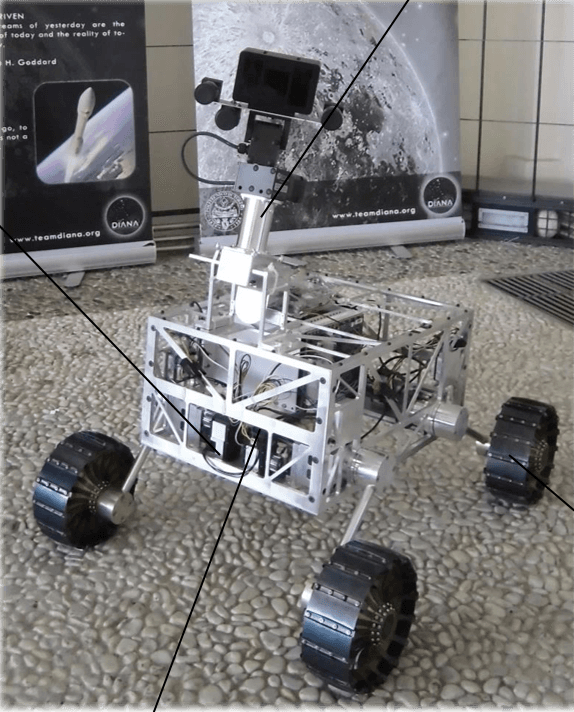
\includegraphics[width=.3\textwidth]{image/amalia.png}
&
		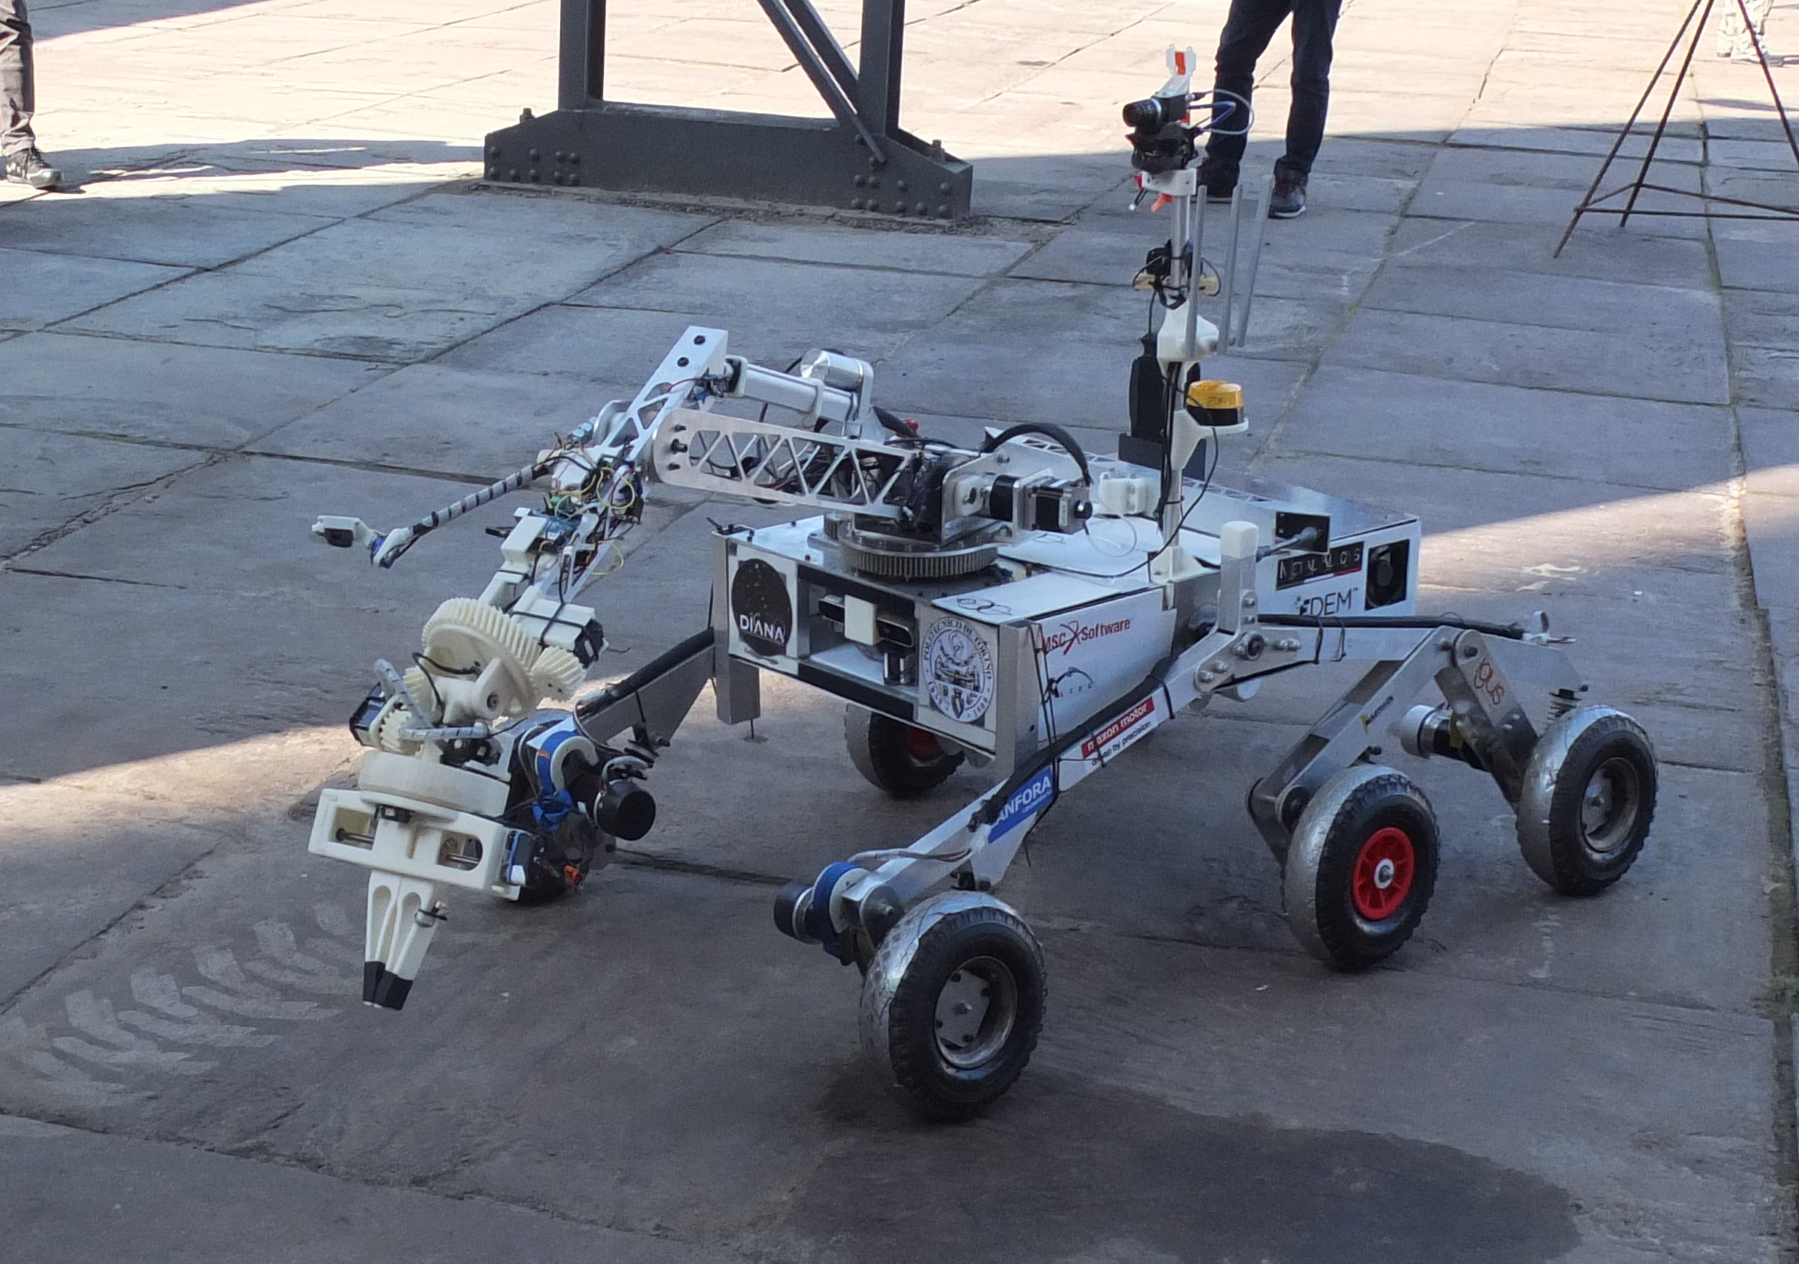
\includegraphics[width=.5\textwidth]{image/toro.jpg}
	\end{tabular}
		\caption{Rover AMALIA E T0-R0}
		\label{fig:amaliatoro}
	
\end{figure}

Il team DIANA ha esperienza decennale nella progettazione e nello sviluppo di modelli di rover per l'esplorazione e l'assistenza e dispone di un set completo di abilità ingegneristiche, ottima conoscenza software ed eccezionali capacità organizzative, gestionali e di lavoro di squadra, cruciali nella produzione di un progetto complesso.\\
Il team intende porre le basi per un nuovo approccio all'ingegneria aerospaziale, contribuendo a portare la robotica spaziale ad un livello più accessibile grazie alla sua tecnica di lavoro innovativa.\\
TRINITY è il prodotto dell'esperienza e della competenza di dieci anni di lavoro e ricerca approfondita, condotta con una chiara visione ed un approccio scientifico.\\
Il team è in crescita dal 2018 e la partecipazione all'\textit{European Rover Challenge} ha avuto un ruolo chiave nel suo sviluppo poiché rappresenta un'opportunità senza precedenti per testare le soluzioni del team e capire dove e come migliorare il suo progetto.

\begin{figure}
	\centering
	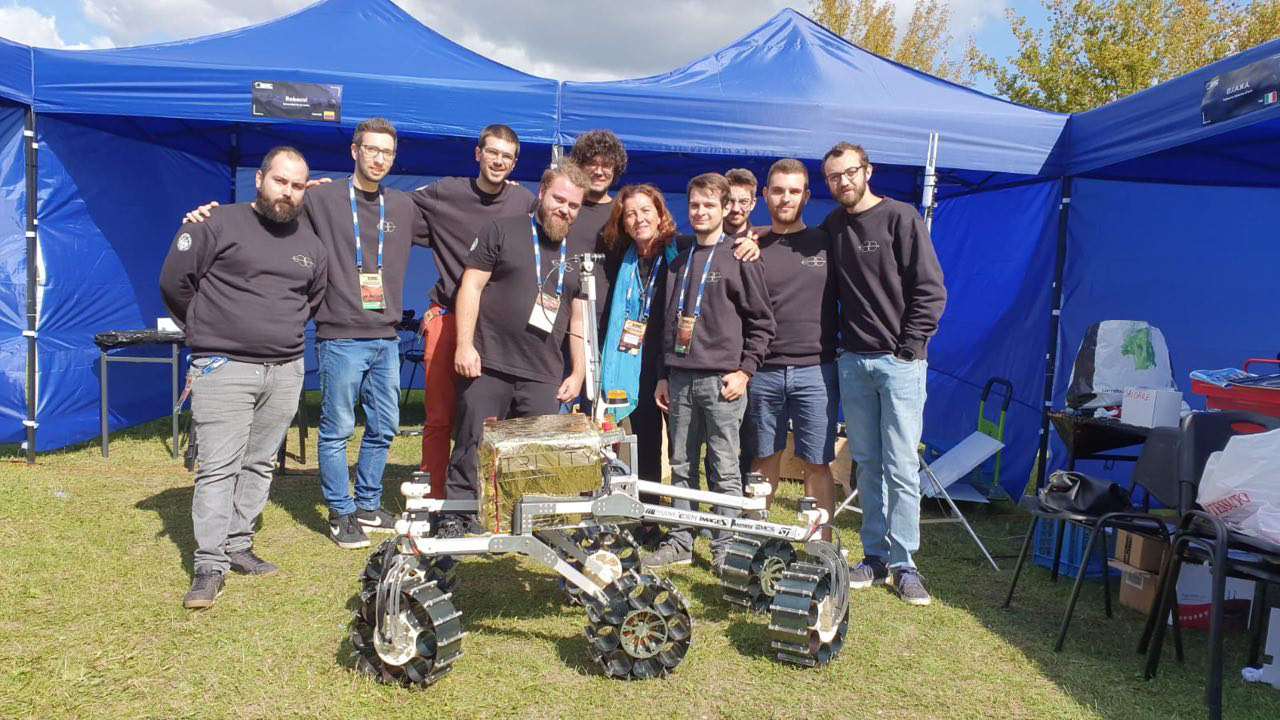
\includegraphics[width=0.6\textwidth]{image/trinityerc.jpeg}
	\caption{Il Team DIANA con TRINITY ad ERC 2019}
	\label{fig:trinityerc}
\end{figure}


Nell'ambito del team DIANA, che sta diventando un forte gruppo di giovani ingegneri che lavorano nella ricerca e nello sviluppo della robotica spaziale, testare il lavoro svolto in laboratorio è un passaggio fondamentale dello sviluppo.\\
Inoltre, il Team DIANA ha vissuto l'European Rover Challenge come un evento eccezionale, in grado di riunire ingegneri appassionati e qualificati in un ambiente internazionale.\\

Pertanto, per essere una fonte di competenza, un occasione di testing e un'opportunità senza precedenti di crescita e raccolta di informazioni sul progetto, la partecipazione all'European Rover Challenge 2019 è senza dubbio un'esperienza necessaria e fondamentale per il Team DIANA.\\

	\section{Dall'esplorazione robotica all'assistenza di equipaggi}
	I Rover di assistenza progettati dal Team DIANA rappresentano dei modelli di future missioni in cui i Rover vengono impiegati nell'assistenza ad un equipaggio umano. \\
	Viene a cadere il presupposto per cui le sonde esplorative operano in scenari \textbf{unmanned} e il ruolo dell'operatore diventa centrale nella progettazione del Robot.\\
	 Esso dovrà avere quanto più possibile un funzionamento autonomo per non sottrarre risorse all'utilizzatore, considerare la presenza di esseri umani nel suo workspace e portare a termine mansioni in ambienti rischiosi per l'essere umano. 
	
	TRINITY è un rover rocker-boogie con ruote elastiche e capacità di sterzo e un braccio robotico e ha un approccio ibrido di operazioni sia autonome che teleoperate.
	
	È un modello ingegneristico di un esploratore marziano e un rover di assistenza in grado di svolgere compiti di navigazione, manutenzione, raccolta e recupero di campioni scientifici.
	
	TRINITY si basa su un design fortemente modulare. Questo tipo di approccio è spesso associato a costi più elevati, elevato consumo di energia e problemi relativi alla comunicazione tra sottosistemi. Tuttavia, da precedenti esperienze il Team ha appreso che un design modulare riduce drasticamente i tempi di sviluppo e produzione e consente di eseguire facilmente modifiche sulla piattaforma esistente per aggiornamenti e correzioni.
	
	
	 
		
	\section{Rover Challenge Series: regolamento e requisiti nelle competizioni tra Rover}
	Le Rover Challenge Series Competitions a cui il Team DIANA prende parte sono competizioni dedicate a studenti dell'area di Ingegneria che mirano a testare i progetti di Rover in uno scenario che simula le mansioni di un Rover di Assistenza.\\
	Si stimola la costituzione di team multidisciplinari che vanno a realizzare un prototipo per competere, corredato da una completa reportistica ispirata alla metodologie attuate nelle principali agenzie spaziali e da documentazione video.\\
	 Viene inoltre richiesta la gestione del team attraverso strumenti di project management e una gestione finanziaria di stampo aziendale.
 
	\begin{figure}
		\centering
		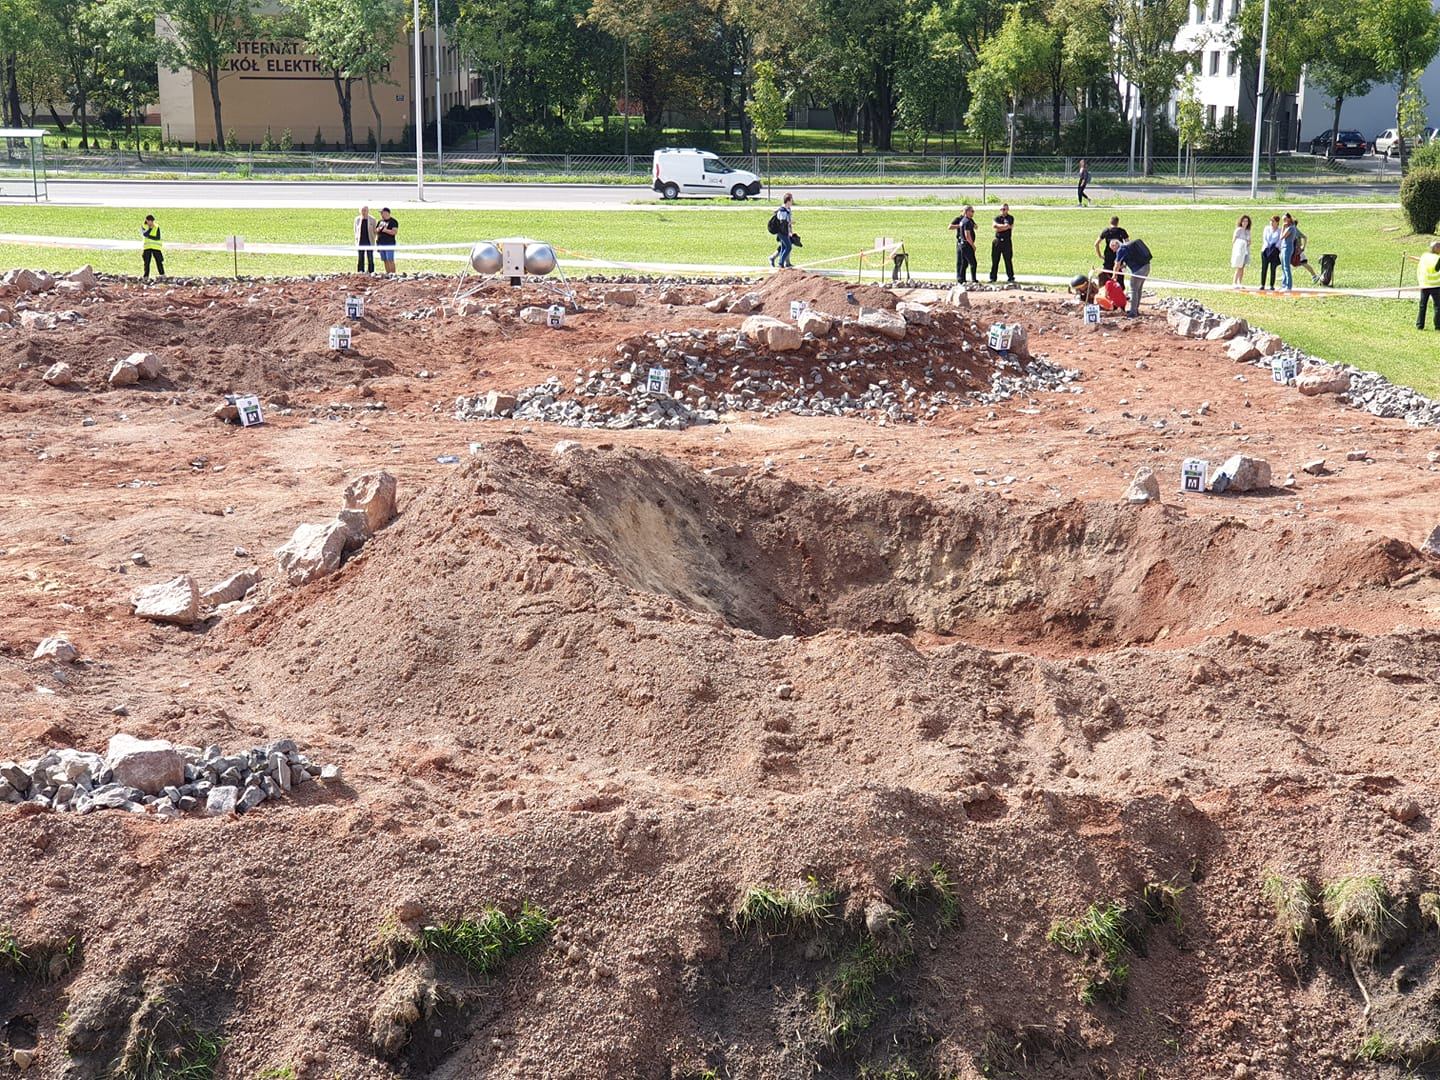
\includegraphics[width=0.6\textwidth]{image/terrain.jpeg}
		\caption{Terreno marziano a European Rover Challenge 2019}
		\label{fig:ercterrain}
	\end{figure}

	\section{Scenari affrontati nelle competizioni e ruolo di un manipolatore robotico}
		Le competizioni si svolgono su un terreno accidentato, realizzato da esperti di terrameccanica, che vanno a simulare il più possibile uno scenario marziano. \\
		Le task vengono svolte in un tempo limitato in cui il Robot è teleoperato, gli operatori sono isolati dalla vista diretta e sono collocati all'interno di una control room. \\
		
		L'unica task che non coinvolge l'uso del manipolatore robotico è quella di \textbf{Navigazione autonoma} che non verrà trattata. 
		Pertanto segue l'analisi degli scenari di utilizzo. 
		\subsection{Manutenzione}
		La  \textbf{Maintanance Task} come definita dal regolamento 
		\textit{ERC 2019 Student Rules} \cite{ERC2019} 
		\newline
		\textit{"The Maintenance Task is intended to demonstrate rovers and teams ability and performance in operating electrical panel on which several switches and other electrical components are mounted. \\
		The Team has to use rover’s manipulating device to set switches to correct positions, measure electrical parameters, set other panel controls and observe device feedback."}

		\newline
		\textbf{Successione di operazioni da svolgere :}
		\begin{enumerate}
		\item Interruttore Principale rotativo, portare in posizione ON;
		\item Switch a levetta gruppo 1 e gruppo 2, posizionare come richiesto dal giudice;
		\item Manopola da ruotare fino al valore richiesto
		\item Misurare la tensione nella presa e riportare il valore al giudice
		\item Inserire la presa trifase industriale
		\item Verifica visiva danneggiamento elementi del pannello 
		\item Riferire al giudice le operazioni svolte in modo autonomo	 
		\end{enumerate}
	
		\begin{figure}
		\centering
		\begin{tabular}{ll}
		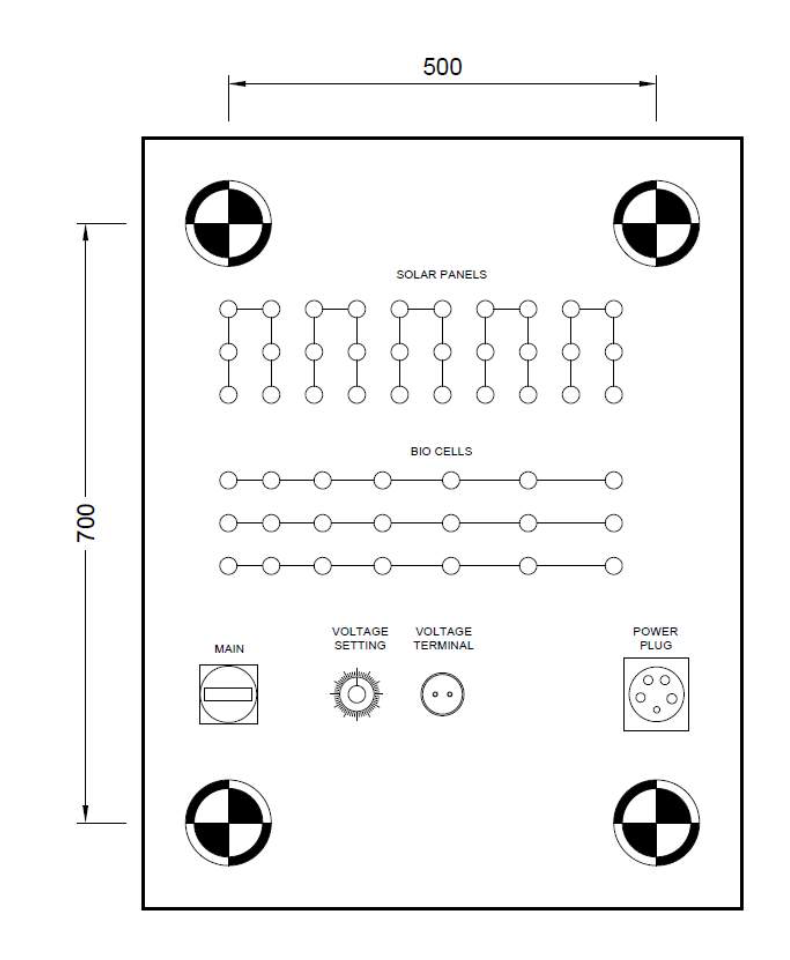
\includegraphics[width=0.4\textwidth]{image/panel.png}
		&
		\includegraphics[width=0.5\textwidth]{image/mainttoro.jpg}
		\end{tabular}
		\caption{Pannello Elettrico e Rover durante la Task}
		\label{fig:maintanance}
		\end{figure}
	
		\subsection{Raccolta di campioni scientifici}
		
		Per qualsiasi missione scientifica o di esplorazione, il rover deve essere in grado di fornire misurazioni di campioni  del suolo e misurarne le proprietà da diversi strati geologici. \\
		In generale, i campioni prelevati da strati più profondi sono più preziosi in ragione delle condizioni atmosferiche sulla superficie dei corpi (gli effetti degli agenti atmosferici spaziali compaiono anche su corpi senza atmosfera dovuti ad esempio alle radiazioni solari).\\
		
		Lo scopo della task è quello di ottenere campioni di strati superficiali e profondi del suolo, prelevati da diverse posizioni specificate dal giudice. \\
		I campioni devono essere conservati nella cache in contenitori appositi.
		\newline
		\textbf{Successione di operazioni da svolgere :} 
		\begin{itemize}
			\item Raggiungere  le aree di campionamento indicate dal giudice 
			\item Raccogliere e collezionare nella cache 4 campioni geologici dal terreno
			\item 3 campioni di superficie da diverse posizioni,
			\item campione profondo (15-30 cm sotto la superficie);
			\item preparare la documentazione fotografica;
			\item Raccogliere diverse misurazioni di campioni o aree di campionamento che potrebbero essere utili
			per la scienza planetaria come ogni peso campione, volume e altri parametri;
			\item Scavare la trincea e documentare il risultato;
			\item Fornire campioni in contenitori sigillati.
		\end{itemize}
		\begin{figure}
			\centering
			\begin{tabular}{ll}
				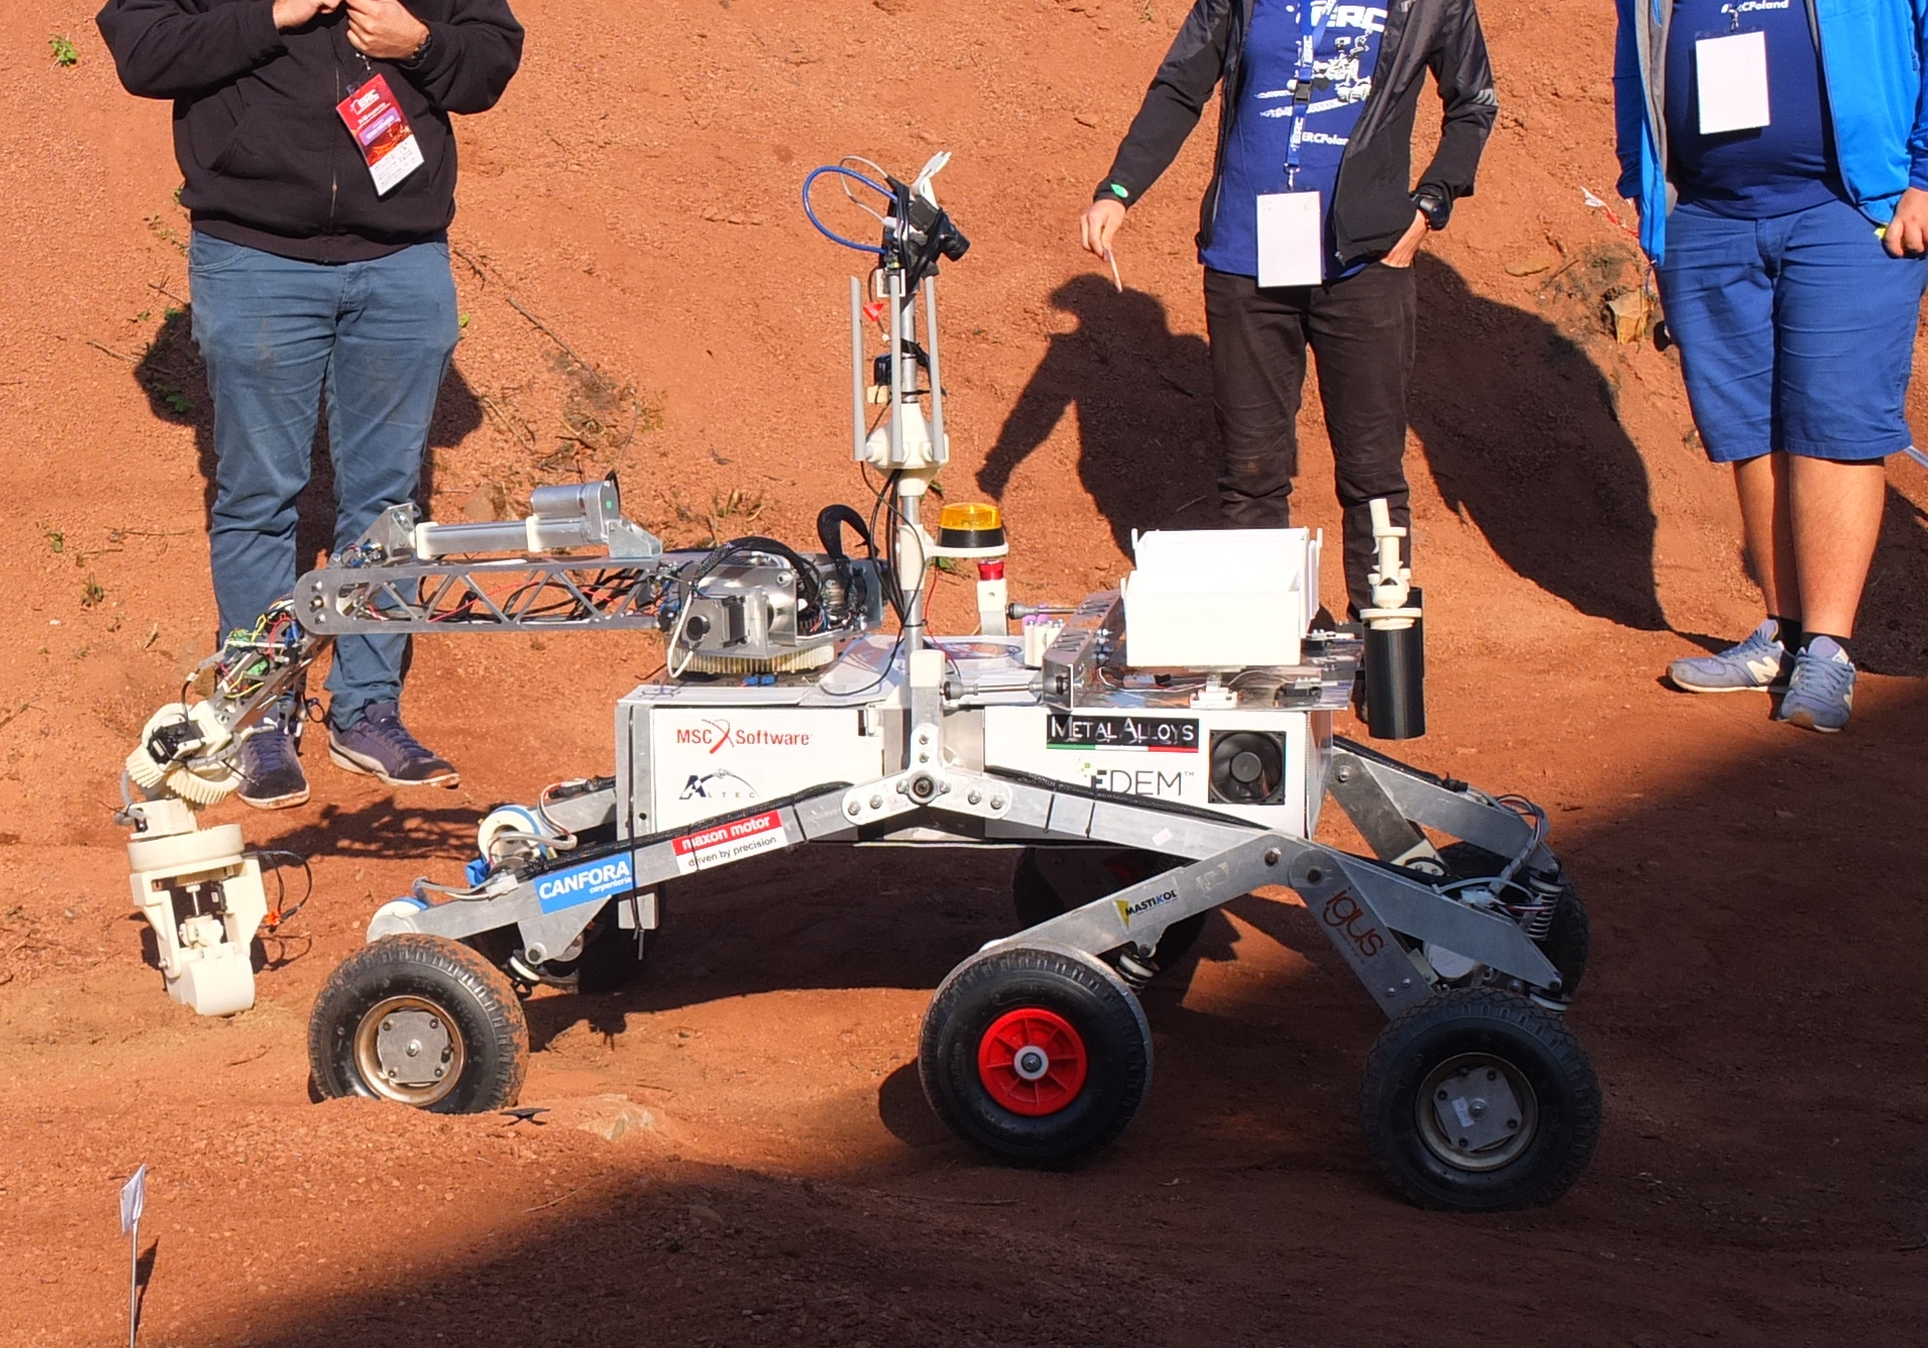
\includegraphics[width=0.5\textwidth]{pictures/sci1.jpg}
				&
				\includegraphics[width=0.5\textwidth]{pictures/sci2.jpg}
			\end{tabular}
			\caption{Rover T0R0 durante la task Scientifica}
			\label{fig:science}
		\end{figure}
		\subsection{Scenario Fetch and Collect}
		La \textbf{Mars Sample Return Mission} dovrebbe essere una missione spaziale finalizzata a raccogliere campioni di roccia e polvere da Marte e riportarli sulla Terra per analisi di laboratorio.
		In questo scenario il rover scientifico lascia a terra campioni sigillati nella cache segnalandone la posizione e per poi continuare il proprio lavoro. \\
		Quindi, un altro rover (caratterizzato da una migliore mobilità e generalmente più veloce) ha la responsabilità di raccoglierli e consegnarli in una posizione specifica. \\
		Quindi il sistema deve essere pronto a cercare ed identificare la cache. Inoltre, il controllo a terra nel ciclo delle operazioni Sample Fetch Return può rallentare la missione, quindi è preferibile automatizzare il più possibile gli elementi della missione.\\
		Alcune missioni specifiche, come il ritorno a terra del campione, impongono requisiti extra sulla progettazione del contenitore che dovrebbe essere utilizzato per la raccolta dei campioni.\\
		Questa attività ha lo scopo di dimostrare la capacità di eseguire la task di recupero della cache. Il team deve raggiungere le posizioni contrassegnate sulla mappa, cercare e raccogliere la cache e posizionarla nel container a bordo con l'orientamento richiesto, quindi consegnare il container con cache alla destinazione finale.\\
		\textbf{Successione di operazioni da svolgere :}
		\begin{itemize}
		\item Raccogli 3 cache da posizioni diverse
		\item Raggiungi l'area in cui è stata rilasciata la cache;
		\item Cerca una cache
		\item Avvicinati alla cache, scatta una foto e raccoglila  
		\item Posizionare la cache nel contenitore a bordo
		\item Consegnare il contenitore con le catture nel luogo designato
		\item Collocare l'intero contenitore con le cache all'interno nel punto contrassegnato
		\end{itemize}
		
		\textbf{Risultati attesi :}
		\begin{itemize}
			\item Dimostrazione di apparecchiature di manipolazione del rover (un braccio robotico o equivalente)
			e le prestazioni dell'operatore nel controllo remoto
			\item Dimostrazione delle capacità di automazione del sistema
			\item Posizionamento delle cache in una posizione corretta nel contenitore
			\item Consegna del container alla destinazione finale
		\end{itemize}
		\begin{figure}
			\centering
			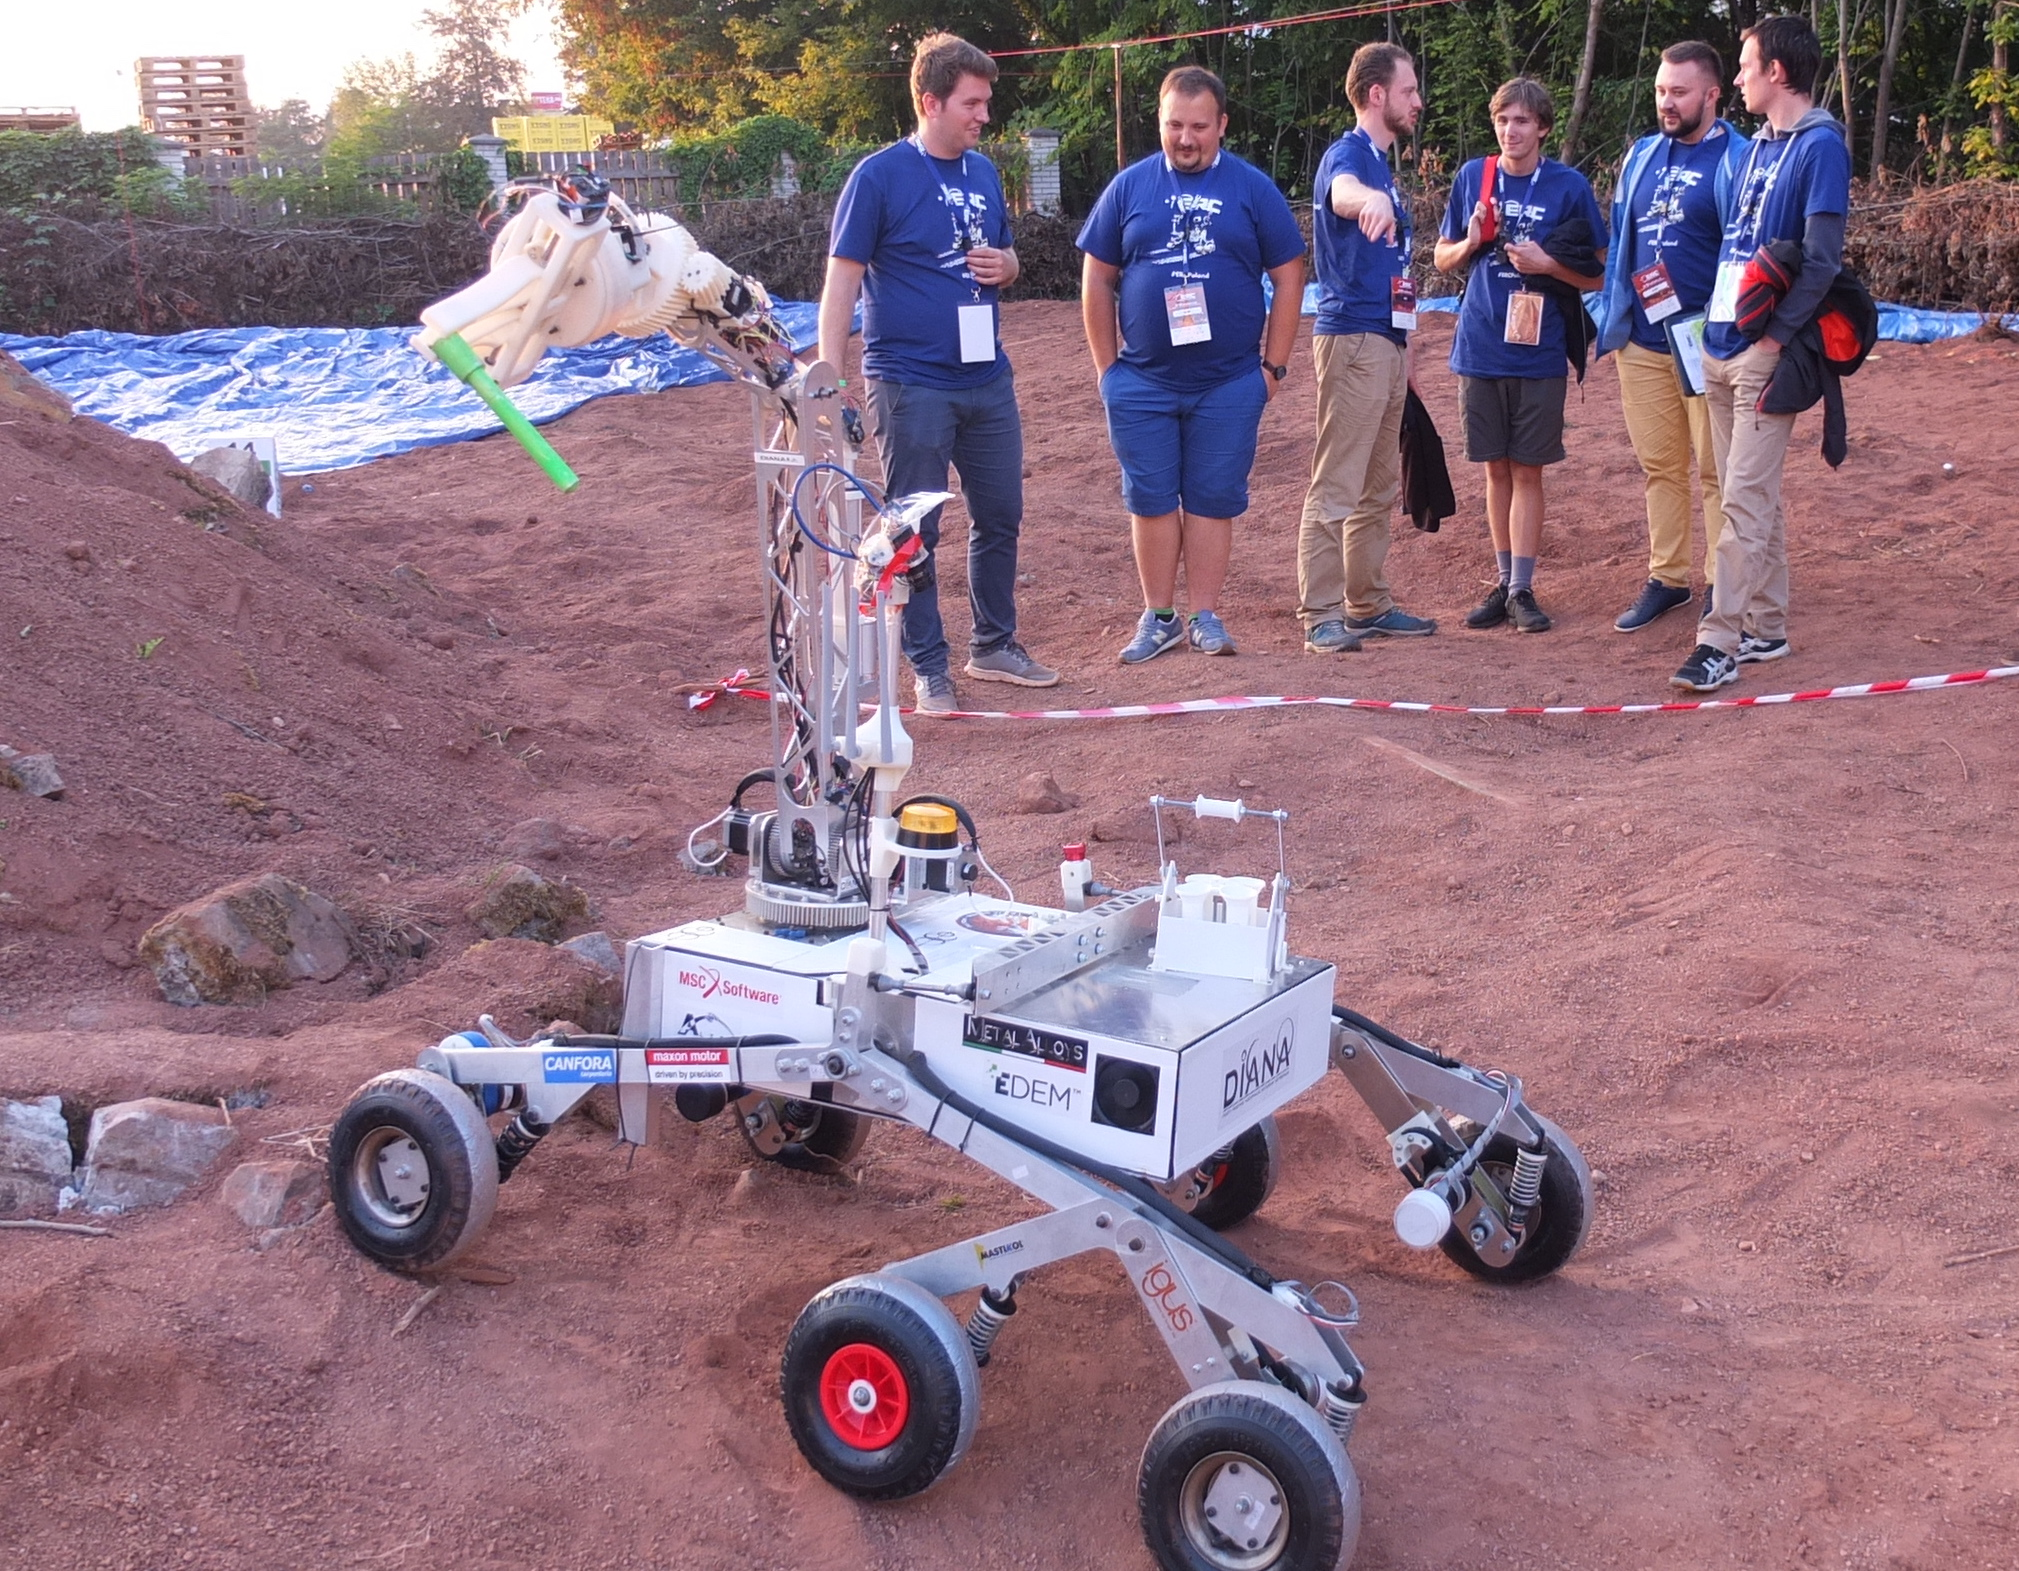
\includegraphics[width=0.5\textwidth]{pictures/cache1.jpg}
			\caption{Il rover T0R0 raccoglie una cache sotto esame della giuria}
			\label{fig:torocache}
		\end{figure}
		\begin{figure}
			\centering
			\begin{tabular}{ll}
				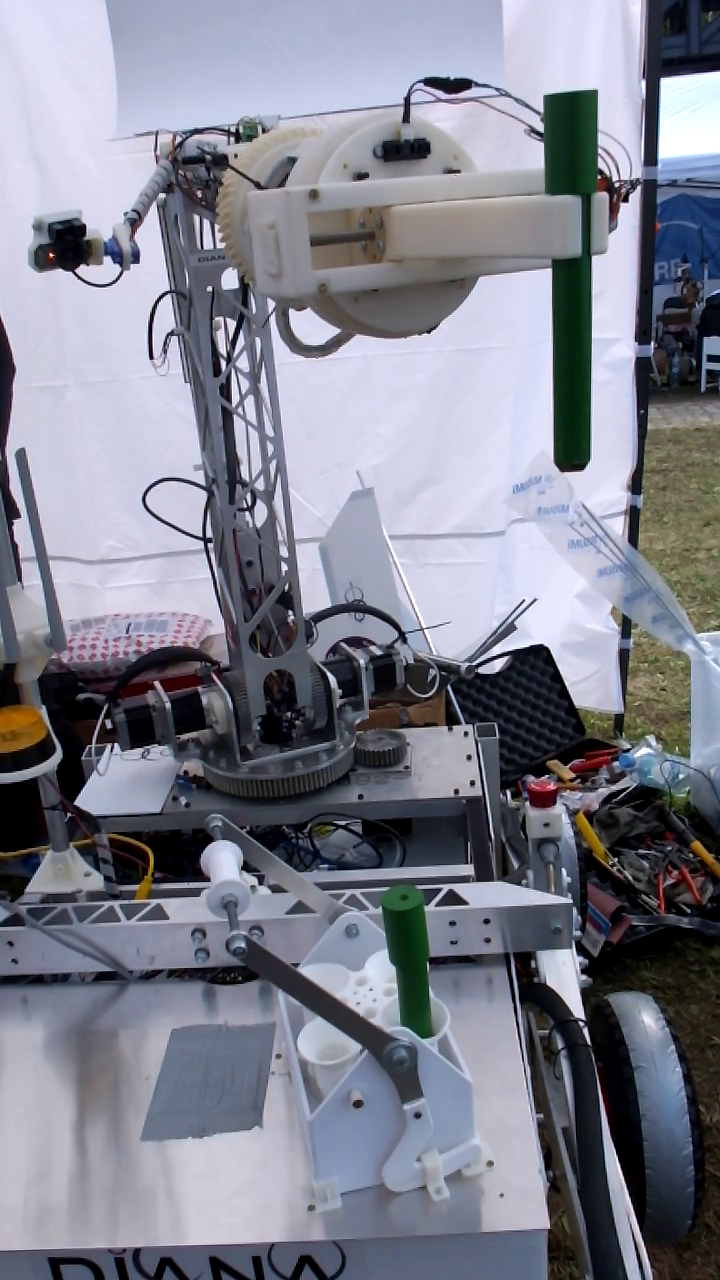
\includegraphics[width=0.4\textwidth]{pictures/cache2.png}
				&
				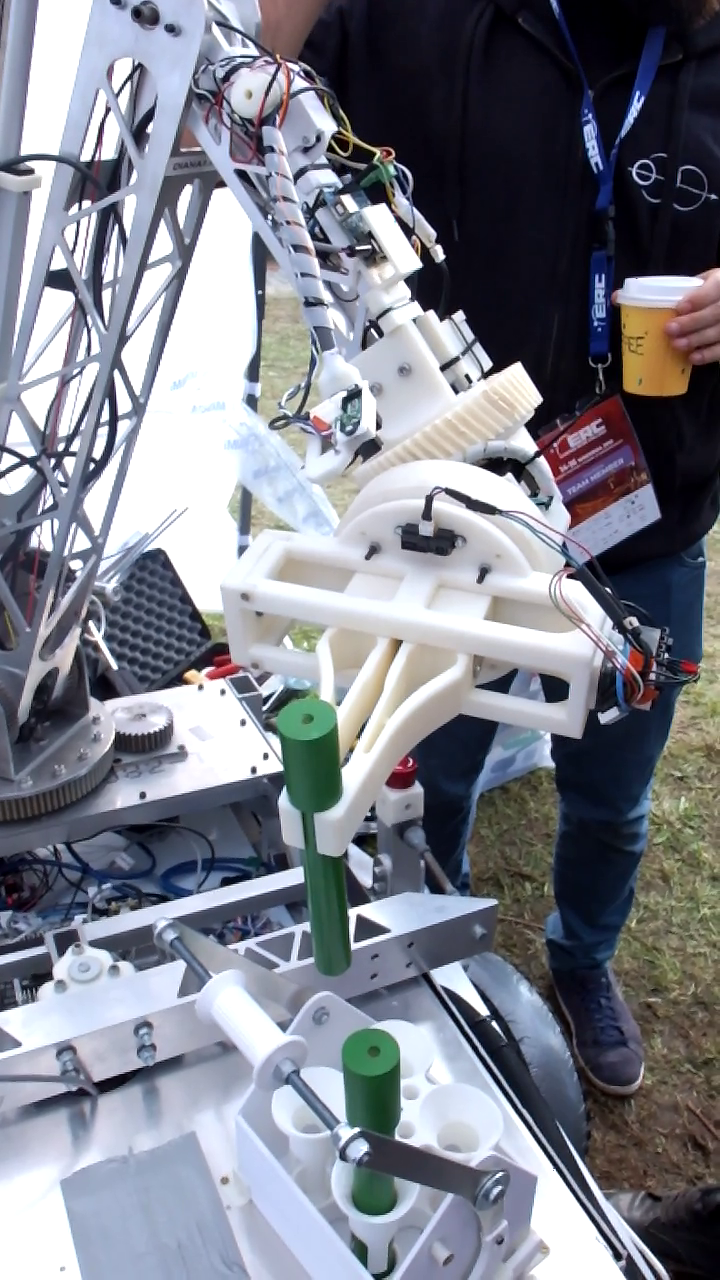
\includegraphics[width=0.4\textwidth]{pictures/cache3.png}
			\end{tabular}
			\caption{Manipolazione della cache, si evidenzia l'abilità di orientamento nello spazio del polso sferico}
			\label{fig:cache}
		\end{figure}
		
	
\chapter{Design di un manipolatore a 6 gradi di libertà}

\section{Analisi preliminare dei requisiti}
Ogni progetto con applicazione aerospaziale, come quello svolto per il \textbf{Rover TRINITY}, parte dall'analisi dei requisiti di progetto e dalla formalizzazione dei requisiti in maniera codificata. \\
La tracciabilità dei requisiti, analizzati a partire da uno scenario di missione e dalla vigente normativa è fondamentale all'interno di un progetto aerospaziale poichè consente di semplificare eventuali sviluppi futuri.\\
La costituzione di un database di requisiti, lezioni apprese ed errori commessi consente di abbattere i costi e le tempisitiche di sviluppo di progetti futuri nel caso in cui i requisiti vengano disattesi evitando la ripetizione di esperimenti ed errori commessi in passato. 

	\renewcommand{\arraystretch}{1.2}
	\begin{longtable}{|p{0.10\textwidth}|p{0.27\textwidth}|p{0.27\textwidth}|p{0.27\textwidth}| } 
		\hline
		 \textbf{ORIG.}& \textbf{REQUISITO}& \textbf{SOLUZIONE     TECNICA}&  \textbf{VALIDAZIONE}\\*  &   &  &      \\* \hline
		\hline
	%ARM ASSUMPTION
		
	ERC &
	Il sottosistema braccio deve essere in grado di raggiungere il terreno, 
	raggiungere tutta la superficie dello chassis del rover, 
	raggiungere 1.5 metri di altezza, 
	manipolare elementi nello spazio tridimensionale &
	Manipolatore robotico antromorfo a 6 assi: dalla letteratura
	è la soluzione con la maggior destrezza	 & Modellazione CAD assieme allo chassis del Rover, Script di calcolo del workspace, modello multibody	\\*	&   &  &      \\* \hline
	
	
	ERC & 
	Il Sottosistema braccio deve essere in grado di sollevare almeno un payload di 5kg &
	Robot attuato da motoriduttori passo-passo, attuatori lineari e servomotori ad elevata coppia
	Trasmissione mediante riduttore a ruote dentate &
	CAD design del braccio, Matlab script del workspace, modello multibody, modello FEM, teoria di Lewis	\\*	&   &  &      \\* \hline
	
	MISSION & Il braccio deve avere elevata velocità operativa senza sacrificare l'accuratezza (target of tool center point of 1$cm^2$) & 
	Controllo in microstep dei motori passo passo, encoder relativo per attuatore lineare
	controllo in posizione dei servomotori &  
	Modello Simulink e cinematica inversa	\\*	&   &  &      \\* \hline

	MISSION & Il braccio deve essere in grado di raggiungere il pannello manutenzione posizionato a 0.5m di distanza 
	con il tool center point perpendicolare & 
	
	Polso Sferico & CAD design, Matlab script, multibody model \\*	&   &  &      \\* \hline
	
\caption{Tabella dei requisiti derivati dal progetto e dal regolamento}	
\end{longtable}
	\section{Obbiettivi del progetto}
	Il progetto finale presentato in questo documento ha come obiettivo quello di raccogliere l'esperienza progettuale fatta nel corso di due anni accademici, nella fattispecie 2018/2019 e 2019/2020, all'interno del Team DIANA. Lo stato del progetto del manipolatore robotico al mio ingresso nel gruppo di progettazione era agli inizi, con delle criticità da affrontare. Nella fattispecie:
	\begin{itemize}
		\item Il workspace doveva essere ancora definito
		\item Il dimensionamento delle trasmissioni e degli attuatori doveva essere validato tramite un modello di calcolo
		\item Il modello di polso ipotizzato era cartesiano e non ancora dotato di attuatori adatti
		\item Il giunto del gomito presentava delle criticità strutturali 
		\item Le fasi di produzione, validazione della controllistica e testing dovevano ancora essere delineate
	\end{itemize}
	
	Pertanto il progetto finale ripercorrà questi punti di cui mi sono occupato avendone la responsabilità della progettazione, lavorando in collaborazione con il gruppo analisi FEM che si è occupato della validazione delle strutture e della loro ottimizzazione.  L'obiettivo di questo percorso di progettazione è illustrare e raccogliere il lavoro svolto all'interno del gruppo di progettazione del manipolatore robotico di cui sono stato responsabile. 
	
	
	\section{Gradi di libertà necessari}
	Il robot antropomorfo debutta in campo industriale all’inizio degli anni Settanta con l’obiettivo di sostituire l’uomo in alcuni passaggi della catena di montaggio che prevedono lo svolgimento di attività usuranti e pericolose. \\
	La struttura meccanica dei robot è costituita da una sequenza di elementi meccanici connessi tra loro da giunti che ne consentono il moto relativo.\\
	 
	 
	 I robot industriali, a cui si ispira il progetto, hanno fondamentalmente lo scopo di manipolare degli oggetti, cioè di muoverli nello spazio controllandone posizione ed orientamento.\\
	  Gli oggetti che i robot si trovano a dover manipolare sono, nella quasi totalità dei casi, riconducibili a corpi solidi. \\
	  Si tratterà quindi di studiarne i possibili movimenti nello spazio per poi definire quelle caratteristiche che la struttura deve possedere per poterli realizzare. \\
	  Infatti l'oggetto, una volta afferrato, è solidale con l'estremità della struttura e quindi ne riproduce fedelmente gli spostamenti. \\
	 Un corpo rigido ha, nello spazio, sei gradi di libertà corrispondenti a tre traslazioni lungo gli assi e tre rotazioni attorno ad essi. 
	 Ciò significa che la sua posizione ed il suo orientamento rispetto ad un sistema di riferimento sono descritte da sei parametri. \\
	 Per rendere piu' intuitiva questa affermazione si immagini di rendere solidale con l'oggetto rigido la terna cartesiana xyz in figura \ref{fig:6DOF}. \\
	 I sei parametri prima citati risultano ora di facile interpretazione: tre definiscono la posizione dell'origine della terna xyz mentre le rimanenti ne individuano l'orientazione. Gli spostamenti corrispondenti sono tre traslazioni (parallelamente agli assi coordinati) e tre rotazioni (attorno agli stessi assi).\\
	  Questo permette di affermare che la struttura di un robot, per poter muovere ed orientare arbitrariamente un corpo nello spazio, ha bisogno di un minimo di sei gradi di libertà. \\
	  Con analoghe considerazioni è facile arrivare a concludere che un corpo rigido, se vincolato a muoversi in un piano, ha tre gradi di libertà. 
	  
	 \begin{figure} [H]
	 	\centering
	 	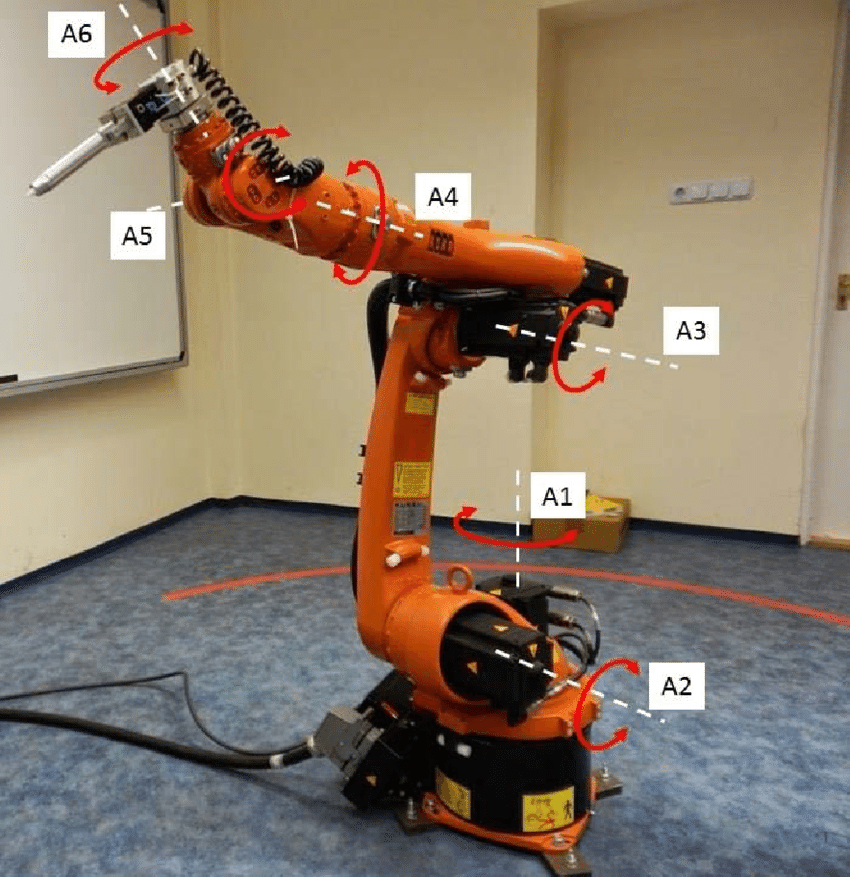
\includegraphics[width=0.6\textwidth]{pictures/KUKA.png}
	 	\caption{Un robot industriale antropomorfo a 6 assi}
	 	\label{fig:KUKA}
	 \end{figure}
	 
	 I robot come quello in figura \ref{fig:KUKA}, sono detti antropomorfi in quanto riproducono abbastanza fedelmente le possibilità di movimento di un braccio umano ed hanno una struttura ben definita con 3 giunti rotoidali per il braccio con il secondo e terzo paralleli tra loro e ortogonali al primo a cui si aggiunge tradizionalmente un polso a 3 gdl rotoidali per ottenere un robot a 6 assi.\\ 
	 
	 L'estremità della struttura di un robot possiede in genere sei diverse possibilità di movimento: tre di traslazione per spostamenti nello spazio e tre di rotazione per l'orientazione.\\
	 Questa divisione dei gradi di libertà in due gruppi con finalità distinte si riflette nella struttura con una specializzazione dei giunti. \\
	 I gradi di libertà principali si occupano di posizionare nello spazio gli oggetti manipolati dal robot, quelli secondari di orientarli. Sono detti principali gli assi che formano il braccio del robot mentre sono detti secondari quelli che costituiscono il polso. Braccio e polso, avendo funzioni diverse, presentano caratteristiche diverse. \\
	 In primo luogo nella realizzazione del braccio si può scegliere se utilizzare giunti rotoidali o prismatici mentre la realizzazione del polso può avvenire solo con giunti rotoidali. \\
	 Inoltre gli elementi strutturali che compongono il braccio hanno una certa lunghezza mentre quelli del polso sono privi di dimensione se si tratta di giunti monocentrici, cioè gli assi di rotazione dei tre giunti idealmente si incontrano in un punto. \\
	 \begin{figure} [H]
	 	\centering
	 	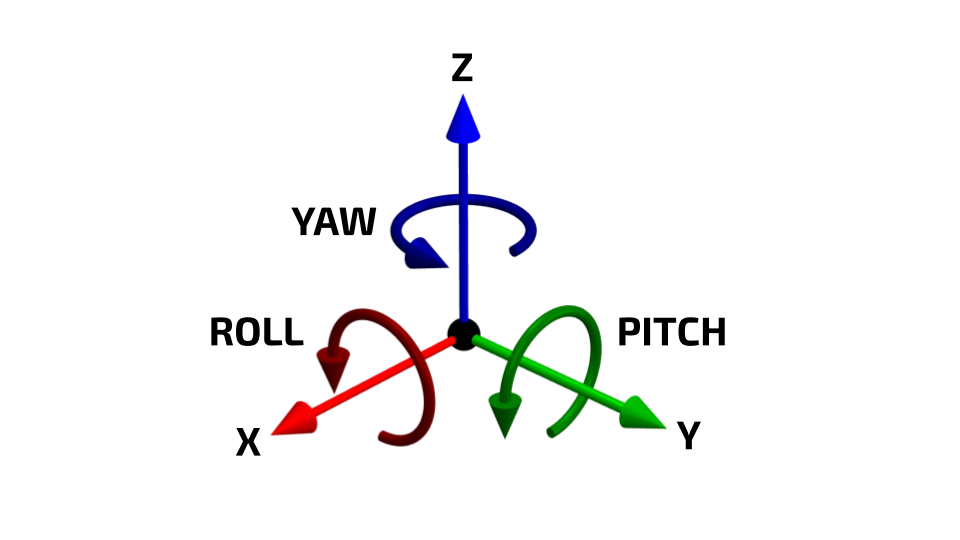
\includegraphics[width=\textwidth]{pictures/6DOF.png}
	 	\caption{6 gradi di libertà di un corpo rigido nello spazio}
	 	\label{fig:6DOF}
	 \end{figure}

\section{Workspace necessario}



\begin{figure} [H]
	\centering
	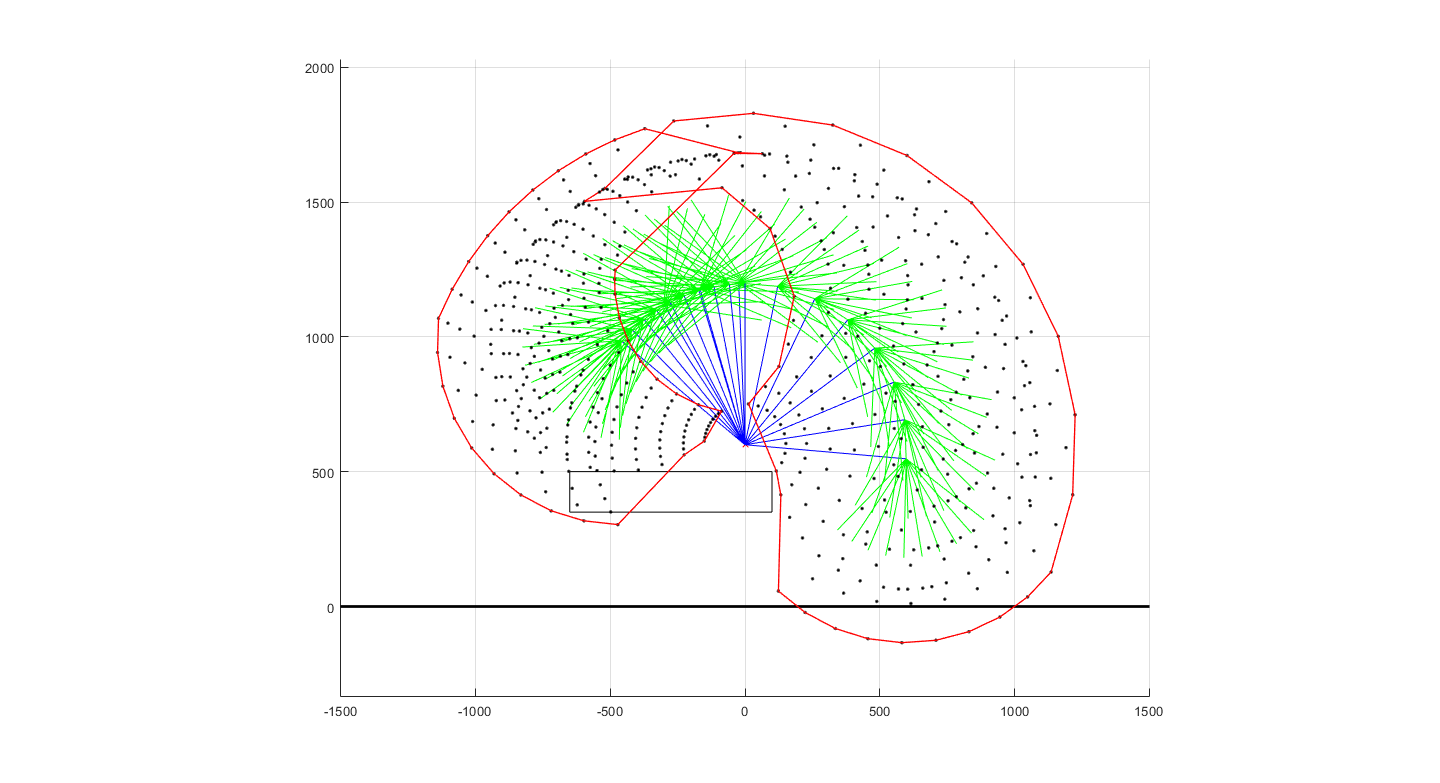
\includegraphics[width=1\textwidth]{Plots/workspace.png}
	\caption{Workspace in vista laterale, è rappresentato il piano dello chassis e i punti raggiunti dal TCP}
	\label{fig:workspace}
\end{figure}

Il volume di lavoro può essere considerato, in prima approssimazione, come una porzione di sfera.
Il workspace richiesto per il manipolatore deriva dalle richieste del regolamento e dallo scenario operativo e si può riassumere nella necessità di raggiungere un altezza che va da 1,5 metri e quella del suolo e di operare sullo chassis del rover per depositare oggetti e campioni. \\
Il workspace è stato valutato attraverso un calcolo iterativo di cinematica diretta in cui la struttura è statz parametrizzata attraverso le lunghezze dei link. L'obiettivo è quello di realizzare uno spazio di lavoro sufficiente rappresentando graficamente la posizione del \textbf{Tool Center Point} per ogni iterazione in una vista laterale in figura \ref{fig:workspace}. \\
\begin{lstlisting}[language=Matlab]
%%% Dati Rover per il calcolo del workspace%%%

% CHASSIS
 
h1=500; %altezza lato superiore chassis [mm]
h2=100; %distanza tra giunto spalla e chassis [mm]
h0=h1+h2; %distanza giunto spalla da terra [mm]

% ARM
%lunghezze link: braccio ,avambraccio , distanza tra polso e TCP   [mm]
l=[600 367 315];

% escursione angoli giunti: 

a=[-5 120   %spalla(zero: link parallelo al terreno che punta verso fronte rover)
                  % 125 gradi di escursione
33 129   	 %elbow (zero: link parallelo al link precedente che punta fronte rover)
 
	              %96 gradi di escursione
-90 90]; 	 %second wrist joint (zerolink parallelo al precedente che punta fronte rover) 
             	  %180 gradi di escursione

%% Calcolo cinematica diretta per braccio rivolto di fronte

j1=[0 h0]; %Posizione giunto spalla
i=0;

for a1=deg2rad(linspace(a(1,1),a(1,2),10)) 

%giunto gomito
for a2=deg2rad(linspace(a(2,1),a(2,2),10))

%giunto polso
for a3=deg2rad(linspace(a(3,1),a(3,2),3))

j2=[j1(1)+l(1)*cos(a1),j1(2)+l(1)*sin(a1)];
j3=[j2(1)+l(2)*cos(a1-a2),j2(2)+l(2)*sin(a1-a2)];
j4=[j3(1)+l(3)*cos(a1-a2-a3),j3(2)+l(3)*sin(a1-a2-a3)]; %TCP

i=i+1; 
plot([j1(1),j2(1)],[j1(2),j2(2)],'b')
plot([j2(1),j3(1)],[j2(2),j3(2)],'g')
% plot([j3(1),j4(1)],[j3(2),j4(2)],'c')
%escluso dalla visualizzazione il polso 
plot(j4(1),j4(2),'.k')
x(i)=j4(1);
y(i)=j4(2);
pause(0.00001)
end         
end
end 

%frontiera
% scatter(x,y)
k = boundary(x(:),y(:));
plot(x(k),y(k),'r','LineWidth',1)
hold on

\end{lstlisting}

Questo listato contiene i valori finali che sono stati scelti per costruire il workspace in figura \ref{fig:workspace}, verificato graficamente tramite la linea di terra e la forma dello chassis riportata nel grafico. Le linee rosse rappresentano la frontiera dello spazio del workspace e sono i punti di estremo raggiungibili dal Tool Center Point. I punti in nero rappresentano invece le coordinate raggiunte ma che non si trovano alla frontiera, si è scelto di iterare il calcolo per intervalli di 10 gradi in modo da non riempire troppo la figura. Le linee verdi e blu invece rappresentano braccio e avambraccio.


Una volta decise delle lunghezze dei link principali è stato possibile costruire i primi modelli cad della struttura del robot al fine di realizzare un modello dinamico e non solo più cinematico. \\
L'abilità di raggiungere facilmente delle posizioni intorno al basamento, il fatto che il robot possa scendere al di sotto della quota della base, estendersi verso l'alto e infine depositare degli oggetti alle sue spalle sono i requisiti principali per il progetto. 
Molte applicazioni pratiche non richiedono necessariamente tutte queste possibilità ma, in generale, si può dire che tutto ciò che gli altri robot possono fare, può essere fatto con più facilità da un robot antropomorfo.\\



\section{Descrizione del modello di Robot}
La configurazione scelta è quella di un manipolatore antropomorfo a 6 assi. \\
La struttura per i giunti principali è realizzata tramite link costituiti da profilati in alluminio estruso e parti lavorate in alluminio mentre le cerniere sono realizzate da alberi in acciaio supportati da cuscinetti a strisciamento a basso coefficiente di attrito. \\
I giunti secondari sono collocati nel \textbf{Polso Sferico} all'estremità, un componente in manifattura additiva che verrà trattato più ampiamente in seguito. \\
Il polso è costituito da un insieme di non più di tre giunti rotoidali realizzati alla scopo di permettere l'orientazione dell'utensile di manipolazione del robot. \\
Sarebbe molto interessante che i tre assi, attorno a cui avvengono le rotazioni, si incontrino in un ben determinato punto del pezzo manipolato, cosi' che l'operazione di orientamento non vada a modificare la sua posizione nello spazio di lavoro. \\
Si pensi, come esempio, ad un robot utilizzato in un'applicazione di avvitatura, il cui polso sia realizzato in modo tale che i tre assi di rotazione si incontrino esattamente nella punta del giraviti.\\
 Ciò significa che la vite può essere orientata, ad esempio per renderla perpendicolare alla superficie del pezzo che ospita il foro filettato, senza che questa vari la sua posizione nello spazio che risulterebbe governata soltanto dai giunti principali. \\
 Poichè è molto difficile realizzare in pratica un polso di questo tipo, quelli dei robot industriali e quello realizzato per manipolatore del Rover TRINITY hanno il punto di incontro degli assi di rotazione contenuto all'interno del polso stesso.

	\begin{figure}
	\centering
	\includegraphics[width=0.7\textwidth]{pictures/ARM.png}
	\caption{Render del modello CAD preliminare del robot}
	\label{fig:render}
\end{figure}
	\begin{figure}
	\centering
	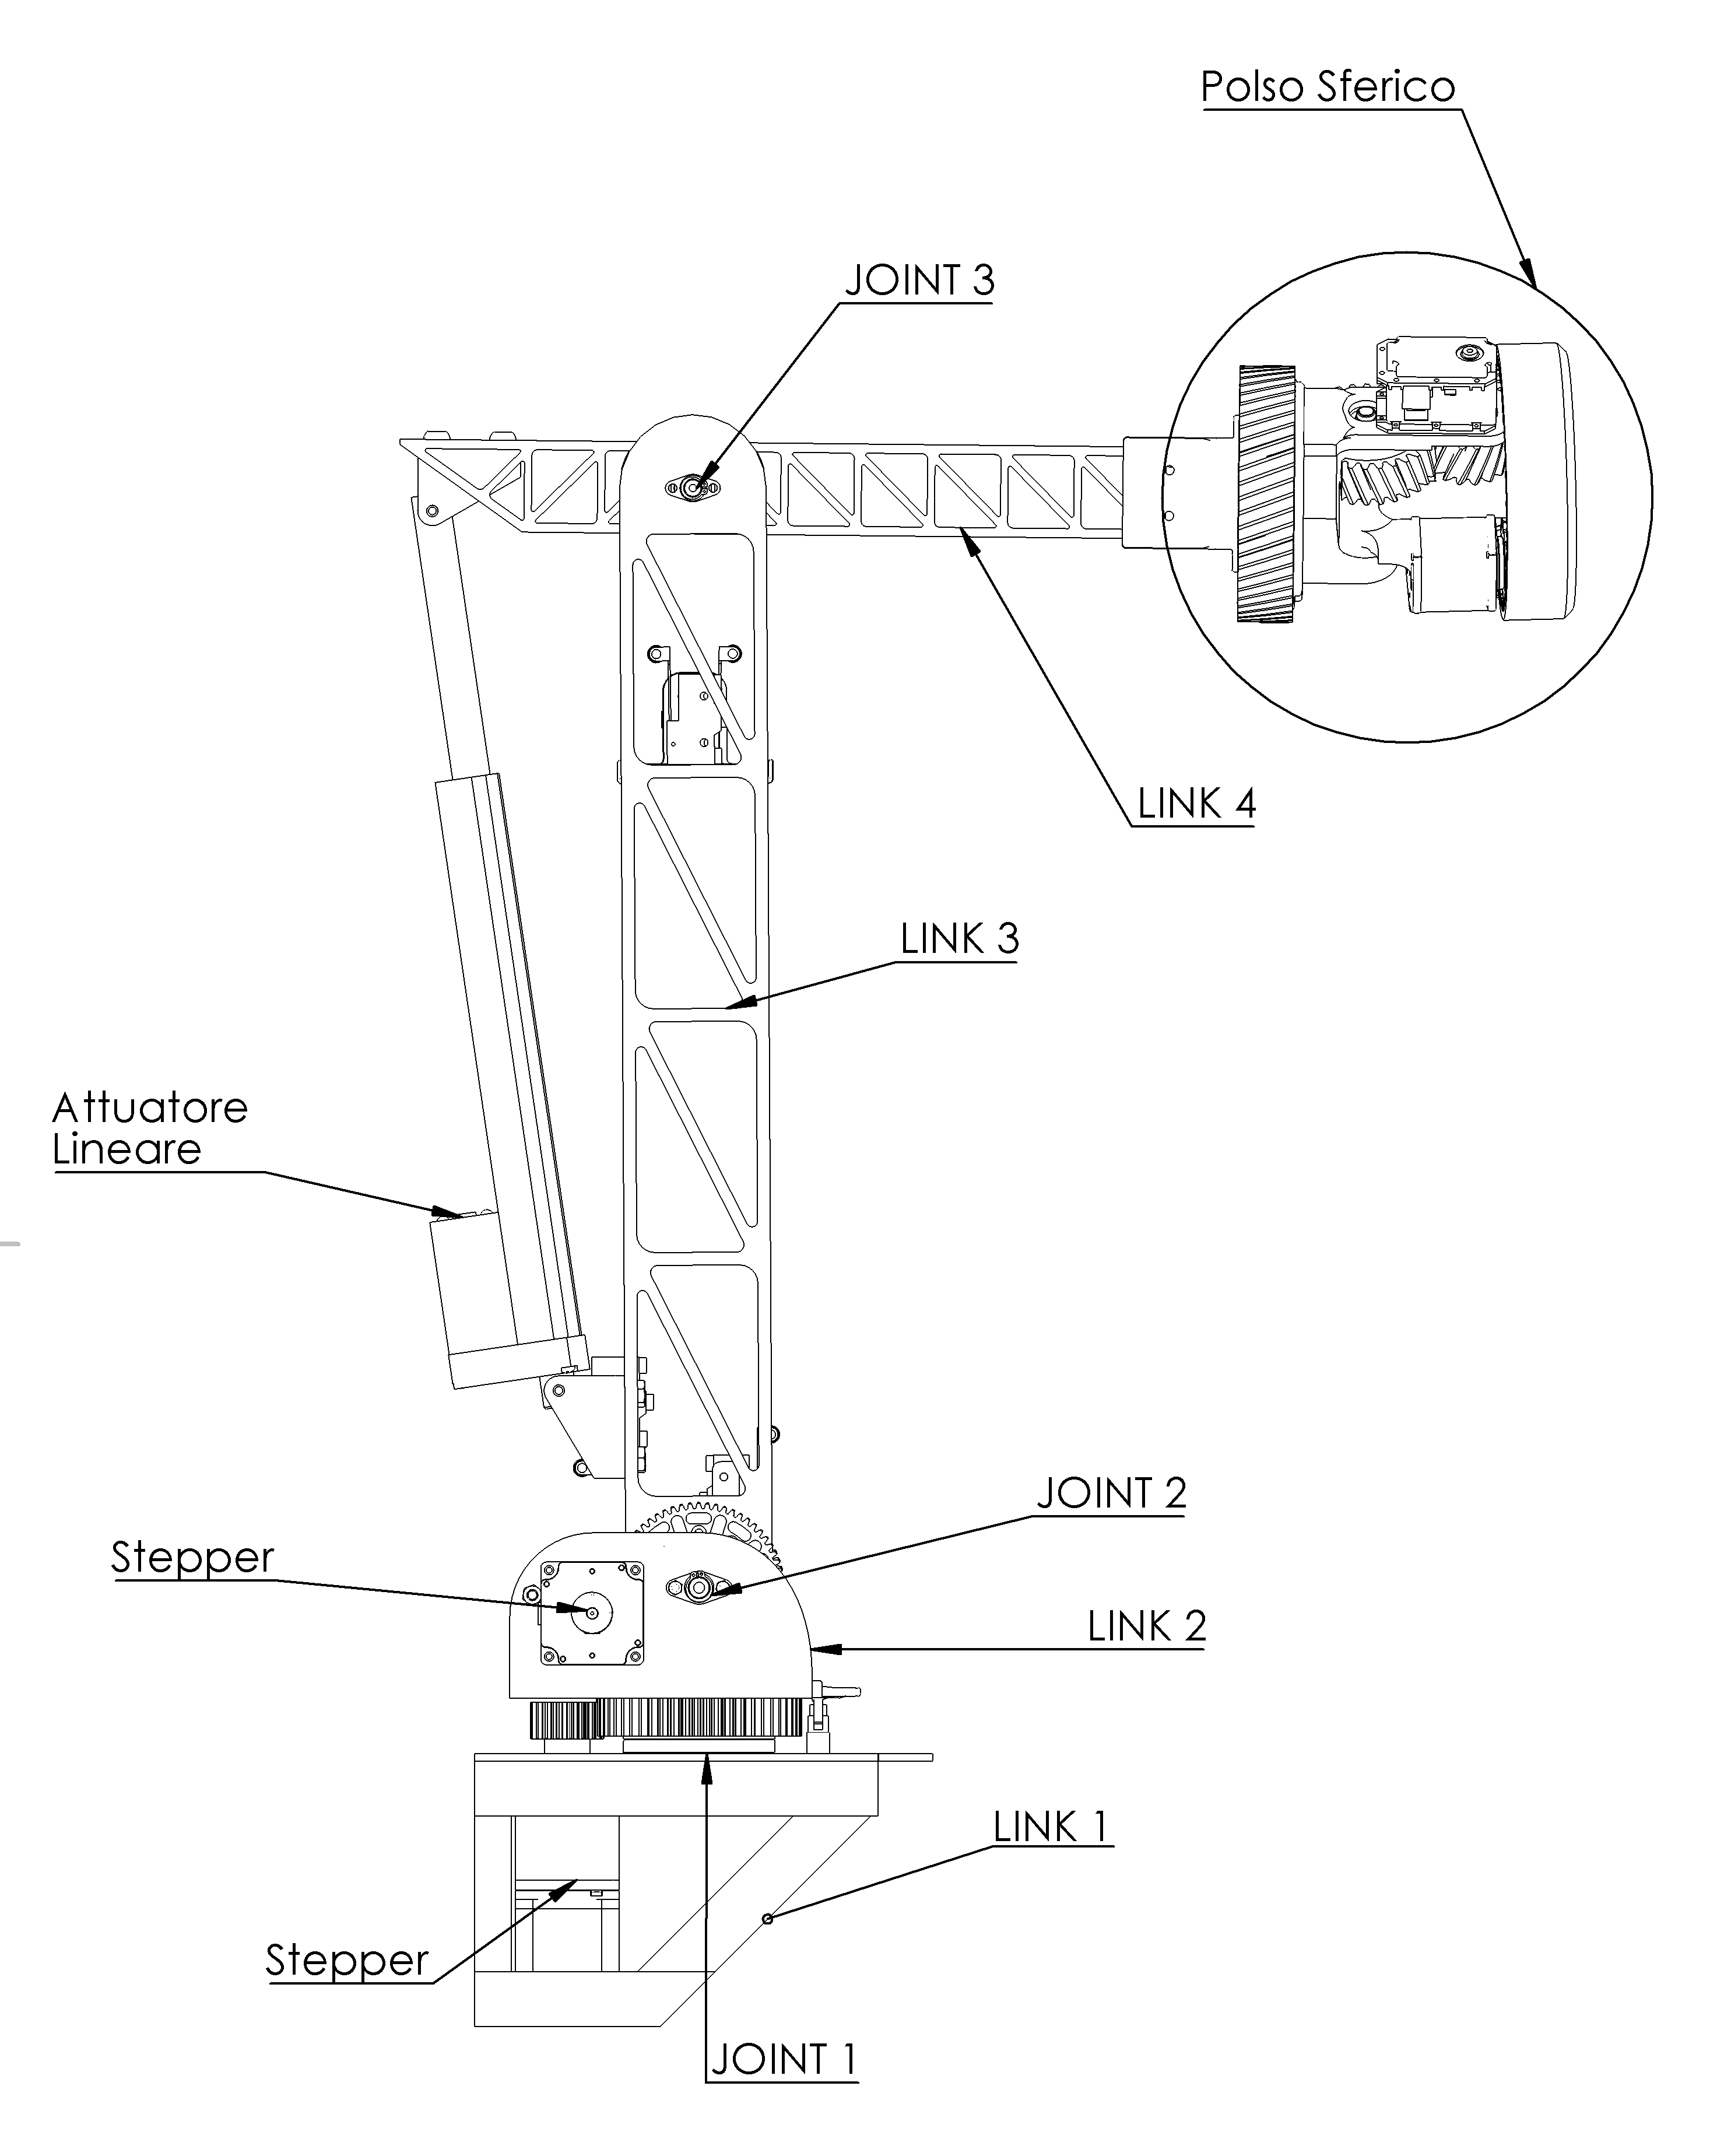
\includegraphics[width=0.7\textwidth]{Screen/ARMBollato.png}
	\caption{Schema delle componenti}
	\label{fig:bollatura}
\end{figure}
Il robot in figura \ref{fig:render} è schematizzato nel disegno \ref{fig:bollatura} e nel capitolo 3 verrà analizzato il dimensionamento degli  \textbf{Attuatori Passo Passo} e dell'\textbf{Attuatore Lineare} mentre al \textbf{Polso Sferico} sarà dedicato il capitolo 4. 

	
	\section{Modello multibody}
	La costruzione di un modello multibody del robot è fondamentale al fine di avere uno strumento di analisi delle prestazioni richieste agli attuatori e poter selezionare dei componenti adatti sul mercato. 
	Per l'analisi della dinamica del robot è stato costruito un modello multibody attraverso il software \textit{MSC Adams}. \\
	Un sistema dinamico multibody consiste in un insieme di corpi solidi connessi tra loro tramite giunti che ne limitano o impongono il relativo movimento. Lo studio della dinamica multibody è l’analisi di come questi sistemi si muovono sotto l’influenza di specifiche forze, detta anche dinamica diretta. Lo studio del problema opposto, cioè di quali forze sono necessarie a far muovere il sistema meccanico in un modo specifico è detta dinamica inversa.\\
	La possibilità di studio della dinamica inversa ha permesso di studiare le prestazioni richieste agli attuatori del robot e dimensionare di conseguenza i componenti meccanici della trasmissione. 
	Una volta eseguita la simulazione è possibile visualizzare le misure richieste e graficare i dati raccolti con lo strumento \textit{Adams/PostProcessor}.  
		\begin{figure}
		\centering
		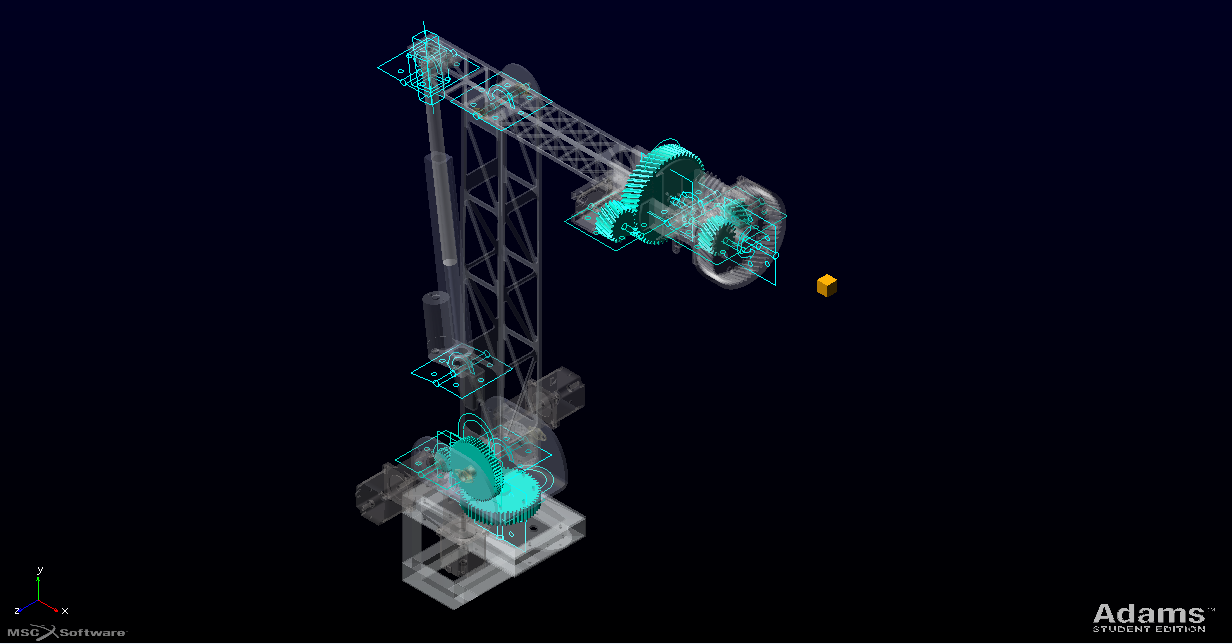
\includegraphics[width=0.7\textwidth]{Screen/Model1.png}
		\caption{Modello del Robot in ambiente Adams, in ciano le icone dei giunti e le trasmissioni mediante ruote dentate}
		\label{fig:adamsmodel}
	\end{figure}
	
	Il modello del robot \ref{fig:adamsmodel} è stato costruito a partire dal modello CAD preliminare \ref{fig:render} modellato in ambiente \textit{SolidWorks} importato nello spazio di lavoro di \textit{Adams/View}.\\
	 I singoli componenti sono stati dotati delle relative matrici di inerzia riferite a un sistema di riferimento favorevole al calcolo dall'output di proprietà di massa del CAD,  riferite ad un analogo \textit{Marker} del modello di simulazione. \\
	 Così facendo la simulazione permetterà di calcolare le forze necessarie affinchè si rispettino le leggi di moto imposte ai giunti.
			\begin{figure}
			\centering
			\begin{tabular} {ll}
		
			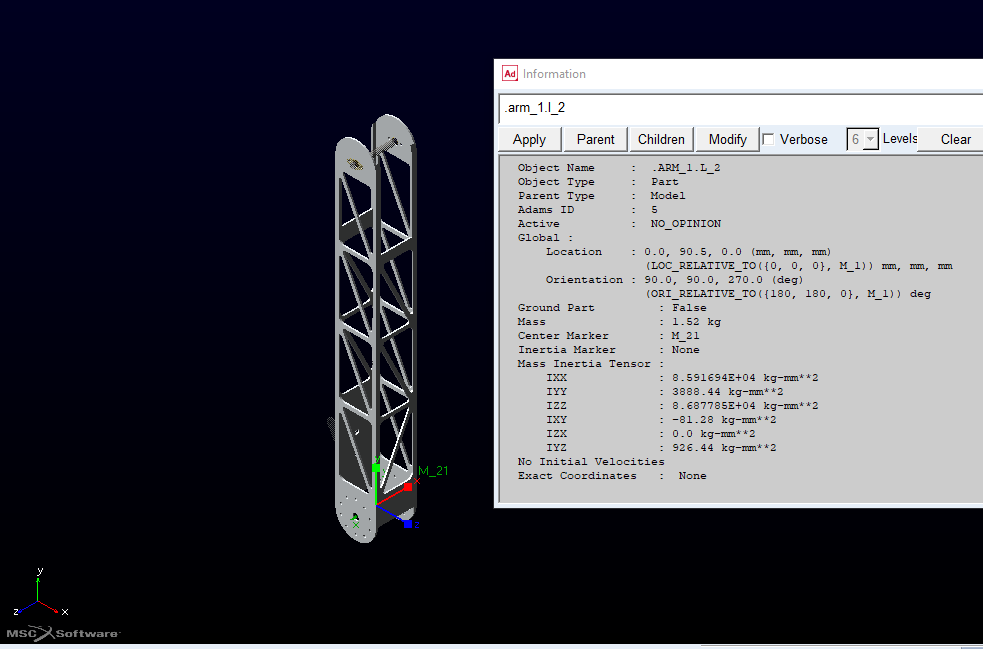
\includegraphics[height=4cm, keepaspectratio]{Screen/inertia.png}
			&
			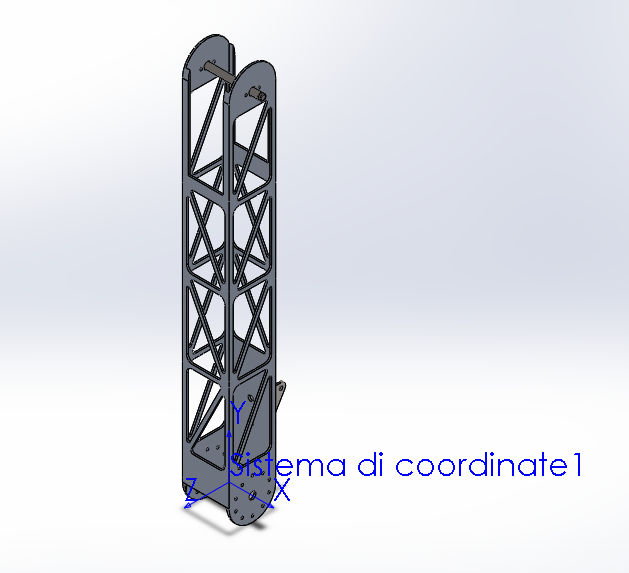
\includegraphics[height=4cm, keepaspectratio]{Screen/coordinate.png}
			\end{tabular}
			\caption{Proprietà inerziali del componente e sistema di coordinate nel CAD}
			\label{fig:inertia}
			\end{figure}
	 Il modulo \textit{Adams/Machinery} consente di modellare le trasmissioni mediante accoppiamento di ruote dentate e di simularne il comportamento con vari livelli di approssimazione. \\
	 Nella fattispecie si è scelto l'approccio semplificato che studia il problema di contatto mediante metodo analitico monodimensionale, in modo da fornire un confronto ed una verifica del dimensionamento realizzato. 	

\chapter{Attuatori per un progetto di robotica low-cost} 
Il progetto dei Rover che partecipano alle Rover Challenge Series competitions è sottoposto ad un vincolo di costo molto importante.\\
 Difatti nella gara progettuale è posto un limite di costo per l'intero progetto che varia da competizione a competizione o dove non ci fosse un limite esplicito, è sicuramente premiata l'economia e l'utilizzo di componenti standard già disponibili sul mercato. \\
Questo vincolo si rivela molto importante nella scelta degli attuatori e relativa elettronica di controllo essendo essi i componenti più costosi in un progetto di questo tipo. \\
Per i giunti di posizionamento sono stati impiegati motoriduttori passo-passo e un attuatore lineare mentre per i giunti del polso sono stati scelti dei servomotori digitali per applicazioni robotiche. 
	\section{Motoriduttori Passo-Passo}
	I motoriduttori passo-passo scelti sono commercializzati dalla Phidgets ed offrono un potente e robusto attuatore a basso costo. \\
	Hanno risoluzione angolare di 0.023° ed una coppia massima di 23 Nm, sono dotati di flangiatura standard NEMA-23 ed albero di uscita di diametro $\phi 12$ con sede linguetta e anello elastico per accoppiare una ruota dentata. 
	Il secondo alberino di uscita permette di ospitare un encoder ottico per realizzare un controllo in posizione ad anello chiuso.\\
		\begin{figure}
		\centering
		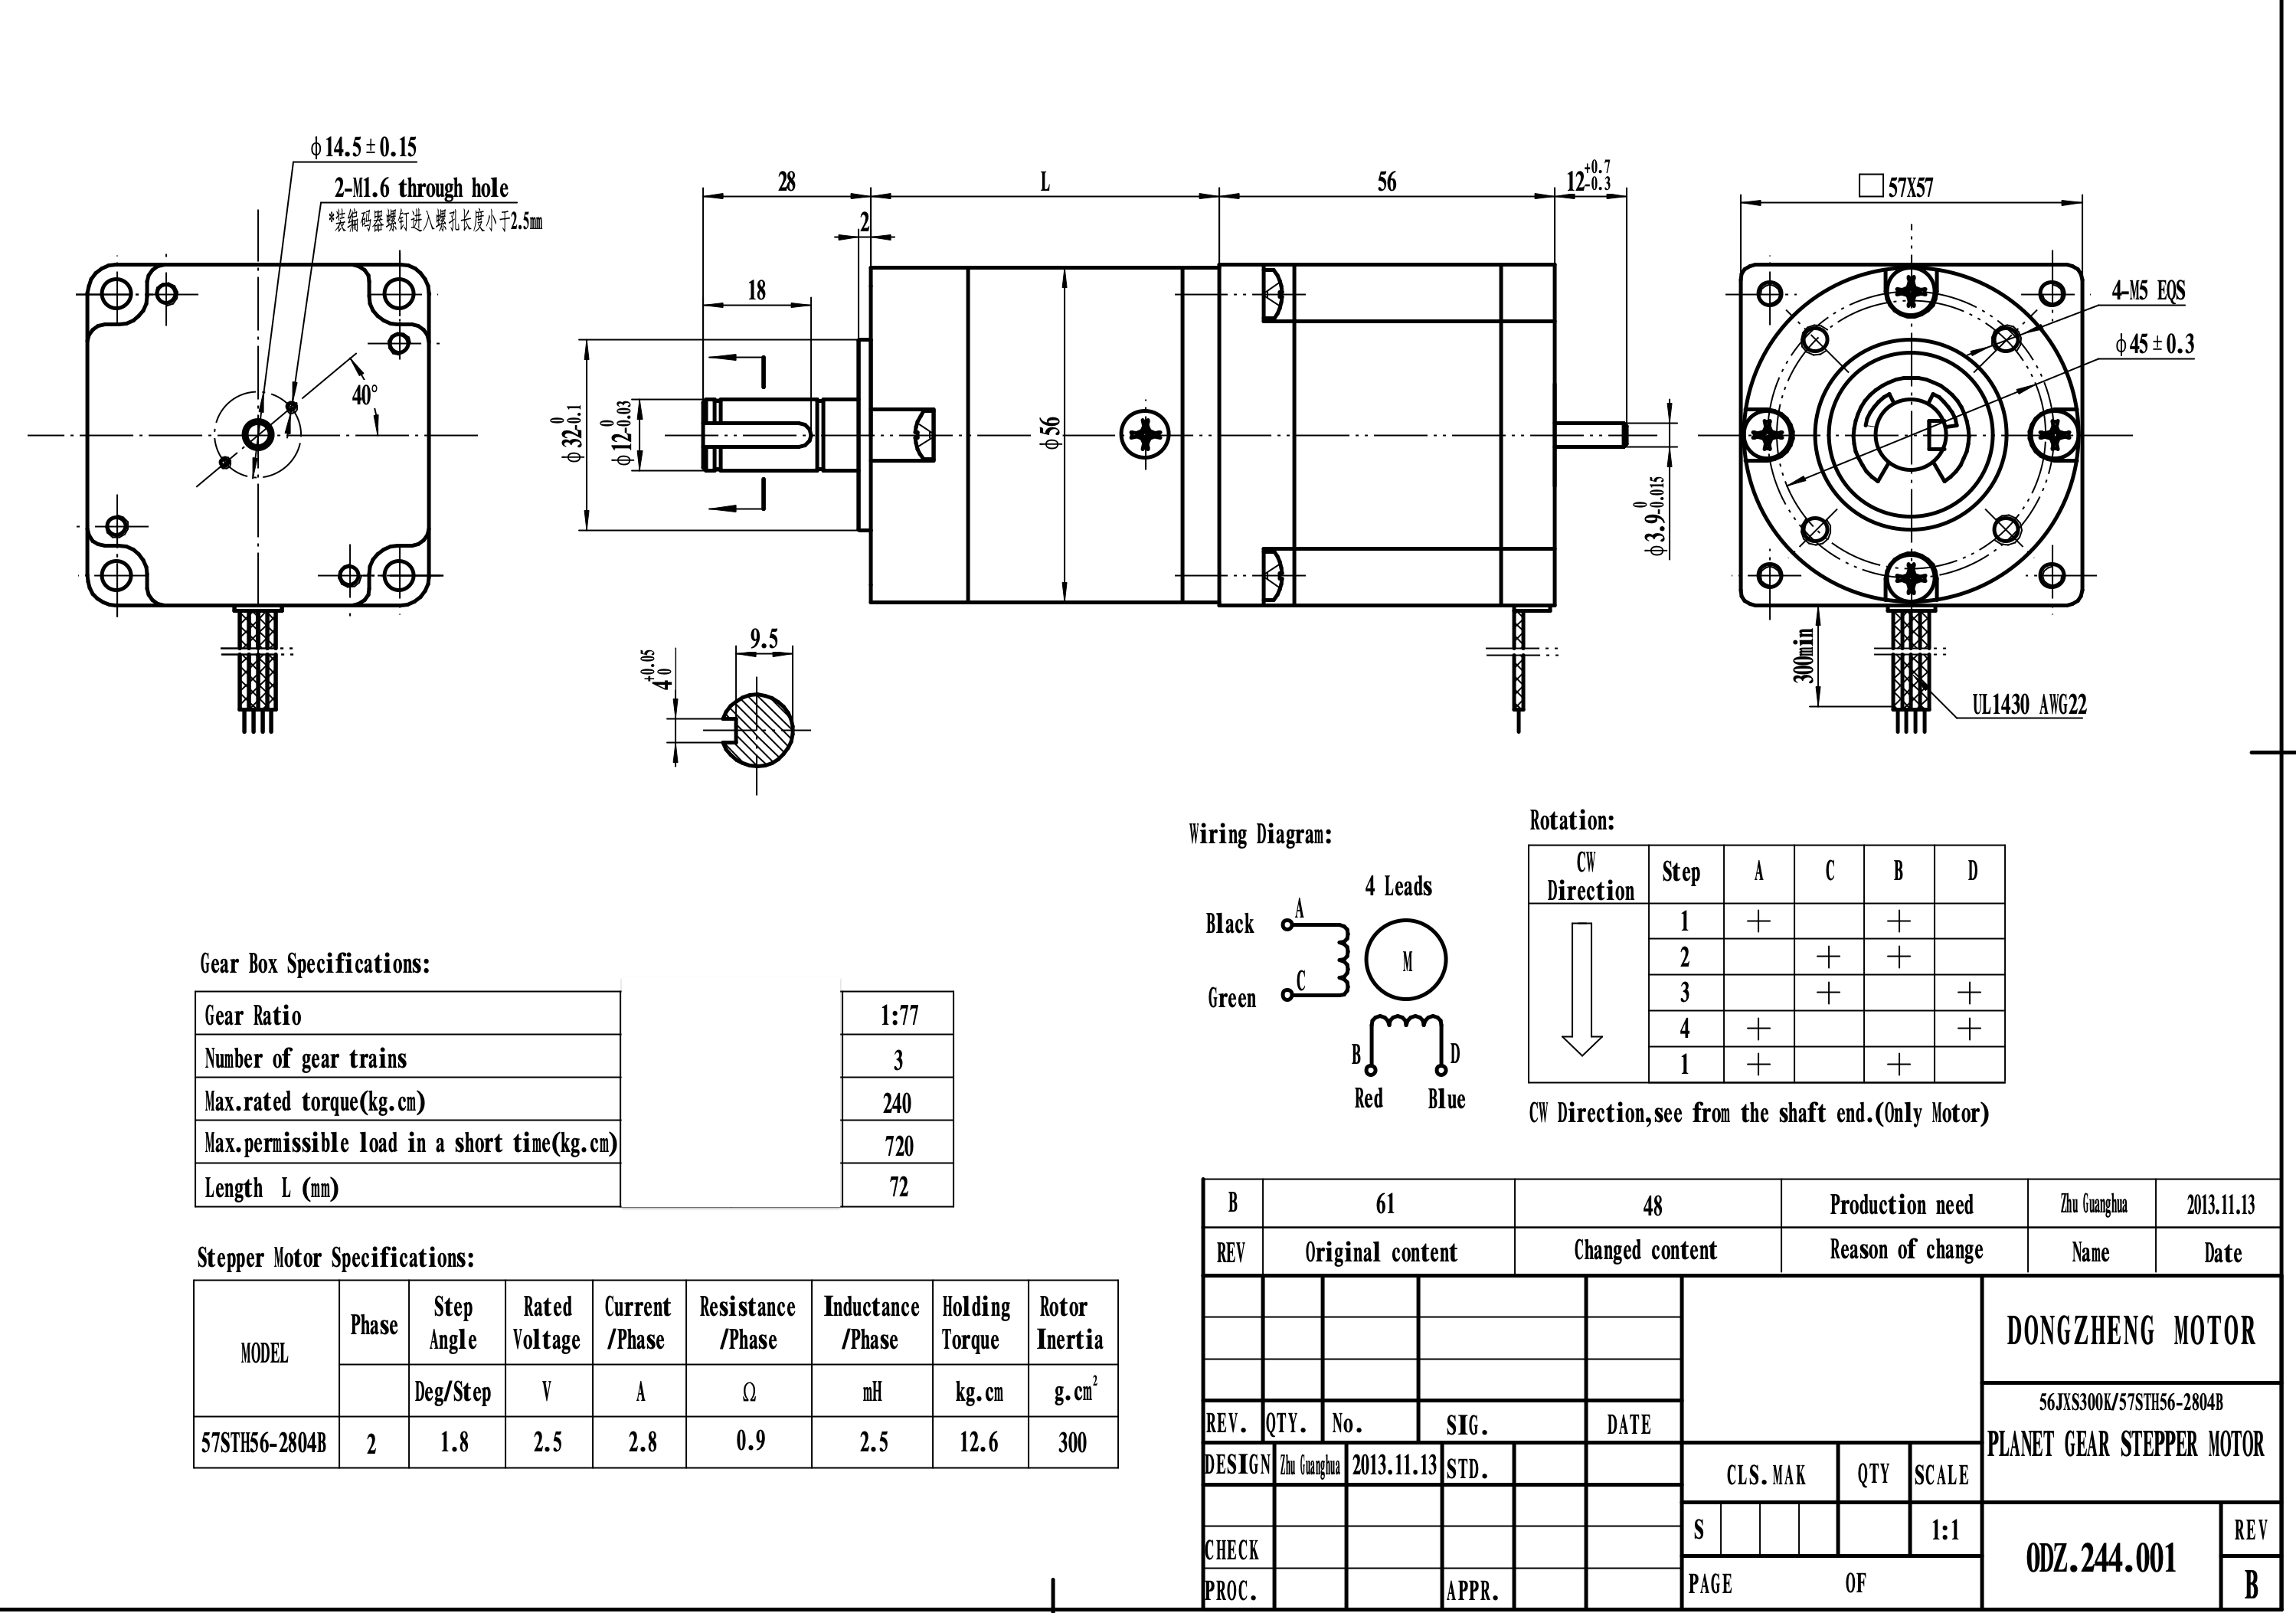
\includegraphics[width=0.6\textwidth]{Screen/STEPPER.png}
		\caption{Scheda tecnica dell'attuatore 57STH56 NEMA-23}
		\label{fig:Stepper}
	\end{figure}
	Il controllo dei motori passo-passo è molto semplice poichè possibile ad anello aperto, tramite l'uso di un controllore per la commutazione delle fasi ad onda quadra. Tutte le informazioni necessarie al collegamento meccanico ed elettrico sono state desunte dalla scheda tecnica in figura \ref{fig:Stepper} \\
	Il controllore scelto è il driver L6208 della STMicroelectronics, è un driver completamente integrato per motore passo-passo con protezione da sovracorrente. Il dispositivo include tutti i circuiti necessari per pilotare un motore passo-passo bipolare bifase: un doppio ponte DMOS completo, controller di corrente PWM a tempo di spegnimento costante che esegue la regolazione del taglio e della fase ed un generatore di sequenza che genera il passo. \\
	

	\begin{figure}
		\centering
		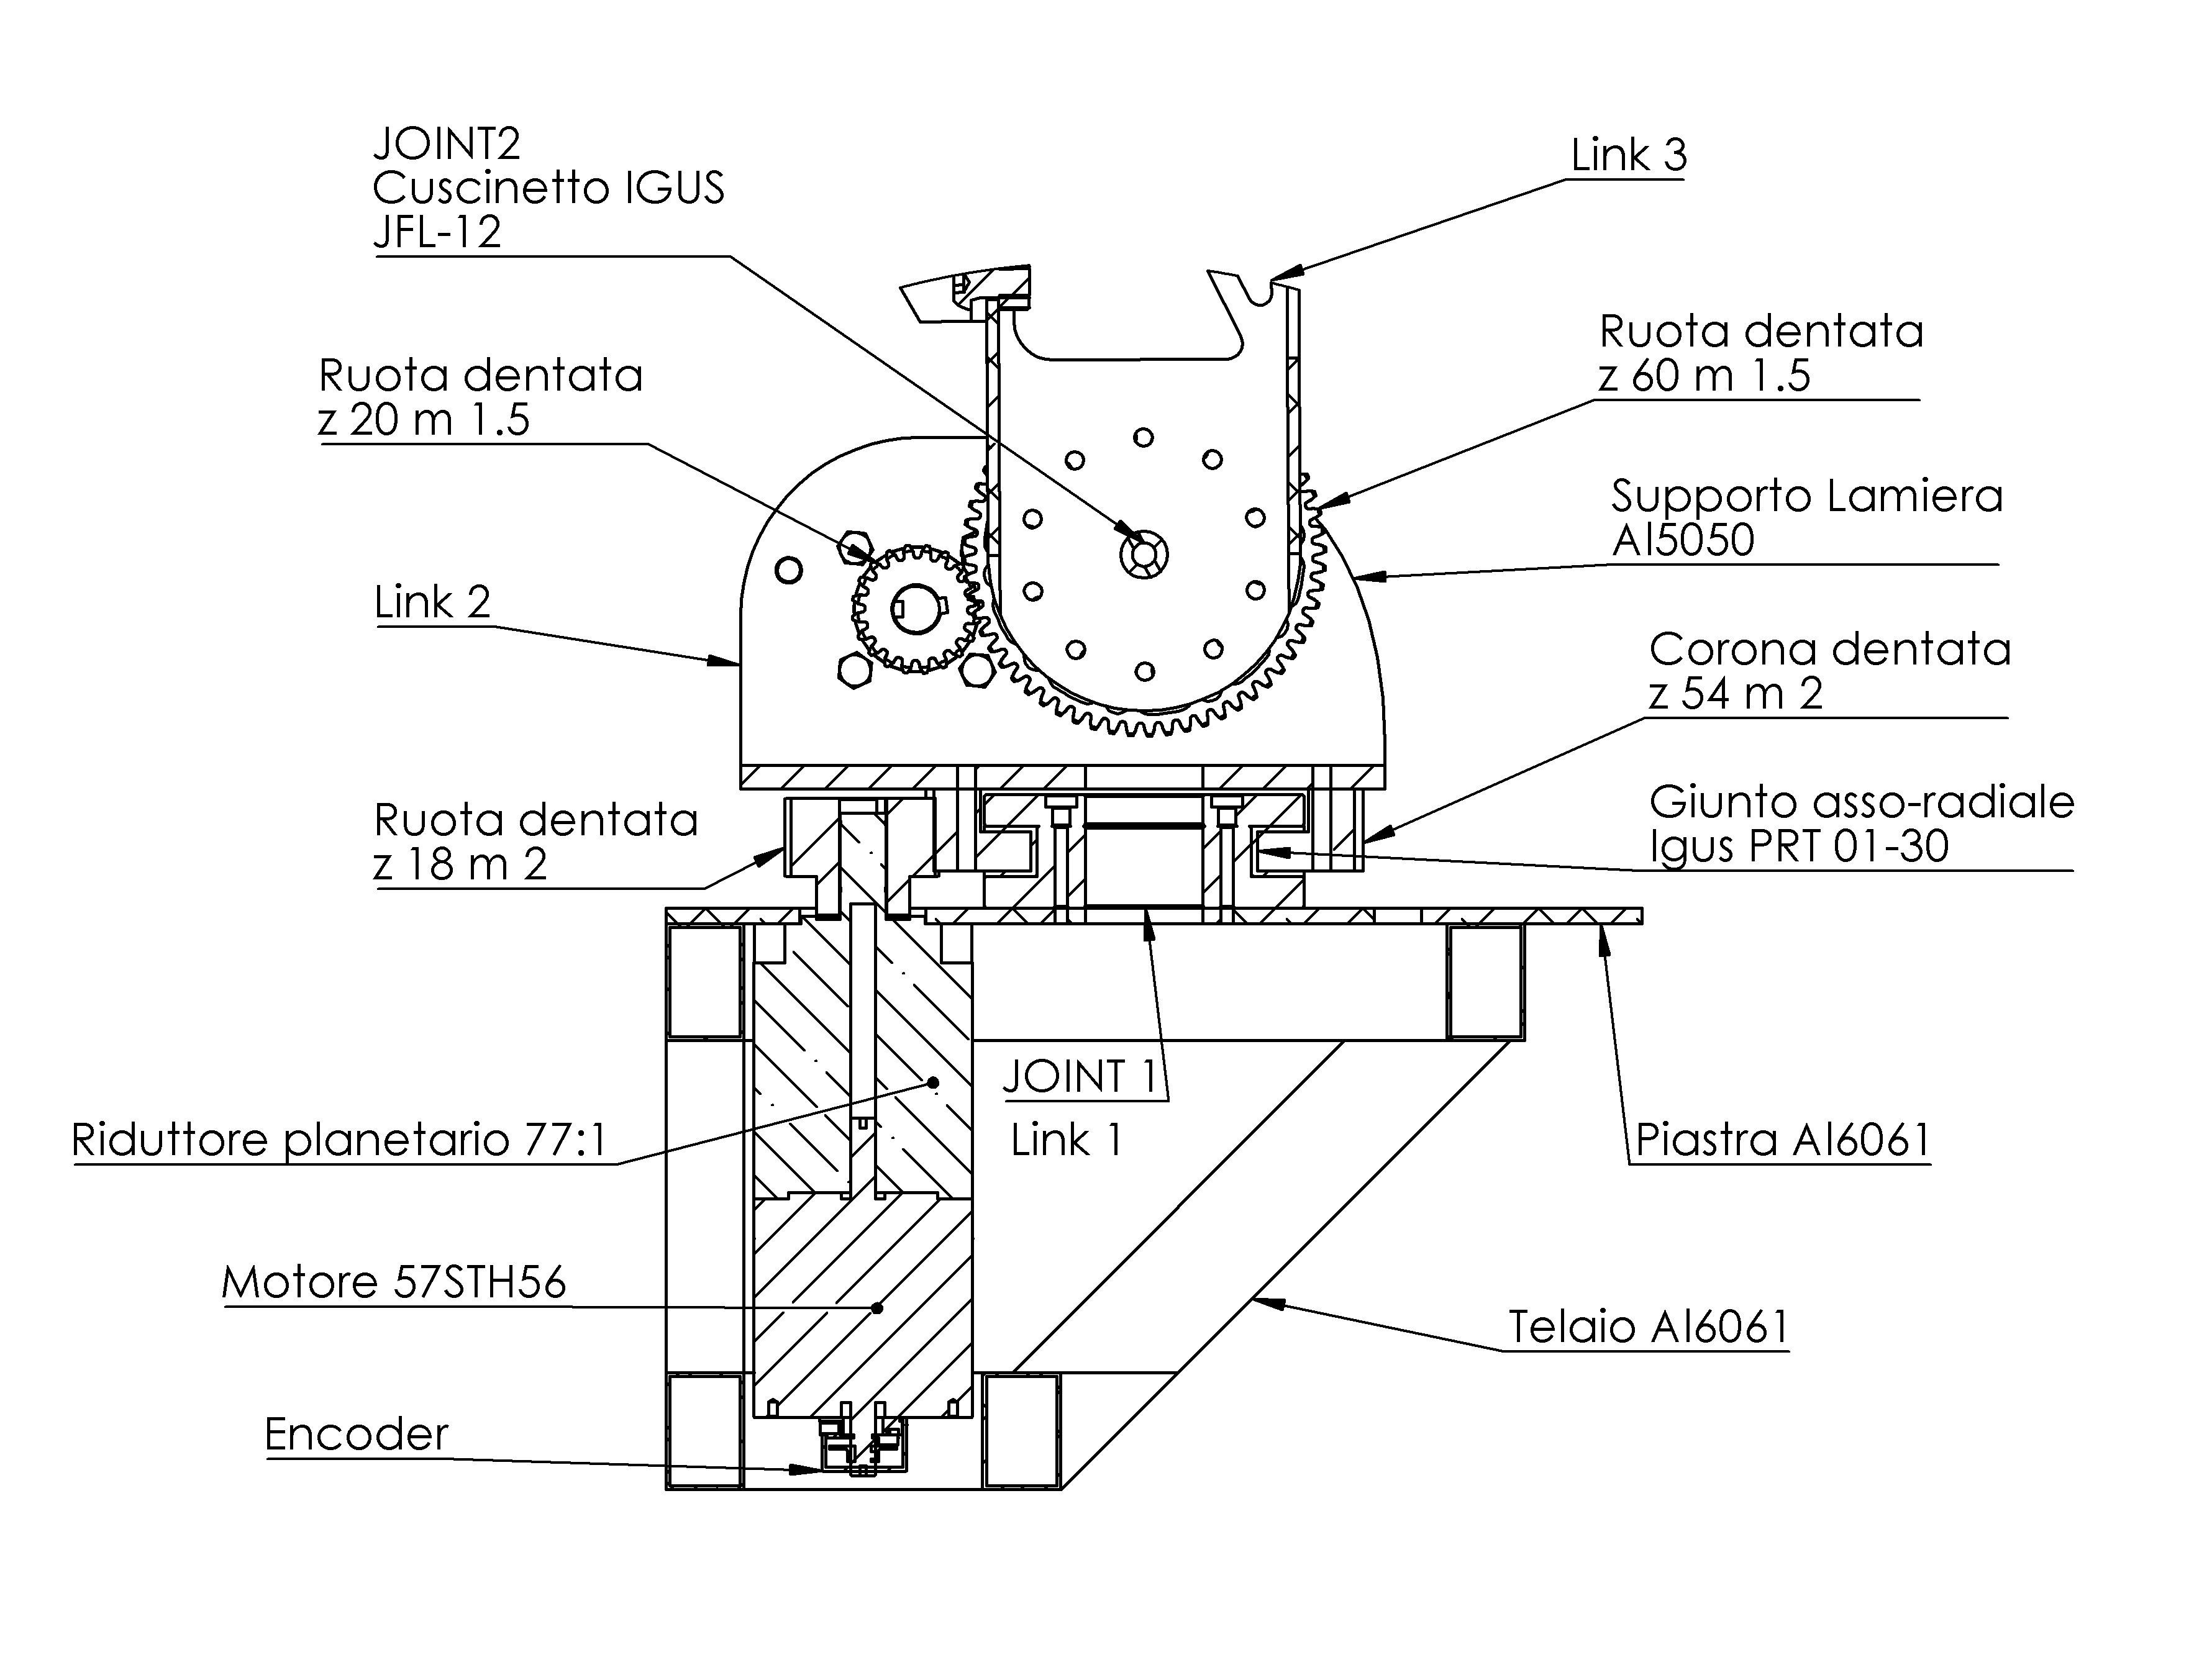
\includegraphics[width=\textwidth]{Screen/base.PNG}
		\caption{Schema della disposizione degli organi di trasmissione per i motori passo-passo}
		\label{fig:Stepper_cad}
	\end{figure}
		\subsection{Joint 1}
		\begin{figure}
			\centering
			\begin{tabular}{ll}
				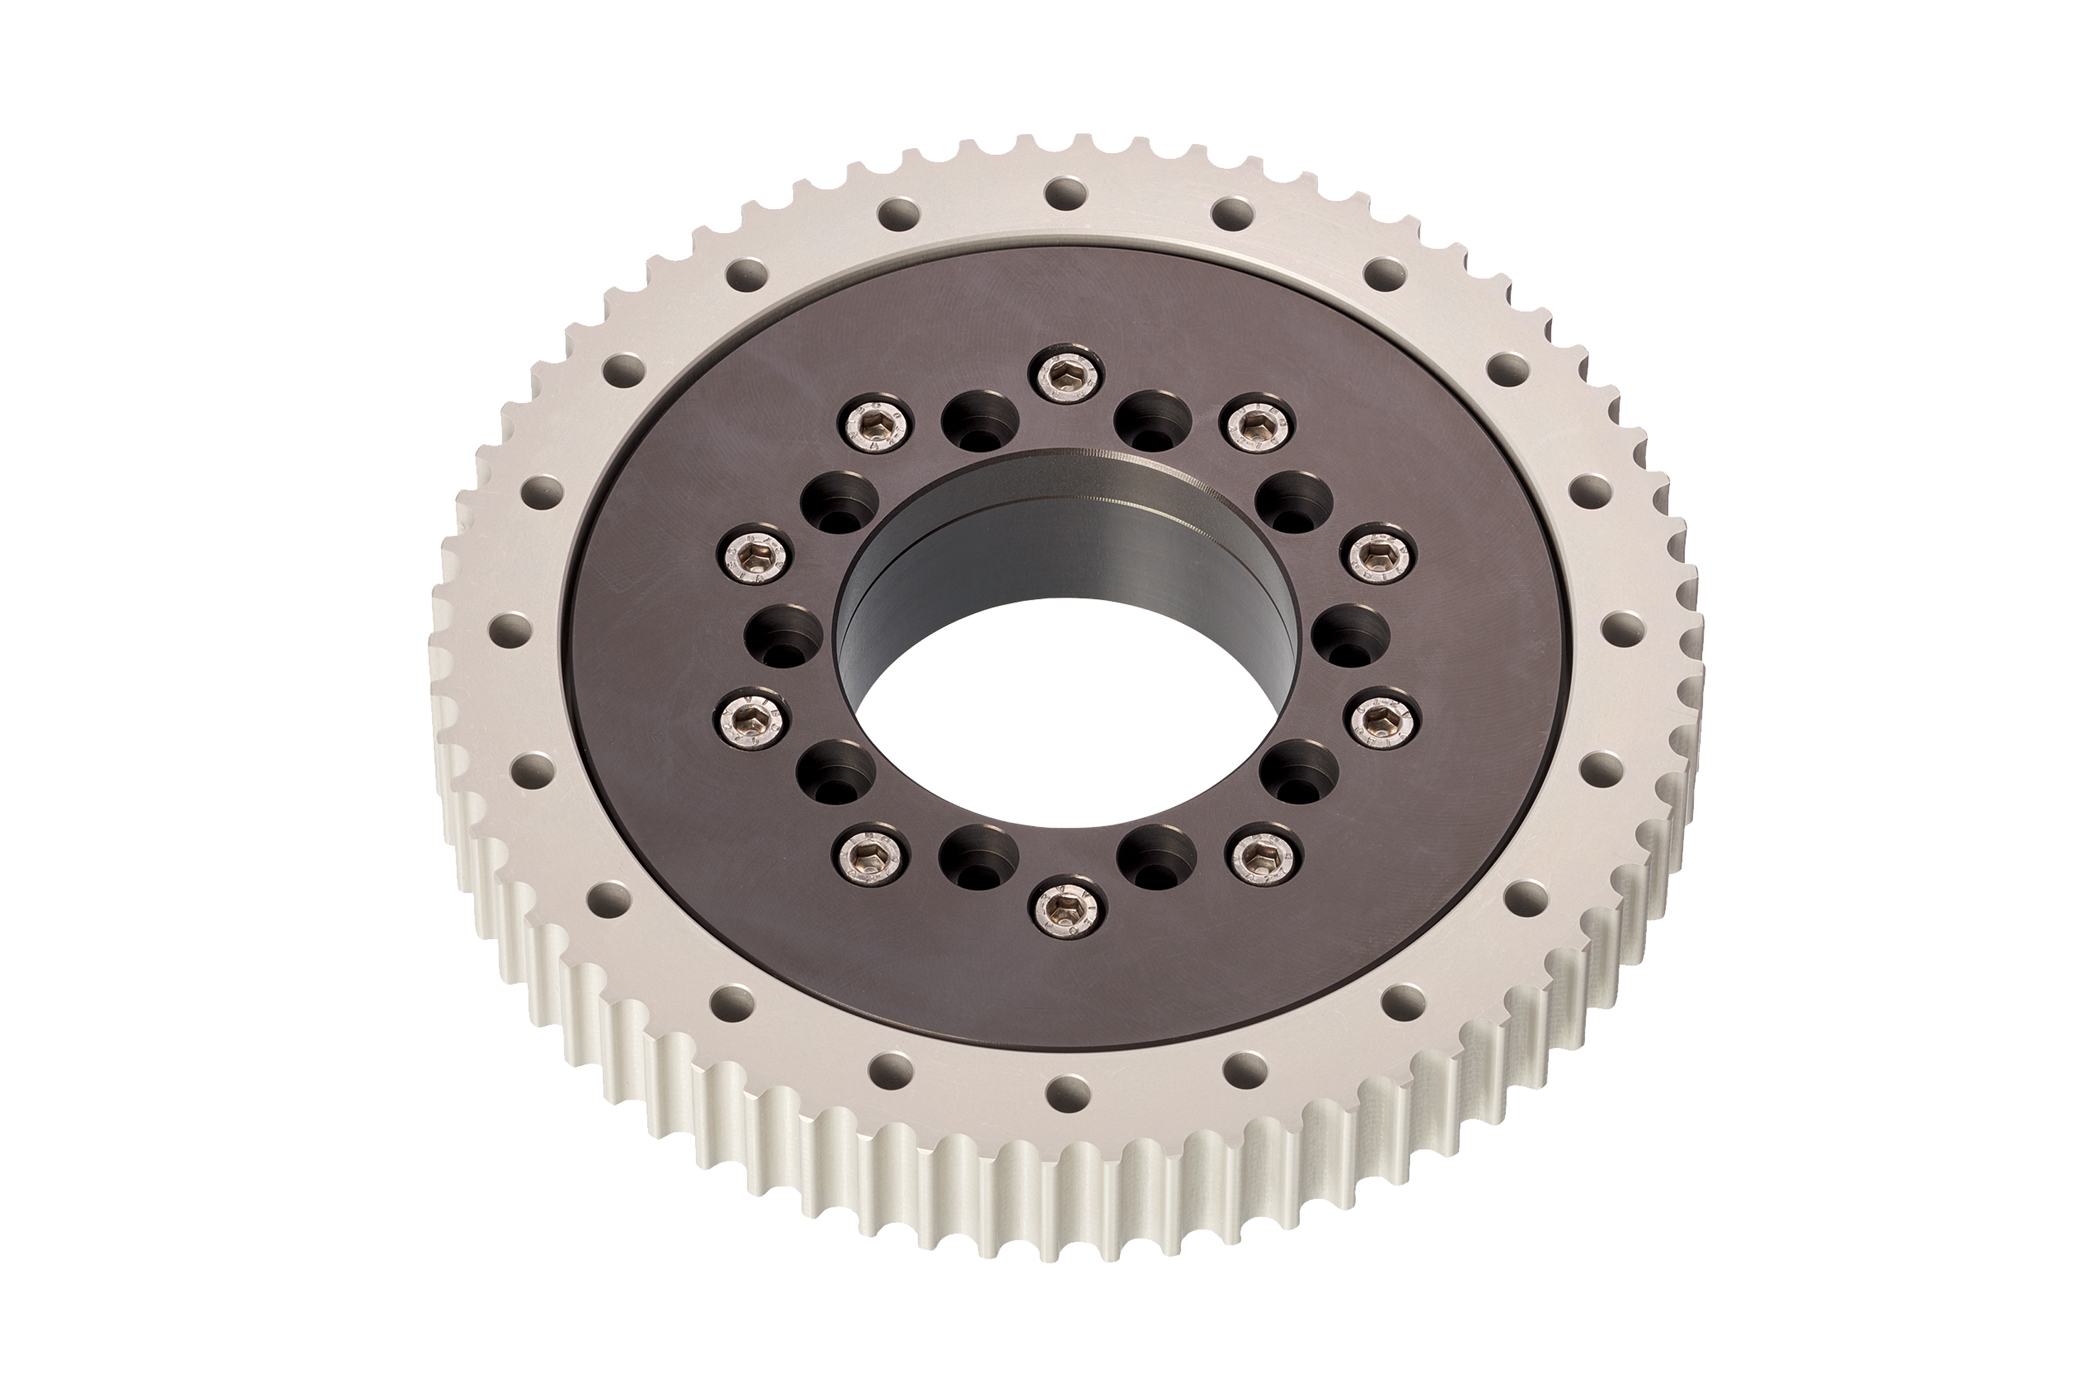
\includegraphics[height=4cm,keepaspectratio]{pictures/ralla.jpg}
				&
				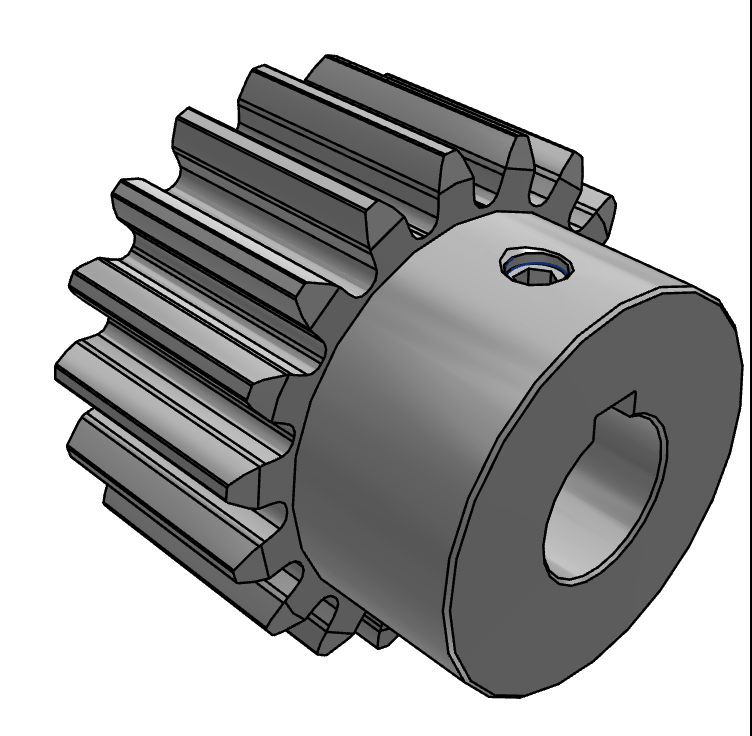
\includegraphics[height=4cm,keepaspectratio]{pictures/pignone.png}
			\end{tabular}
			\caption{Ralla IGUS PRT 01-30 e pignone MISUMI GEAKS2.0-18-20-B-12N}
			\label{fig:RALLA}
		\end{figure}
		Per il Joint 1, su cui ruota tutta la struttura del robot nel piano orizzontale, è necessario realizzare una base rigida su cui gravano il peso dell'intero robot ed un importante momento quando il braccio è completamente disteso e a sbalzo.\\
		 Perciò è stato impiegato un apposito giunto asso-radiale prodotto da IGUS, il \textit{PRT-01-30} in figura \ref{fig:RALLA}. \\
		La ralla IGUS è dotata di una corona esterna dentata di modulo unificato 2 mm e 54 denti perciò è stato possibile applicare un pignone prodotto da \textit{MISUMI codice GEAKS2.0-18-20-B-12N} al motoriduttore con 18 denti per realizzare un rapporto di riduzione 1 a 3. L'angolo di pressione è standard di 20° e la dentatura è a denti dritti. 
		\\
		\begin{tabular}{|c|c|c|c|c|c|c|c|}
			
			\hline
			Z1 & Z2 & Rapporto & a. pressione & a. elica & modulo & larghezza fascia & materiale \\
			\hline
			18 & 54 & 1/3 & 20° & 0°  & 2 & 20 mm & C45  \\
			\hline
			
		\end{tabular}
		\\
		Si assume che la dentatura di modulo 2 mm in acciaio sia in grado di trasmettere la potenza prodotta dal motoriduttore con ampio margine di sicurezza, pertanto non è stata dimensionata ma sono state verificate le forze scambiate dal modello multibody in figura \ref{fig:MBDforze1}. \\
		Dal modello multibody sono state misurati due set di dati: quelli relativi alla ralla e quelli relativi all'attuazione. \\
		In figura possiamo valutare la coppia richiesta all'attuatore dalla trasmissione con rapporto di riduzione 1 a 3 per realizzare una rotazione della base con il braccio in posizione distesa e ritratta, evidenziando l'impatto della posizione del braccio sulla prestazione del motore. \\
		Il modello tiene conto dell'attrito opposto dalla cerniera avendo inserito nel modello di simulazione il corretto valore di coefficiente di attrito dinamico fornito dalla produttrice IGUS pari a 0.2. 
		
		Condizioni di simulazione :
		\begin{itemize}
			\item Traiettoria svolta nella condizione favorevole: il braccio si chiude e il giunto compie una rotazione di 90° 
			\item Traiettoria svolta nella condizione sfavorevole: il braccio si distende e il giunto compie una rotazione di 90° 
			\item Velocità dell'attuatore 1 rpm
			\item Payload : massa concentrata di 5kg nel TCP 
		\end{itemize}

		\begin{figure} [!ht]
			\centering
			\begin{tabular}{ll}
				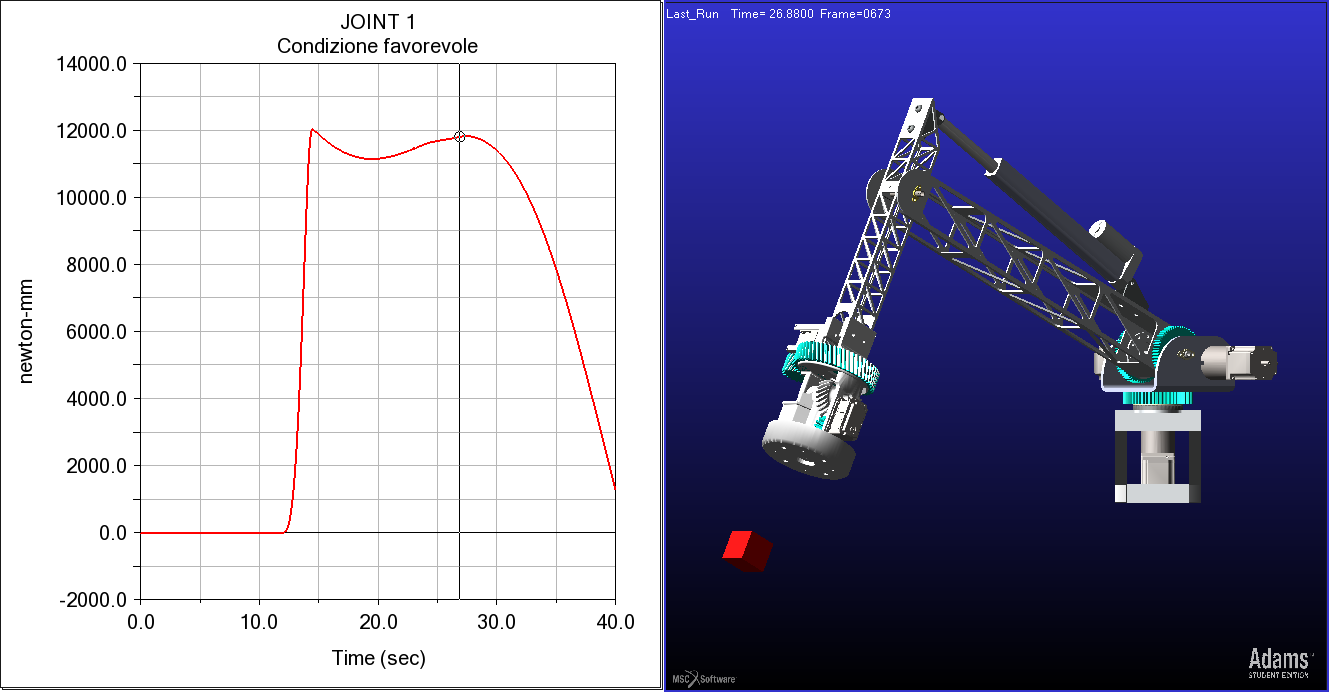
\includegraphics[height=4cm,keepaspectratio]{Plots/BASE/joint1_FAVOREVOLE.png}
				&
				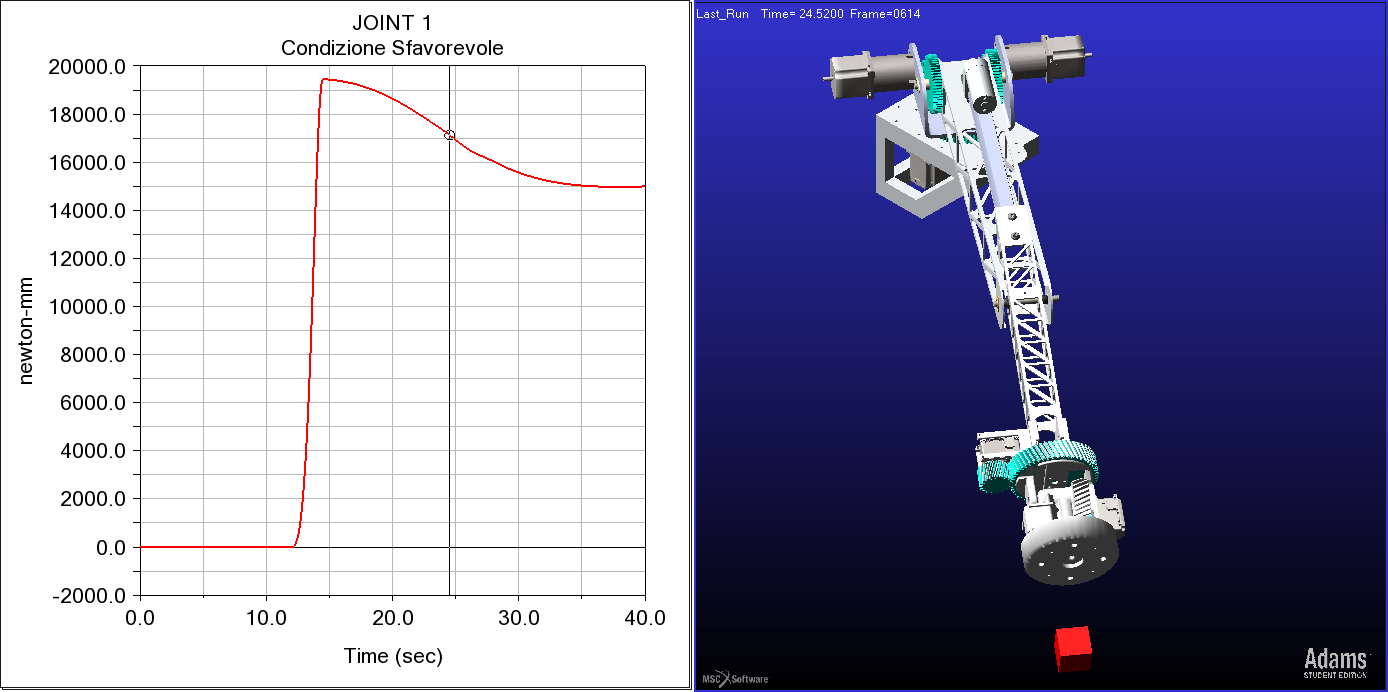
\includegraphics[height=4cm,keepaspectratio]{Plots/BASE/joint1_sfavorevole.png}
			\end{tabular}
			\caption{Coppia richiesta al motore per attuare la rotazione della base con braccio disteso e ritratto}
			\label{fig:MBDcoppia1}
		\end{figure}
	
	\begin{figure} [!ht]
		\centering
		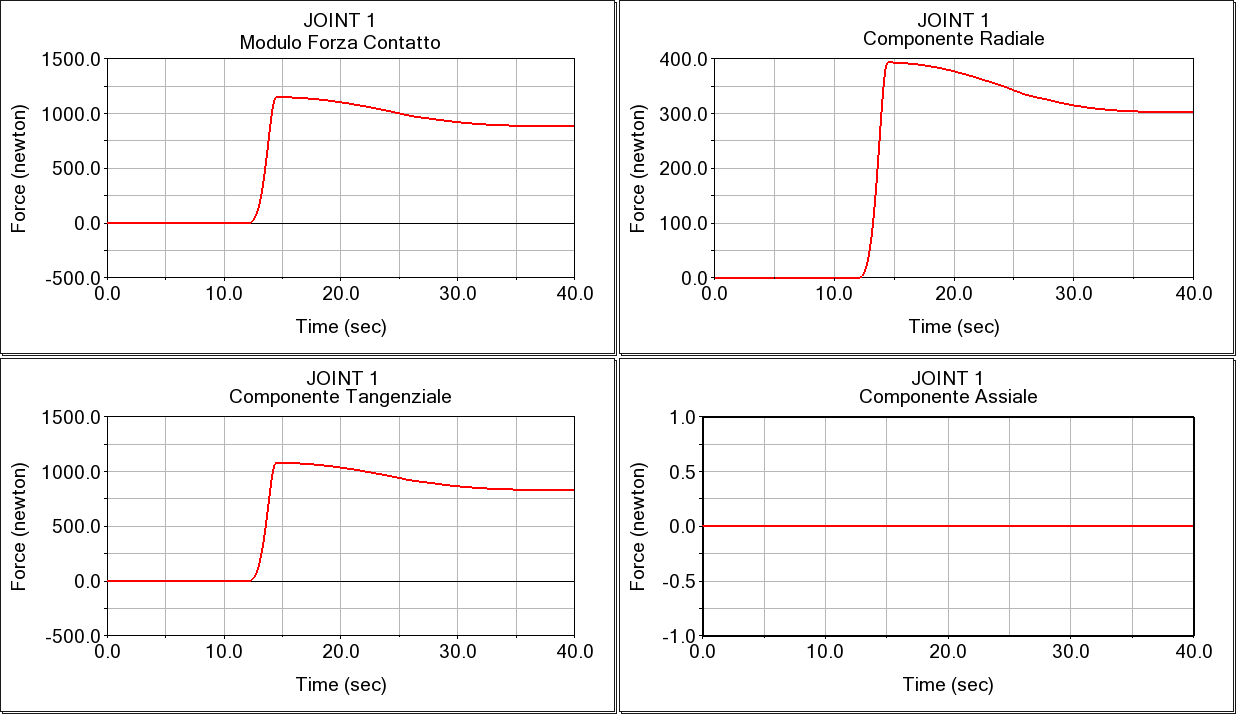
\includegraphics[width=0.6\textwidth]{Plots/BASE/joint1_forze.png}
		\caption{Forze scambiate nell'ingranamento}
		\label{fig:MBDforze1}
	\end{figure}
	\begin{figure}[!ht]
		\centering
		\includegraphics[width=0.6\textwidth]{Plots/BASE/joint1_ralla.png}
		\caption{Momento di ribaltamento sul giunto e forza assiale nella configurazione più sfavorevole}
		\label{fig:MBDralla1}
	\end{figure}
	
			Dai dati raccolti si evidenzia che nella condizione più sfavorevole in figura \ref{fig:MBDcoppia1}  ci si avvicina al valore di coppia massima prevista per l'attuatore con un valore di 20 Nm senza comunque superarla mentre nella condizione favorevole si è ben al di sotto con massimo di 12 Nm. \\
			Pertanto si prevede che l'attuatore sarà in grado di movimentare il carico senza che perda passi e che si crei quindi uno shift tra la posizione attesa e quella effettivamente raggiunta. Questa condizione può essere comunque recuperata dalla presenza di un encoder che registri la posizione effettivamente raggiunta. \\
			
			Successivamente è necessario verificare che il componente scelto per la cerniera possa sopportare i carichi imposti dal meccanismo quando si trova nella condizione più sfavorevole.\\
			Dai dati raccolti in figura \ref{fig:MBDralla1} il carico assiale massimo è inferiore ai 7000 N previsti dalla scheda tecnica e il momento massimo è inferiore ai 200 Nm previsti. Pertanto il componente è sicuramente in grado di sopportare i carichi imposti dal robot garantendo l'assenza di gioco nella trasmissione. \\
			
	
	
		\subsection{Joint 2}
		\begin{figure}
			\centering
			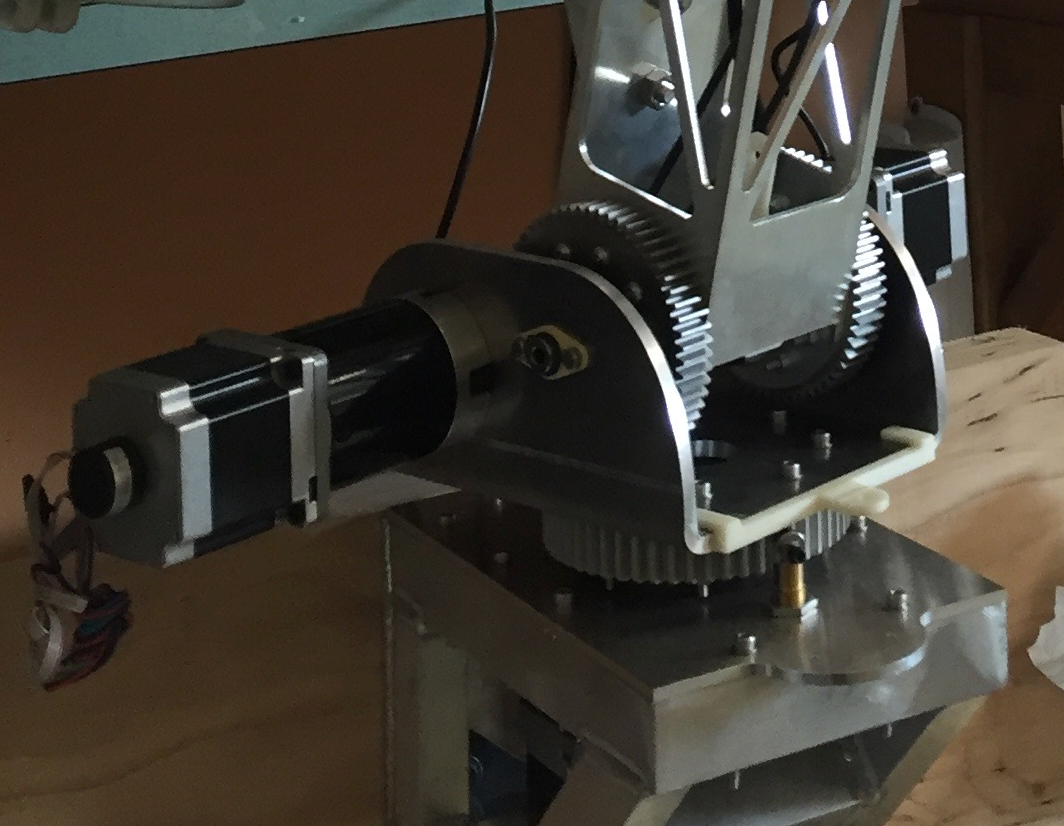
\includegraphics[width=0.4\textwidth]{image/basefoto.png}
			\caption{Disposizione dei motori passo-passo e della ruota condotta flagiata al link 3}
			\label{fig:Stepper_foto}
		\end{figure}
	
		\begin{figure}[!ht]
			\centering
			\begin{tabular}{ll}
				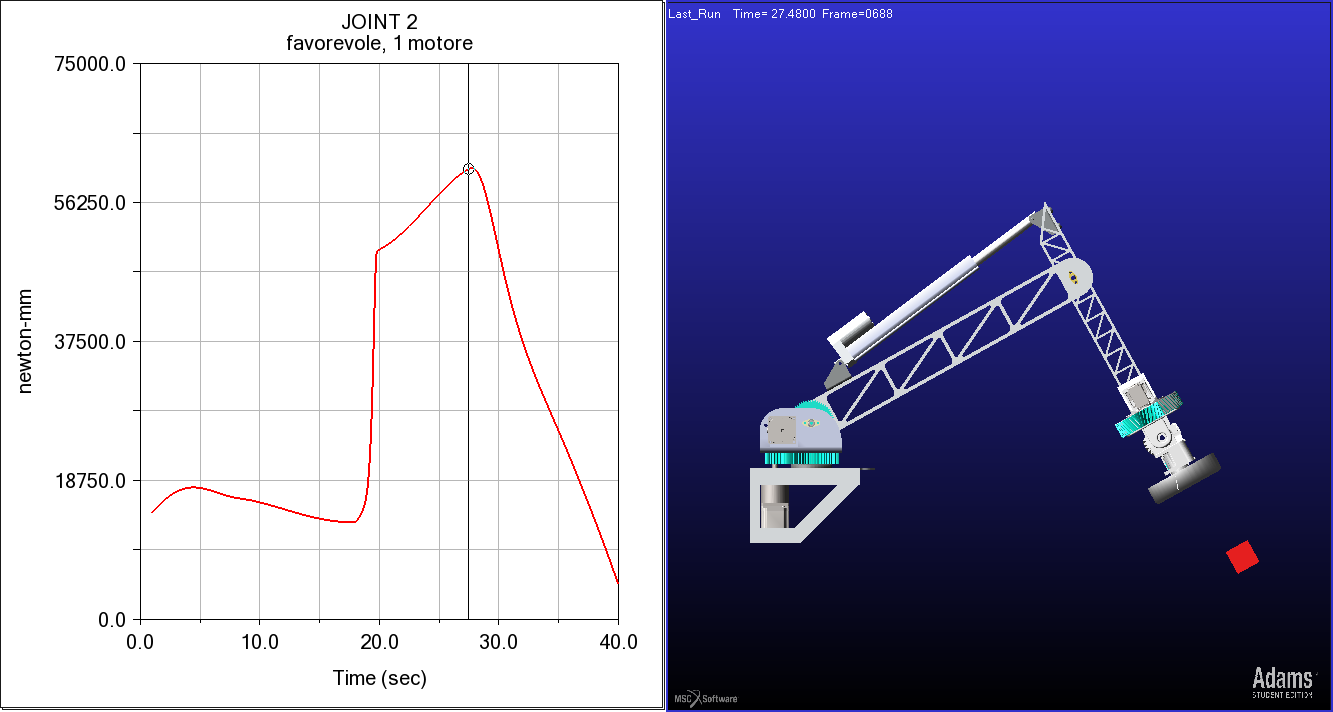
\includegraphics[height=4cm,keepaspectratio]{Plots/SPALLA/1motore/JOINT2_conservativo.png}
				&
				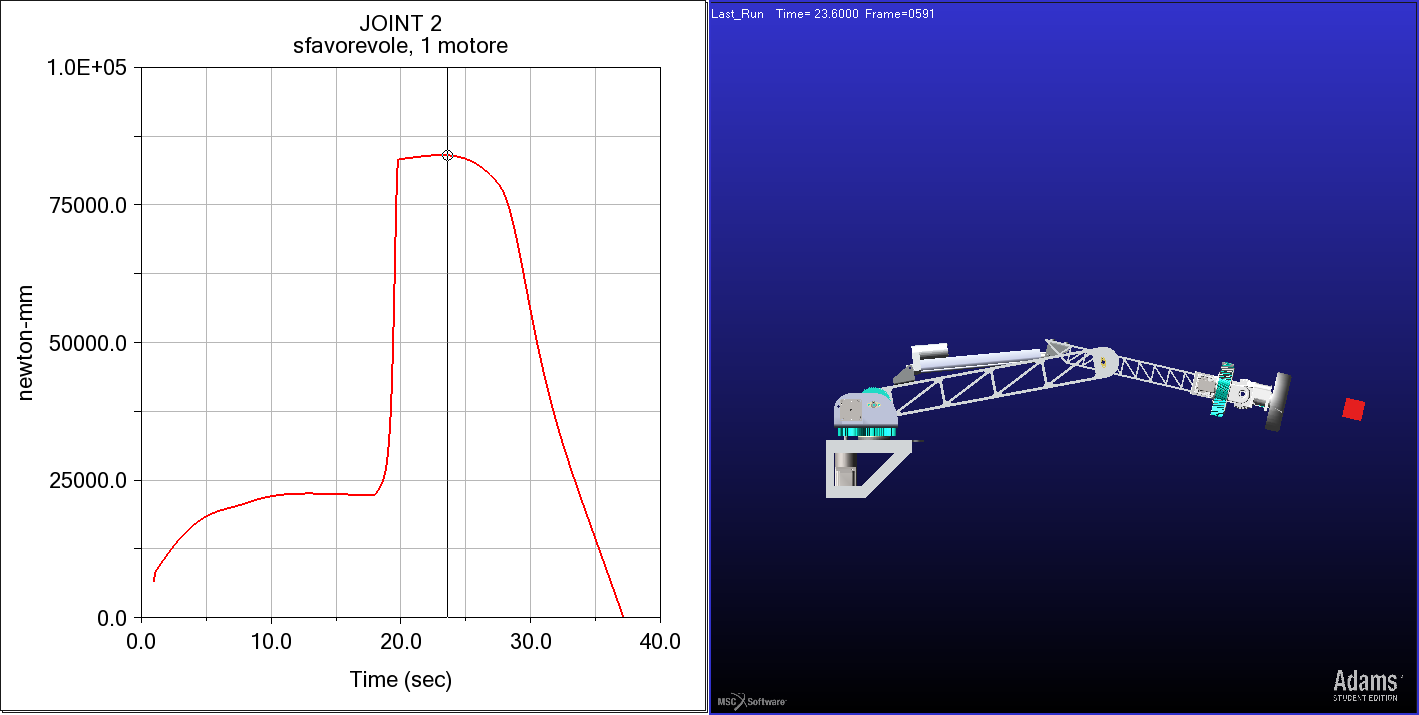
\includegraphics[height=4cm,keepaspectratio]{Plots/SPALLA/1motore/JOINT2-torque.png}
			\end{tabular}
			\caption{Valori di coppia richiesti nel caso in cui ci fosse un solo attuatore}
			\label{fig:MBDJoint21motore}
		\end{figure}
		\begin{figure} [!ht]
			\centering
			\begin{tabular}{ll}
				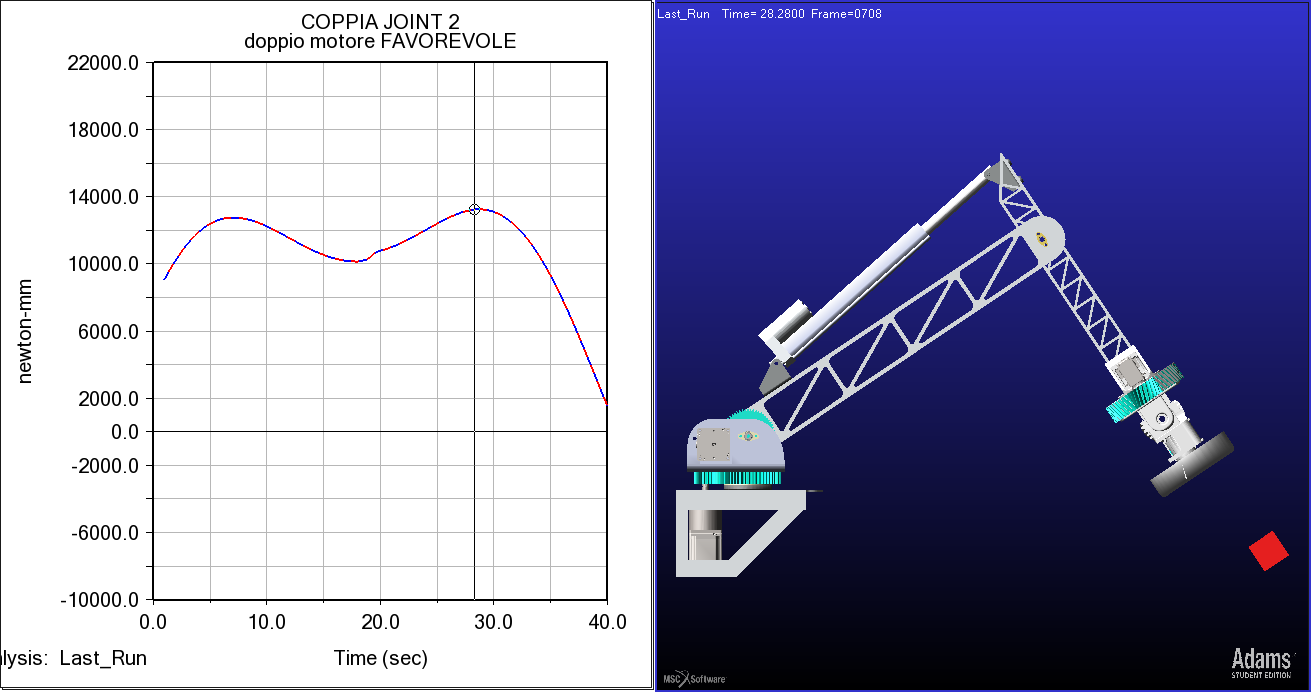
\includegraphics[height=4cm,keepaspectratio]{Plots/SPALLA/2motori/JOINT22favorevole.png}
				&
				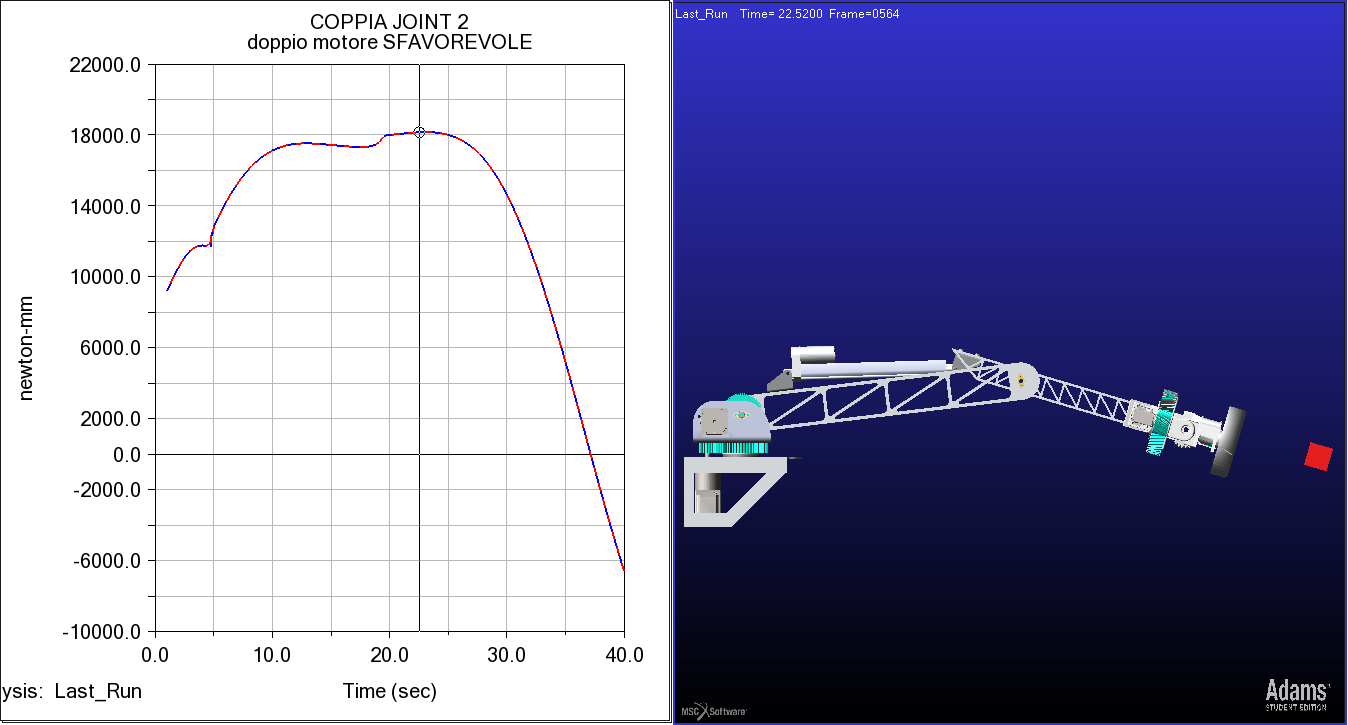
\includegraphics[height=4cm,keepaspectratio]{Plots/SPALLA/2motori/JOINT22sfavorevole.png}
			\end{tabular}
			\caption{Valori di coppia richiesti con due attuatori gemellati}
			\label{fig:MBDJoint22motore}
		\end{figure}
		Per il Joint 2 sono stati scelti gli stessi motoriduttori mostrati precedentemente, montati in configurazione gemellata che si vede in figura \ref{fig:Stepper_foto}. \\
		Questa soluzione si è resa necessaria in quanto un solo attuatore non è sufficiente a garantire la coppia necessaria come mostrato in figura \ref{fig:MBDJoint21motore} e per realizzare una simmetria delle coppie di reazione che si scaricano sulla struttura del Link 1. \\
		
		
		I due attuatori trasmettono il moto al Link 1 mediante ruote dentate flangiate sulla struttura ed erogano potenza lavorando in parallelo. Ciò permette inoltre di non caricare a torsione la trave del Link 1 visto che i carichi risultano simmetrici. 
		
		Nella soluzione con 2 attuatori come si vede in figura \ref{fig:MBDJoint22motore} le prestazioni del motore sono sufficienti a movimentare il carico. Nel grafico è rappresentata la coppia erogata dal singolo motore.\\
		Il modello multibody anche in questa fase si è rivelato fondamentale al fine di fornire dei carichi verosimili da applicare all'analisi strutturale e nell'ottimizzazione della struttura da parte del team di analisi FEM. 
		\\
			Condizioni di simulazione :
		\begin{itemize}
			\item Traiettoria svolta nella condizione favorevole: il braccio si chiude e il giunto compie una rotazione di 90° 
			\item Traiettoria svolta nella condizione sfavorevole: il braccio si distende e il giunto compie una rotazione di 90° 
			\item Velocità dell'attuatore 1 rpm
			\item Payload : massa concentrata di 5kg nel TCP 
		\end{itemize}
		L'attuatore trasferisce il moto al Link 3 del braccio mediante un ingranamento tra ruote dentate a denti dritti di modulo 1,5 e rapporto di riduzione 3. Al motoriduttore è applicato un pignone da 20 denti \textit{MISUMI GEAKS1.5-20-15-B-12N} e al link 3 una ruota condotta da 60 denti \textit{GEAKS1.5-60-15-A-12N} con larghezza di fascia 15mm. \\
		
			\begin{tabular}{|c|c|c|c|c|c|c|c|}
			
			\hline
			Z1 & Z2 & Rapporto & a. pressione & a. elica & modulo & larghezza fascia & materiale \\
			\hline
			20 & 60 & 1/3 & 20° & 0°  & 1,5 & 15 mm & C45  \\
			\hline
			
		\end{tabular}
		\\
		\\
		L'ingranamento non è stato dimensionato in quanto si ritiene sicuramente verificato per la potenza in gioco  ruota condotta applicata al link 3 offre un perfetto compromesso dimensionale per poterla flagiare direttamente sul link 3 come si vede in figura \ref{fig:Stepper_foto} con una corona di viti, in modo da non richiedere un albero di trasmissione, una cartella o la realizzazione di sedi linguetta sulla sottile trave in alluminio che aveva evidenziato una forte criticità dal punto di vista strutturale e di concentrazione degli sforzi. \\
		
		\begin{figure} [!ht]
		\centering
			\begin{tabular}{ll}
				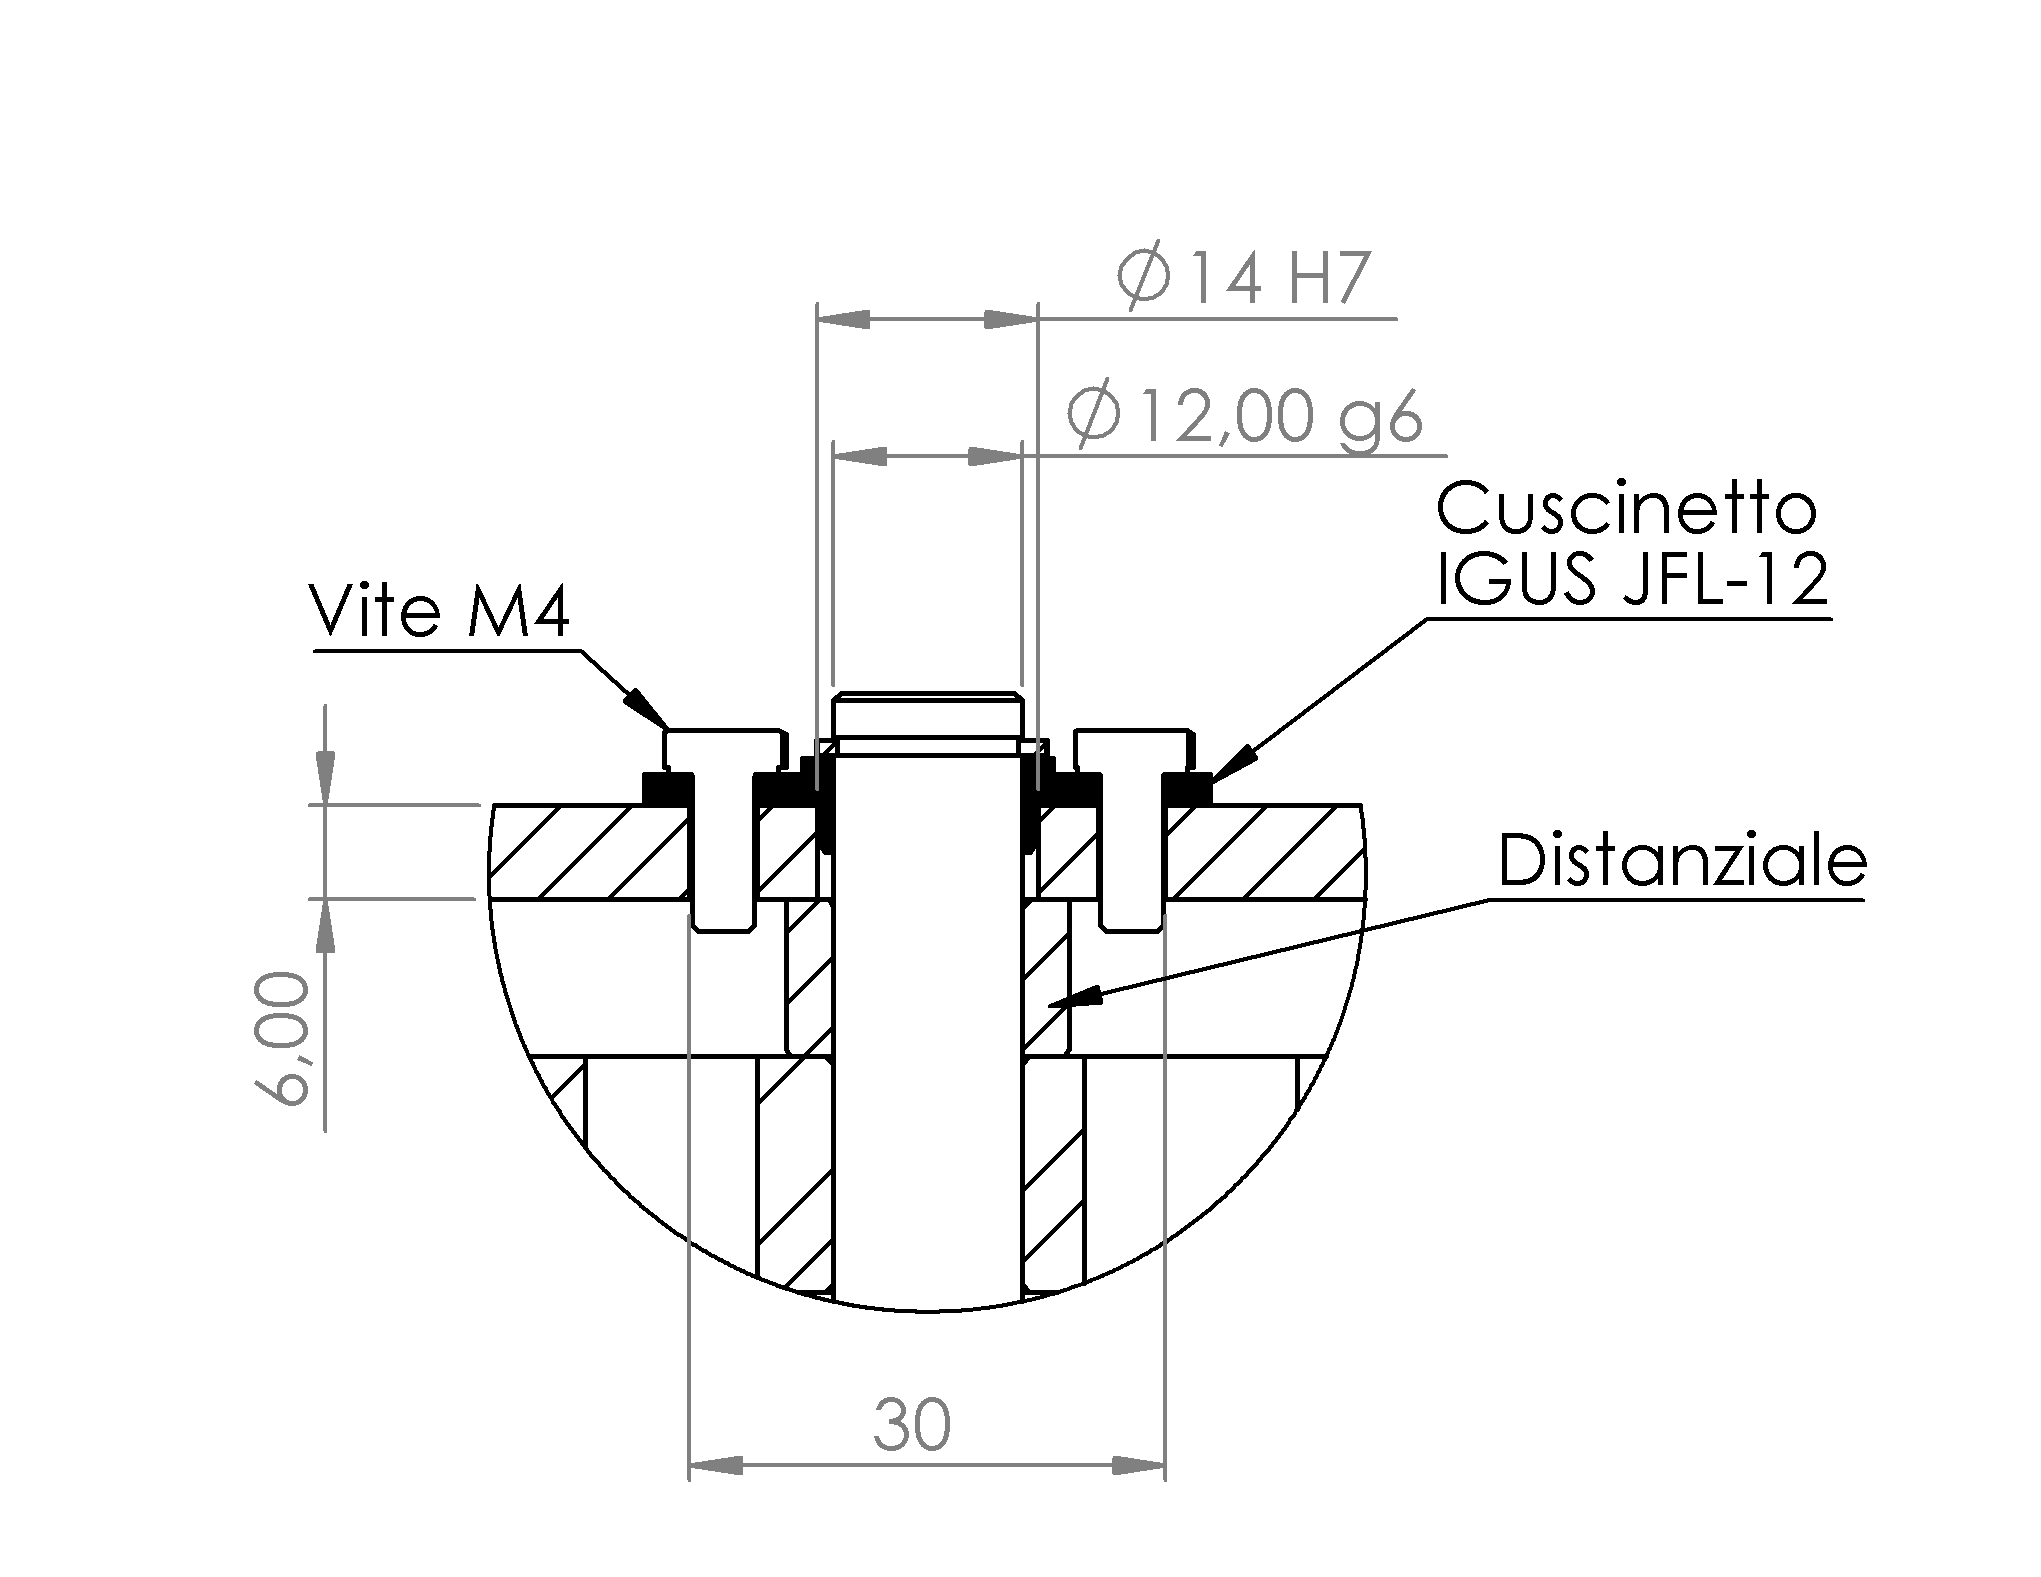
\includegraphics[width=0.4\textwidth]{Screen/cuscinetto.png}
				&
				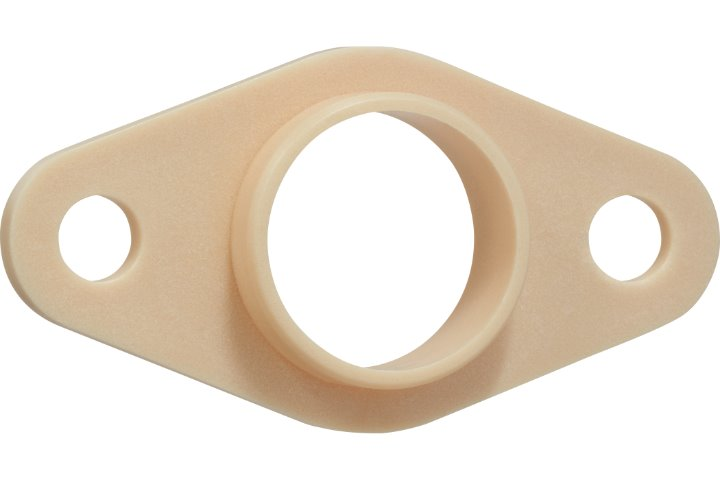
\includegraphics[width=0.4\textwidth]{image/jfl12.jpg}
			\end{tabular}				
		\caption{Dettaglio del cuscinetto del Joint 2}
		\label{fig:cuscinetto_foto}
		\end{figure}		
		
		La cerniera del Joint 2 è composta da due cuscinetti senza corpi volventi flangiati \textit{IGUS JFL-12} che possono essere usati per realizzare una sede calibrata per albero in tolleranza standard quando applicati all'interno di un foro calibrato su lamiera, senza richiedere lavorazioni aggiuntive o una cartella. Un dettaglio si trova in figura \ref{fig:cuscinetto_foto}.
	
		
	
	
	\section{Attuatori Lineari, Cinematismo Joint 3}
	
	Nella scelta dell'attuatore per il Joint 3 è rilevante non solo la potenza richiesta ma anche il peso del componente. Difatti, lo svantaggio degli attuatori passo-passo precedentemente descritti è sicuramente il rapporto tra peso del componente e potenza erogata che risulta sfavorevole.\\
	Per il Joint 3 la scelta di un attuatore rotativo sufficientemente potente da collocare sull'asse del giunto avrebbe peggiorato fortemente le proprietà inerziali del Link 3, collocando una massa importante concentrata in punta alla trave. \\
	Nei robot industriali questo problema viene aggirato collocando i motori alla base dei link e trasmettendo potenza meccanica ad alta velocità di rotazione tramite una cinghia contenuta all'interno della trave e collocando un riduttore epicicloidale o armonico dotato di encoder coassiale al giunto. \\
	Per risolvere questo problema si è optato per una soluzione alternativa e non convenzionale nel campo dei robot industriali. 
	\\
	La scelta di un attuatore lineare, un componente molto economico e di larga diffusione nelle forniture di automazione, ha permesso di posizionare l'attuatore e quindi la sua massa molto in basso e non appensantendo il link 3. \\
		\begin{figure}
		\centering
		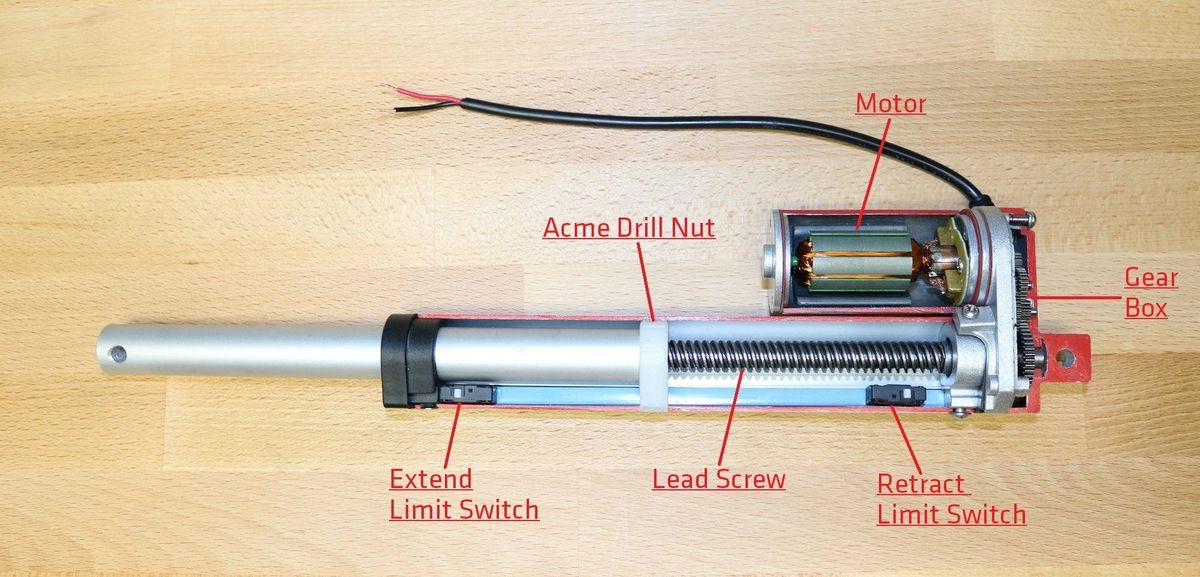
\includegraphics[width=0.4\textwidth]{image/linearact.jpg}
		\caption{Interno di un attuatore lineare del tipo scelto nel progetto }
		\label{fig:linearact}
	\end{figure}
	Gli attuatori lineari di questo tipo sono generalmente costituiti da un motore in corrente continua a spazzole, un riduttore ed una trasmissione vite-madrevite che trasforma il moto rotativo in uscita dal motore in traslazione lungo un giunto prismatico come si vede in figura \ref{fig:linearact}.\\
	L'attuatore è inoltre dotato di interruttori di fine corsa che ne limitano il moto all'escursione prevista. Il sistema di controllo è molto semplice: essendo fondamentalmente un motore in corrente continua, è sufficiente invertire i contatti al fine di invertire la direzione del moto.\\ 
	Per pilotare l'attuatore è stato scelto un driver per motori DC di STMicroelectronics, l'integrato L6206 che include in un solo componente un ponte H a semiconduttori, una pompa di carica per pilotare i MOSFET che costituiscono il ponte e la logica di controllo necessaria a realizzare anche un pilotaggio PWM per avere velocità variabili e il funzionamento nei 4 quadranti della caratteristica elettrica del motore. 
	
	I parametri progettuali che è necessario determinare per la scelta dell'attuatore sono :
	\begin{itemize}
		\item La lunghezza dell'attuatore completamente ritratto e la corsa necessaria per rispettare il workspace calcolato
		\item La posizione delle cerniere di ancoraggio e la lunghezza del braccio di leva su cui agisce l'attuatore
		\item La forza necessaria per movimentare il carico 
		\item La velocità di traslazione massima 
	\end{itemize}
	
	Lo studio cinematico, quindi delle lunghezze e della posizione delle cerniere è stato sviluppato grazie al modello multibody. Una caratteristica centrale di questi modelli è la parametrizzazione.\\
	 Grazie alla possibilità di parametrizzare alcune variabii che costituiscono il modello si può svolgere un esperimento di esplorazione del design. \\
	Fissato un obiettivo, che in questo caso è l'escursione di almeno 100° di rotazione del giunto per rispettare il workspace previsto, si realizzano varie simulazioni in cui variano dei parametri, in questo caso l'escursione dell'attuatore e la posizione delle cerniere. \\
	Con questo approccio è stato determinato che un attuatore con escursione di 200 millimetri era il compromesso ideale tra quelli disponibili in commercio. 
	\begin{figure}
		\centering
		\includegraphics[width=0.6\textwidth]{Plots/GOMITO/Joint3.png}
		\caption{Dati raccolti nell'iterazione finale dello studio di design in cui viene compiuta una corsa completa del giunto }
		\label{fig:MBDLinear}
	\end{figure}
	Il modello scelto, commercializzato da SKF con codice \textit{CAHB-10-B3A-200} ha un carico massimo di 500 Newton a velocità nominale di 15 millimetri al secondo. \\
	Se superato il carico massimo la velocità si riduce per caratteristica del motore in corrente continua aumentando l'assorbimento di corrente, ciò si verifica solo per un breve istante prima dell'arresto.\\
	 Dalla figura \ref{fig:MBDLinear} si evidenzia inoltre che la velocità angolare imposta sulla cerniera non ha un andamento lineare. Ciò è dovuto al triangolo che si forma tra attuatore e cerniere. \\
	Questo comportamento viene corretto dalla misura di velocità da parte dell'encoder rotativo posto sul giunto che tramite la logica di controllo fa variare il duty cycle imposto al motore e quindi la velocità di estensione dell'attuatore in modo da garantire una velocità di rotazione costante del giunto. 
	
	
	% CONTINUARE REVISIONE	
		
	\section{Servomotori digitali: Dynamixel MX-106}
	Per la movimentazione dei giunti di orientamento del polso sferico è stato necessario considerare requisiti diversi dai giunti di posizionamento del braccio.\\
	 A livello del polso sferico è necessaria precisione angolare ad alta velocità di rotazione e la capacità di mantenere una data posizione angolare al variare del carico.\\
	  Pertanto è richiesto un controllo in posizione dell'attuatore più raffinato di quello ottenibile per via meccanica negli attuatori precedentemente analizzati. Inoltre, visto che il componente si trova all'estremità del link 4 il peso è un fattore importantissimo nella scelta. \\
	Dopo una ricerca nel panorama dei componenti industriali si è concluso che un componente ad uso industriale è troppo voluminoso e pesante, ed utilizza protocolli di comunicazione poco applicabili ad un progetto sperimentale. 
	
	\begin{figure}
		\centering
		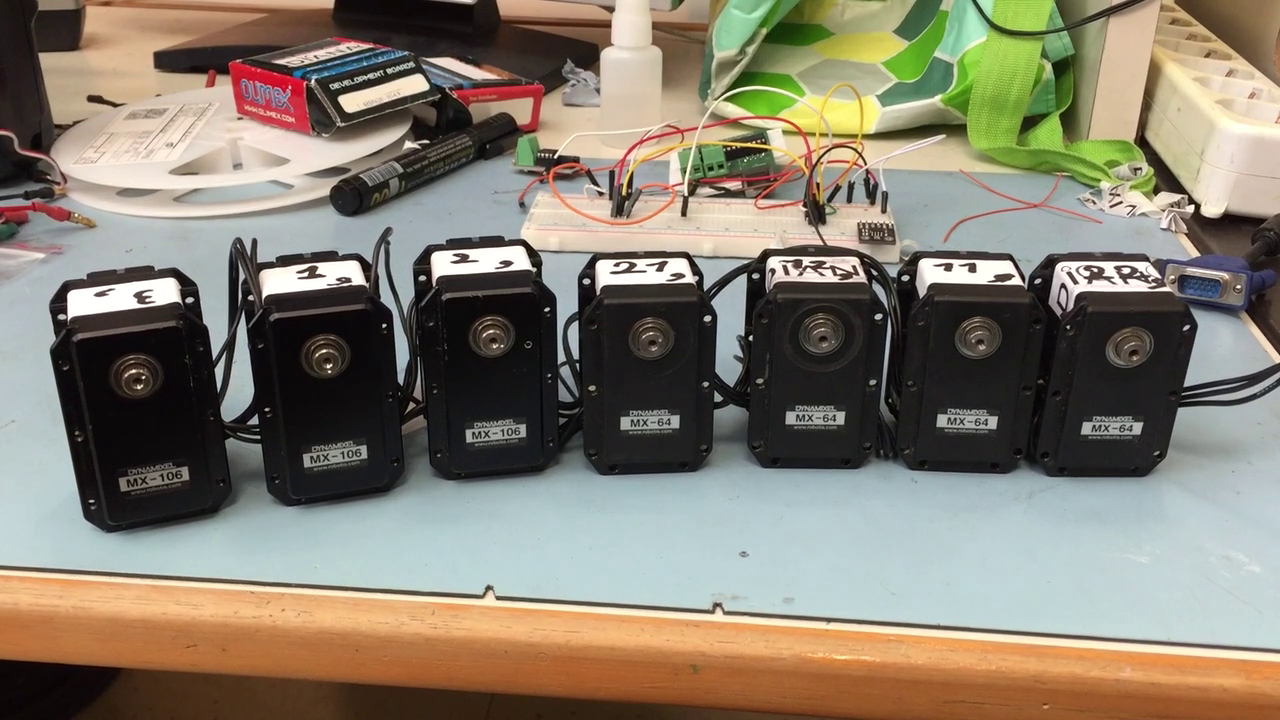
\includegraphics[width=0.6\textwidth]{image/dynamixel.png}
		\caption{Attuatori Dynamixel presenti a bordo del rover TRINITY durante un test di integrazione, a sinistra gli MX-106}
		\label{fig:MX160}
	\end{figure}

	\begin{figure}
		\centering
		\begin{tabular}{ll}
			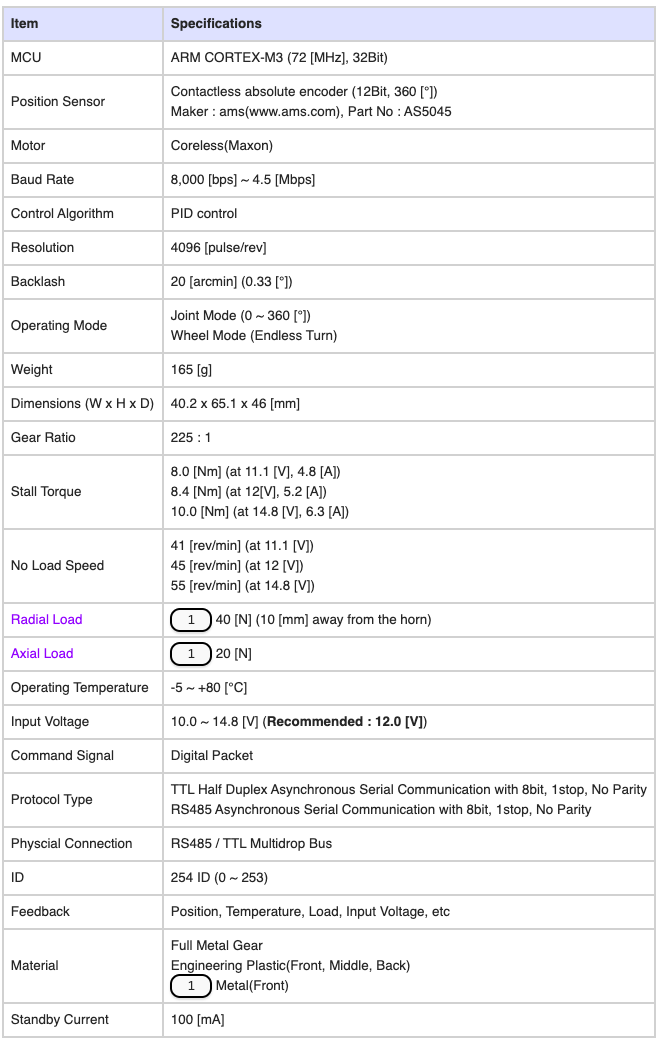
\includegraphics[width=0.4\textwidth]{image/mx160data.png}
			&
			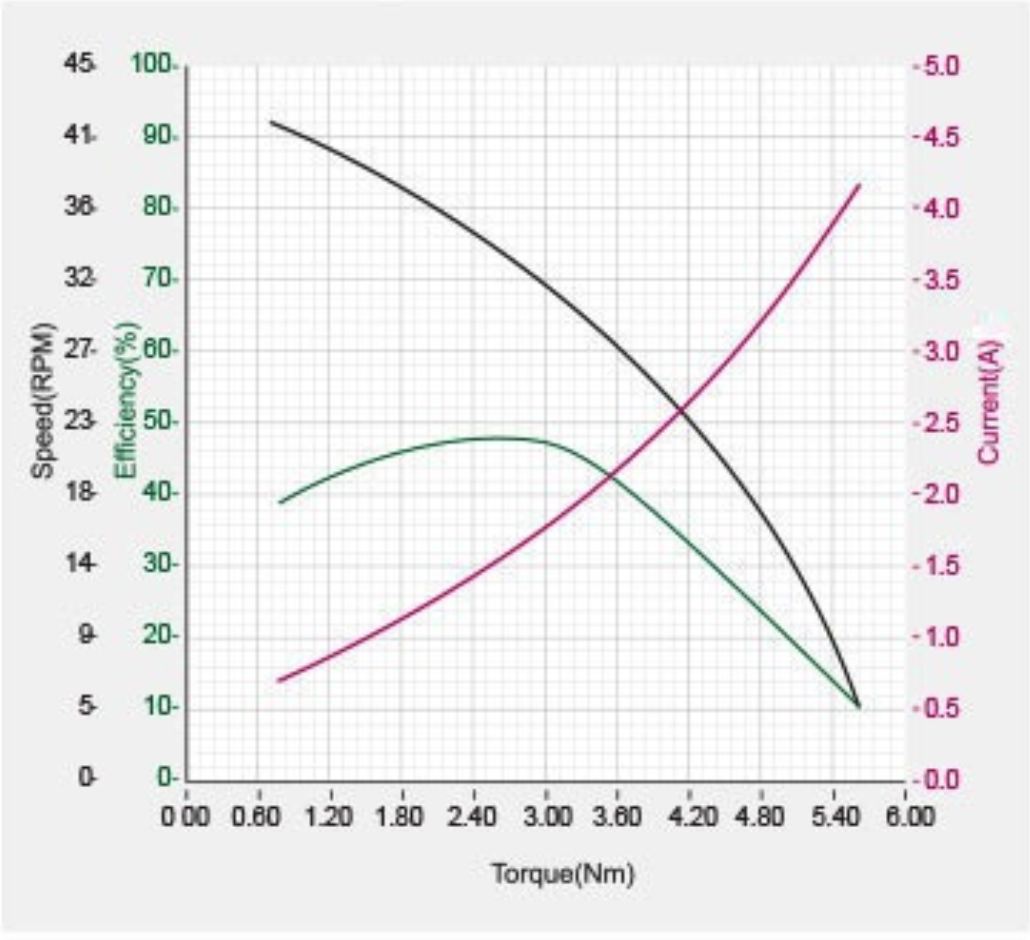
\includegraphics[width=0.4\textwidth]{image/mx160figure.png}
		\end{tabular}
		\caption{Caratteristiche tecniche dell'MX-106 FONTE Robotis E-Manual \cite{mx106}}
		\label{fig:MX160data}
	\end{figure}



	La ricerca è stata orientata quindi verso prodotti specifici per la robotica sperimentale. I servomotori \textit{ROBOTIS} sono emersi tra i più diffusi nel settore. Dal catalogo è stato selezionato il modello \textit{MX-106}. \\
	Dalla tabella delle caratteristiche fornite dal produttore in figura \ref{fig:MX160data} si evidenzia la compattezza, la leggerezza del componente e le possibilità di controllo offerte dal protocollo di comunicazione seriale implementabile sia su un microcontrollore sia su un computer dotato di interfaccia seriale.\\
	Guardando alla caratteristica meccanica in figura \ref{fig:MX160data} l'attuatore ha le performance migliori nell'intervallo di velocità tra 30 e 40 giri al minuto con una coppia massima di 3 Newton per metro. In questo intervallo si cercherà di progettare la trasmissione. \\
	
	Il produttore fornisce i modelli CAD tridimensionali del componente e delle flange di accoppiamento per l'albero di uscita scanalato. L'utilizzo di flange, dette \textit{horns}, permette di accoppiare all'albero di uscita scanalato componenti prodotti in manifattura additiva mediante viti. \\
	Ogni attuatore viene alimentato e riceve il bus dati attraverso un collegamento daisy chain, permettendo di realizzare una catena semplificando il cablaggio, che come vedremo per il polso sferico è delicato e soggetto a movimenti che ne causano la torsione. 

		
\chapter{Polso sferico, design e scelte progettuali}
	\section{Descrizione}
	\begin{figure}
		\centering
		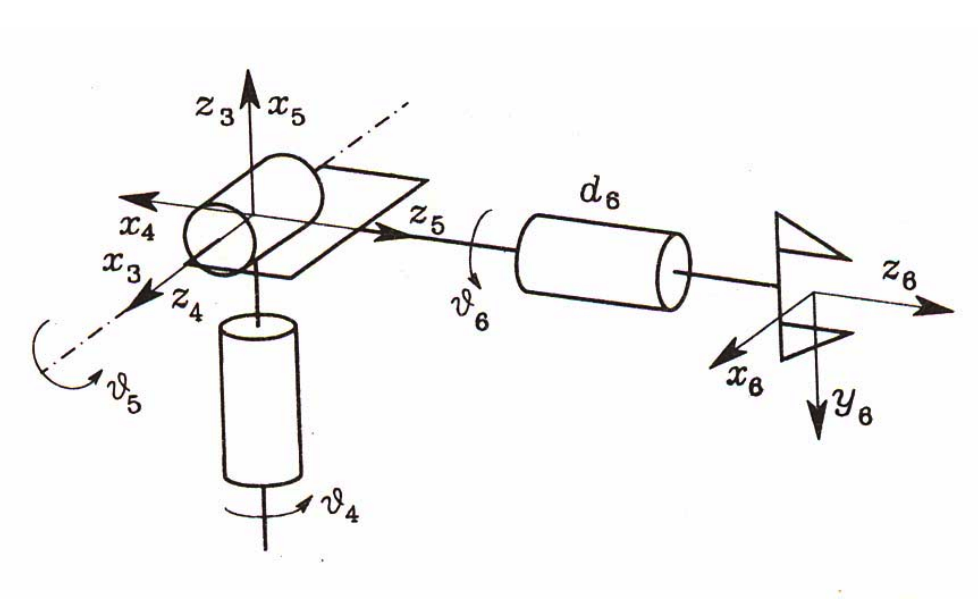
\includegraphics[width=0.6\textwidth]{image/sferico.png}
		\caption{Schema dei giunti del polso sferico con rappresentata una terna dell'utensile}
		\label{fig:sferico}
	\end{figure}
	Il polso sferico progettato per il manipolatore robotico del Rover TRINITY è un componente compatto, integrato e realizzato in manifattura additiva. 
	\begin{figure}
		\centering
		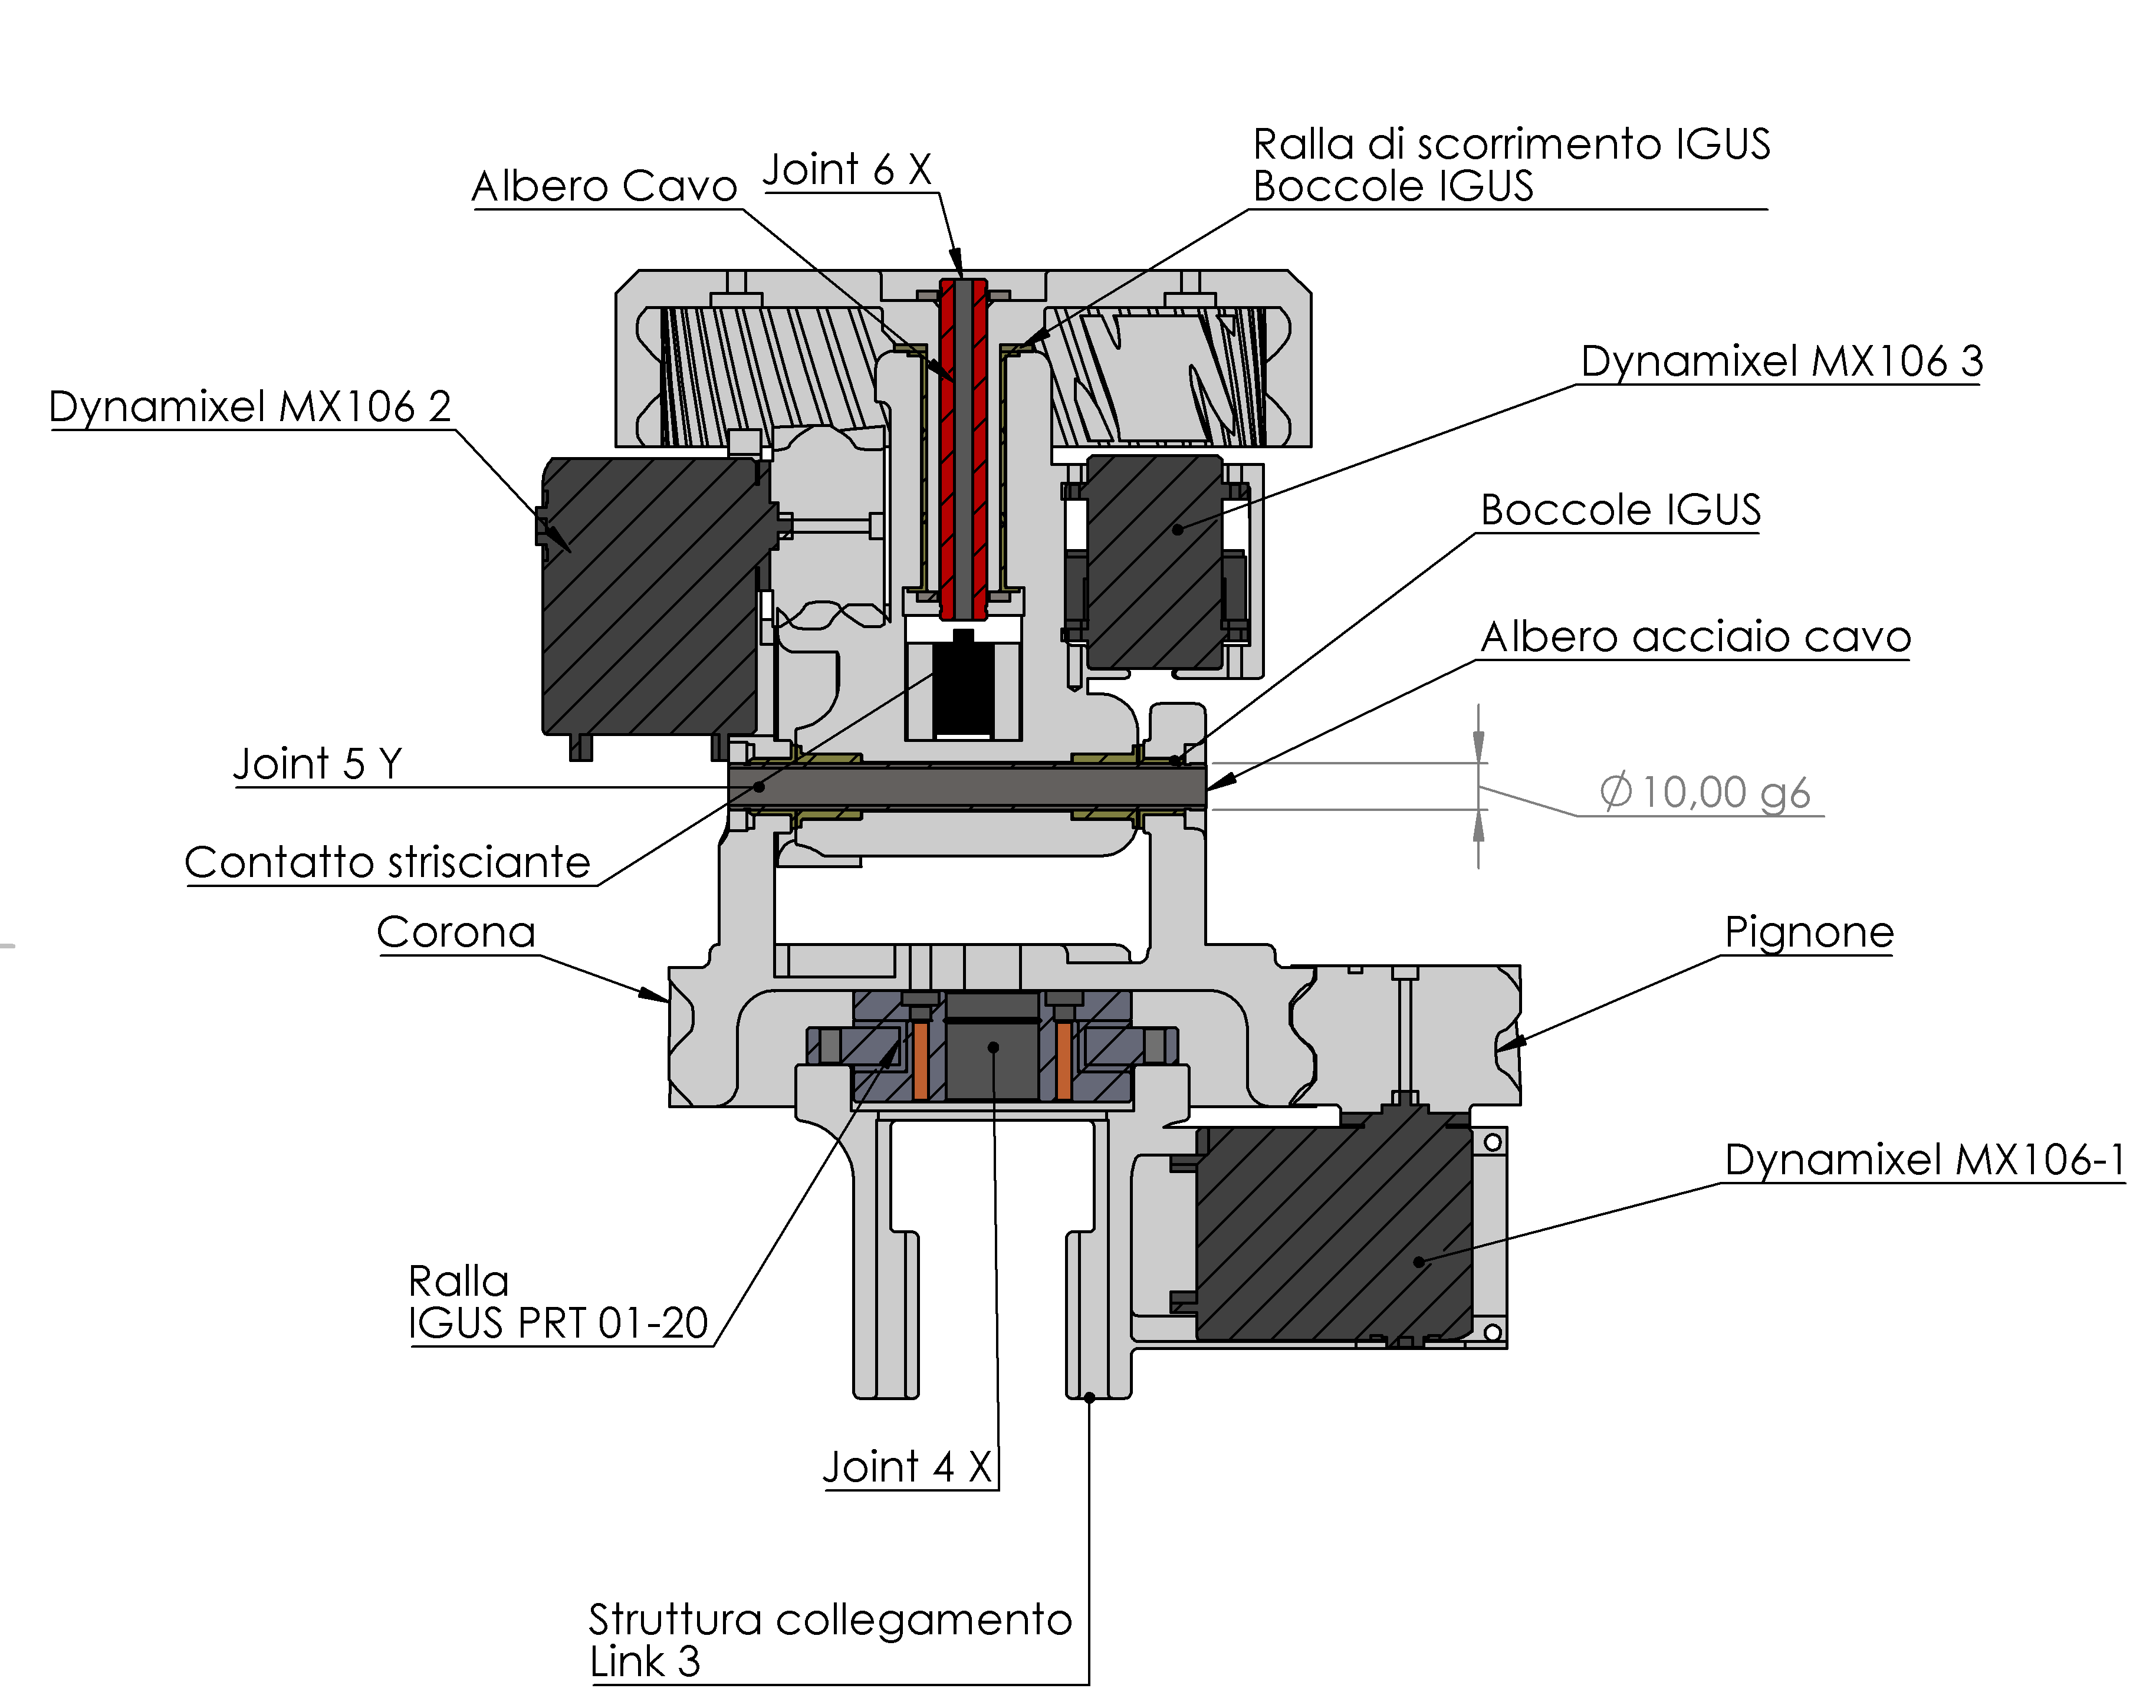
\includegraphics[width=1.2\textwidth]{Screen/wristsection.png}
		\caption{Sezione del componente realizzato con evidenziati i punti salienti trattati in questo capitolo}
		\label{fig:disegnosferico}
	\end{figure} 
	La caratteristica chiave di un polso sferico è il disaccoppiamento tra posizione e orientamento dell'utensile: il braccio ha il compito di posizionare il punto di origine della terna utensile, mentre il polso ne determina l'orientamento.\\
	La caratteristica che rende sferico il polso è l'intersezione dei tre assi di rotazione in un unico punto.
	
	
	\section{Studio del materiale da stampa ABSPlus P430}
	In funzione della possibilità di realizzare componenti in manifattura additiva presso i laboratori  del Dipartimento di Ingegneria Meccanica e Aerospaziale il Team DIANA ha deciso di approfondire la conoscenza delle risorse di produzione a disposizione. \\
	Il processo di stampa a deposizione di filamento (FDM) produce componenti caratterizzati da una struttura interna non isotropa, caratterizzata dalla presenza di layers e aree vuote.\\ 
	Nel caso della FDM il materiale non è isotropo. Nello specifico l’anisotropia è data sia dalla direzione della stampa (cioè la direzione dei piani depositati), dove è più resistente nella direzione parallela allo strato che in quella normale allo strato, sia dalla geometria dell’infill (geometrie che sostituiscono il volume interno pieno con un reticolato di aree vuote).\\
	 Pertanto è evidente che le proprietà meccaniche dipenderanno dalla direzione in cui sono applicati gli sforzi. 
	 Usando queste strutture si ottiene una struttura più leggera ma con proprietà non altrettanto inferiori. 
	 
	
	Il produttore del materiale e dell'attrezzatura di stampa fornisce una caratterizzazione del materiale isotropo, estruso come componente solido.\\
	 Questa condizione è però lontana dall'utilizzo reale, in quanto genera componenti estremamente costosi in termini di peso, tempo di lavorazione e quantità di materiale impiegato. \\
	Date le risorse a disposizione, al fine di realizzare un studio quantomeno indicativo sulle proprietà del materiale, è stato prodotto un set di provini e sottoposti a prova di trazione.\\
	Per le prove di trazione si segue la normativa \textit{ASTM D638 Standard method for Tensile Plastics}. Questa normativa permette di ottenere le proprietà a trazione di materiali polimerici sia semplici che rinforzati usando provini a forma di osso di cane. \\
	Il test è utilizzabile per campioni con spessore fino a 14 mm. Questo metodo inoltre permette di ottenere il modulo di poisson a temperatura ambiente. 
% Table generated by Excel2LaTeX from sheet 'Foglio1'
\begin{table}[htbp]
	\centering
	\caption{Dati sperimentali raccolti dalle prove effettuate}
	\begin{tabular}{|p{3.5em}|c|c|c|c|c|c|c|c|}
		\hline
		Item & \multicolumn{1}{p{3.5em}|}{Peso(g)} & \multicolumn{1}{p{3.5em}|}{Spessore (mm)} & \multicolumn{1}{p{3.5em}|}{Largh. (mm)} & \multicolumn{1}{p{3.5em}|}{area} & \multicolumn{1}{p{3.5em}|}{E (GPa)} & \multicolumn{1}{p{3.5em}|}{E (MPa)} & \multicolumn{1}{p{3.5em}|}{Tensile strength (MPa)} & \multicolumn{1}{p{3.5em}|}{Elong. (\%)} \bigstrut\\
		\hline
		\multicolumn{1}{|c|}{1} & 7,85  & 3,35  & 12,74 & 42,68 & 0,81  & 806,67 & 15,04 & 5,12 \bigstrut\\
		\hline
		\multicolumn{1}{|c|}{2} & 7,80  & 3,40  & 12,78 & 43,45 & 0,88  & 880,80 & 17,96 & 5,50 \bigstrut\\
		\hline
		\multicolumn{1}{|c|}{C}    & 7,83  & 3,39  & 12,80 & 43,38 & 0,96  & 955,62 & 16,54 & 5,21 \bigstrut\\
		\hline
		\multicolumn{1}{|c|}{3} & 8,71  & 3,45  & 12,95 & 44,68 & 0,91  & 907,36 & 16,46 & 5,09 \bigstrut\\
		\hline
		\multicolumn{1}{|c|}{4} & 8,75  & 3,40  & 12,87 & 43,76 & 0,89  & 885,46 & 15,76 & 4,88 \bigstrut\\
		\hline
		\multicolumn{1}{|c|}{M}     & 8,69  & 3,41  & 12,85 & 43,81 & 1,08  & 1083,89 & 19,26 & 5,37 \bigstrut\\
		\hline
		\multicolumn{1}{|c|}{5} & 9,86  & 3,48  & 12,80 & 44,54 & 1,18  & 1180,36 & 19,97 & 6,22 \bigstrut\\
		\hline
		\multicolumn{1}{|c|}{6} & 9,91  & 3,40  & 12,81 & 43,55 & 1,37  & 1371,50 & 22,02 & 7,22 \bigstrut\\
		\hline
		\multicolumn{1}{|c|}{P}     & 9,87  & 3,50  & 12,77 & 44,70 & 1,28  & 1280,19 & 21,91 & 7,01 \bigstrut\\
		\hline
	\end{tabular}%
	\label{tab:testdata}%
\end{table}%
	\begin{figure}
	\centering
	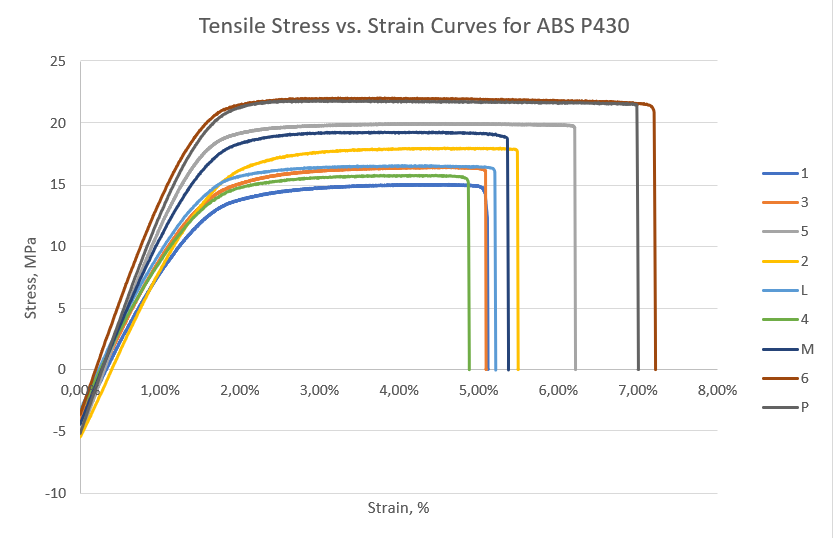
\includegraphics[width=0.7\textwidth]{Screen/curvesmaterial.png}
	\caption{Grafico Sforzo-Deformazione ottenuto }
	\label{fig:graficomateriale}
\end{figure} 

Si può concludere che ci sia una significativa differenza sia nel modulo elastico che nella tensile strength nei campioni con differente riempimento. \\
Con un minimo di 806,67 MPa, cioè il 58,81(\%) del valore massimo di 1371,508 MPa per il modulo elastico e un minimo di 15,04 MPa, cioè il 68,3(\%) del massimo di 22,02 MPa per la tensile strength si vede non solo una forte influenza del filling ma anche la mancanza di ripetibilità del meccanismo produttivo. \\
I campioni così stampati hanno valori circa della metà del materiale (Tensile strength = 44.81 Mpa, Modulo = 2.21 GPa) ma risultano superiori ai risultati trovati in letteratura \cite{P430paper}, questo risultato è da imputare probabilmente alla migliore adesione tra gli strati.

	\section{Integrazione e requisiti progettuali}
	I requirements che sono emersi dal primo studio di design sono :
	\begin{itemize}
		\item Tutta la parte in movimento del componente dovrà trovarsi all'interno dell'inviluppo sferico generato dalla rotazione del Joint 4 al fine di garantire che non ci siano zone interdette al moto.
		
		\item Sono neccessari dei passaggi per i cavi degli attuatori, quindi sono stati scelti alberi forati assialmente per le cerniere e predisposto un contatto strisciante a 12 conduttori per il Joint 6. I cavi passando all'interno degli alberi non rischiano di incastrarsi nei denti delle ruote dentate. 
		\item Minimo peso possibile per gli accessori, i cuscinetti sono un target su cui ridurre le masse.
		\item Da una prima considerazione delle potenze in gioco, confrontate col modello multbody e con la caratteristica meccanica dell'attuatore, è necessaria una riduzione con rapporto di almeno 2 per rendere possibile il funzionamento a pieno carico, tuttavia un rapporto 3 sarebbe ideale. 
		\item La precisione della stampante UPRINT verificata con delle prove di stampa di dentature non è sufficiente per realizzare un ingranamento di buona qualità al di sotto del modulo 2. 
		\item La stessa considerazione sulla precisione vale per i cuscinetti, che risultano avere sedi poco accurate. 
		
	\end{itemize}
	
	
	\section{Scelta dei Cuscinetti}
	I test effettuati sulla realizzazione di sedi per cuscinetti con la stampante UPRINT hanno dimostrato alcune criticità, peraltro diffuse e confermate dalla comunità di utilizzatori di stampa FDM per componenti meccanici. \\
	Le tolleranze dimensionali e di circolarità normalmente richieste per accoppiare un cuscinetto a corpi volventi sono state determinate per le lavorazioni tradizionali ad asportazione di truciolo. \`E semplice verificare la circolarità di una sede utilizzando un tornio o una rettificatrice, molto meno su un componente stampato in 3D. \\
	Il reparto meccanico del Team DIANA ha rilevato che le sedi realizzate non hanno una circolarità regolare e il diametro varia con le stampe in maniera non ripetibile. Pertanto un accoppiamento bloccato con forzamento (possibile con una piccola forza applicabile manualmente) risulta più sicuro di un accoppiamento incerto classico per cuscinetti. \\
	I cuscinetti a strisciamento IGUS sono dimensionati per il piantaggio in sede. Il dimensionamento definitivo si ottiene dopo adeguato piantaggio, pertanto le quote e le tolleranze vanno rilevate a boccola montata.
	Dopo alcune prove su piccoli componenti di prova è stata trovata una regola di tolleranza che garantiva un buon fissaggio sui diametri solitamente utilizzati dal reparto meccanico. \\
	Un altro vantaggio di questi cuscinetti è il peso irrisorio rispetto a un cuscinetto ad corpi volventi confrontabile, infatti la boccola $\phi$ 10 e lunghezza 10 pesa appena 3 grammi mentre il modello \textit{SKF 6200} ne pesa 30. 
	
	
	
	\section{Riduzione del numero minimo di denti: ingranamento elicoidale}\label{denti}
	Affinchè l'ingranamento tra due ruote dentate, come si apprende dal testo di Meccanica applicata alle meccaniche \cite{Jacazioteo} nel capitolo sulle trasmissioni mediante ruote dentate, avvenga in modo corretto è necessario che si abbia contatto delle superfici lungo il profilo ad evolvente dei denti. \\
	Il caso limite da evitare è quello in cui avviene una compenetrazione dei denti delle ruote, ossia interferenza. Per evitare l'interferenza è necessario che l'addendum, pari al modulo in un sistema modulare, assuma un valore tale da far cadere il punto di contatto all'interno del segmento di contatto. \\
	
	\begin{equation}\label{relazionedenti}
	\frac{a}{m}\leq\frac{z1}{2}\sqrt{\frac{1}{\tau^2}+(1+\frac{2}{\tau})\sin^2\alpha} -\frac{1}{\tau}
	\end{equation}
	Nella relazione \ref{relazionedenti} viene esplicitata la relazione che deve esserci tra addendum e il rapporto di trasmissione $\tau=\frac{r1}{r2}$ 
	
	\begin{equation}\label{relazionedenti2}
	Zmin=\frac{2[1+\sqrt{1+(2\tau+\tau^2)\sin^2\alpha}]}{(2+\tau)\sin^2\alpha}
	\end{equation}
	\\Se esplicitiamo il valore del numero di denti del pignone $Z_{min}$ otteniamo la relazione \ref{relazionedenti2}.
	Calcolando la formula per una rotismo con $\tau=\frac{1}{3}$ e angolo $\alpha=20$ otteniamo un valore $Zmin=17$.\\
	Questa condizione pone un limite progettuale piuttosto invasivo per la riduzione delle dimensioni. A parità di modulo si otterranno ruote di diametro maggiore se si vuole mantenere lo stesso rapporto di trasmissione. \\
	Produrre ingranaggi è un operazione tradizionalmente costosa e complessa a livello tecnologico: è richiesta una dentatrice oppure appositi utensili di forma già solo per ottenere una semplice dentatura a denti dritti. \\
	Produrre una dentatura elicoidale è ancora più complesso poichè richiede una variazione dell'angolo di incidenza della dentatrice e pertanto risulta sconveniente per realizzare un prototipo, dovendo ricorrere a ditte specializzate con costi elevati. \\
	La manifattura additiva rende disponibile un illimitato numero di forme e design, con la possibilità di integrare il componente strutturale con quello di trasmissione e realizzare pezzi unici dalle geometrie arbitrarie. \\
	Questa possibilità offerta dalla manifattura additiva apre sicuramente la strada alla valutazione di una dentatura elicoidale. \\
	Per calcolare il numero minimo di denti da assegnare ad una ruota elicoidale si fa riferimento ad una ruota fittizia a denti dritti per cui andremo a calcolare il numero minimo di denti.\\
	Bisogna ricordare infatti, come illustrato nel testo \cite{Jacazioteo} nel capitolo sulle ruote dentate elicoidali, che una ruota dentata elicoidale mantiene in ogni sezione effettuata da un piano frontale normale all'asse della ruota la forma di una evolvente del cilindro fondamentale. Tale proprietà non vale per una sezione normale all'elica primitiva e l'intersezione è rappresentata da un'ellisse con semiassi pari a $a=\frac{r}{cos\beta}$ e $b=r$ dove $\beta$ rappresenta l'angolo d'elica. 
	Pertanto è lecito considerare il moto relativo tra le due ruote come un moto di rotolamento tra i due cilindri avente asse inclinato di $\beta$ .
	
	\begin{equation}\label{dentivirtuale1}
	Z"=\frac{2R}{mn}=\frac{Z}{cos^3\beta}
	\end{equation}  
	
	Si considera che effettivamente l'ingranamento realizzato è quello di due ruote dentate a denti dritti aventi raggio $R=\frac{r}{\cos^2\beta}$, angolo di pressione $\alpha$ e numero di denti pari a $Z"$ come determinato nella relazione \ref{dentivirtuale1}
	
	\begin{equation}\label{dentivirtuale2}
	Z=Z" cos^3\beta
	\end{equation} 
	E ricavando il numero di denti reale $Z$ come in \ref{dentivirtuale2} otteniamo per la trasmissione studiata con angolo d'elica $\beta=20$ un valore di 14 denti. \\
	Con questo accorgimento si riesce a ridurre il numero minimo di denti del pignone ottenendo una riduzione dei diametri a parità di rapporto di trasmissione.\\
	 Si ottengono inoltre altri vantaggi noti dalla letteratura tecnica sulla costruzione e progetto di macchine :
	\begin{itemize}
		\item La variazione della distribuzione del carico sui denti avviene in maniera graduale 
		\item Gli urti sono ridotti essendoci più denti in presa contemporaneamente
		\item Il gioco tra i denti è di conseguenza ridotto, quindi si riduce il gioco angolare dell'ingranamento
	\end{itemize}

	\section{Dimensionamento della trasmissione}
	
	\subsection{Metodo di Lewis}
	Per un primo dimensionamento della trasmissione si è scelto di utilizzare il metodo di Lewis. \\
	Il dimensionamento di un ingranaggio, essendo nota la cinematica (rapporto di trasmissione, numeri di denti, angolo di pressione 
	 e angolo d’elica ), si effettua con la determinazione del modulo normale mn e della larghezza di fascia (sviluppo del dente nella
	direzione dell’asse di rotazione).\\
	 Nel caso di studio in oggetto la larghezza di fascia è molto condizionata dagli ingombri che devono avere i componenti e si è deciso di fissarla e determinare il modulo normale. \\
	Nel caso di dimensionamento statico vengono confrontate delle tensioni calcolate, rispettivamente una tensione di flessione (ottenuta tramite la formula di Lewis) e una dovuta al contatto hertziano (calcolata secondo le formule finali della teoria di Hertz), con una tensione ammissibile nel materiale ottenuta dividendo il carico di rottura (o snervamento) per un opportuno coefficiente di sicurezza. \\
	Nel caso del dimensionamento statico le tensioni massime calcolate sono ottenute considerando le forze massime scambiate dall’ingranaggio, quelle cioè che possono produrre rottura nel dente.\\
	Come carico massimo si è scelto di prendere a riferimento il valore di coppia di stallo, o holding torque, degli attuatori \textit{Dynamixel MX-106} pari a 8,4 Newton per metro. Difatti l'attuatore, in grado di misurare la corrente assorbita dal motore, correla il valore di soglia massima di corrente con la caratteristica elettrica del motore e disattiva l'alimentazione una volta raggiunta la coppia di stallo. \\
	Il calcolo statico a flessione di una ruota a denti elicoidali può eseguirsi estendendo opportunamente le formule valevoli per le ruote a denti dritti.
	\begin{equation}\label{torque}
	C=\frac{Ft}{\cos\beta}
	\end{equation}
	La forza che sollecita il dente, basata sull'ipotesi di singolo dente in presa valida per Lewis è \ref{torque}
	\begin{equation}\label{larghezza}
	b"=\frac{b}{\cos\beta}
	\end{equation}	
	La larghezza di fascia effettiva proiettata sul cilindro di contatto \ref{larghezza}
	\begin{equation}\label{sigmal}
	\sigma=\frac{\frac{Ft}{\cos\beta}}{\frac{b}{\cos\beta}m_{n}Y_{lw}}=\frac{Ft}{b m_{n}Y_{lw}}
	\end{equation}
	Quindi la tensione flessionale è ricavata in \ref{sigmal} considerando il coefficiente $Y_{lw}$ che si trova tabellato in letteratura tecnica
		\begin{equation}\label{mnlewis}
	mn=\sqrt[3]{\frac{Y_{lw} \cdot C \cdot 2 \cos\beta}{\frac{\sigma_{Yield}}{CS} \cdot b \cdot Z}}
	\end{equation}
	Esplicitando il modulo normale rispetto alla larghezza di fascia, alla coppia di sollecitazione e alla tensione di snervamento, considerato un opportuno coefficiente di sicurezza restituisce il modulo normale come in \ref{mnlewis}.
	\subsection{Contatto Hertziano}
	Il calcolo a contatto hertziano verifica che le pressioni specifiche di contatto, cioè le tensioni di tipo hertziano che si instaurano localmente durante l’ingranamento, siano inferiori alla tensione ammissibile del materiale, già definita per il calcolo statico a flessione.\\
	Un’eccessiva pressione specifica di contatto, infatti, comporterebbe un deterioramento della superficie del dente, inaccettabile ai fini di un corretto funzionamento dell’ingranaggio.\\
	Dal punto di vista del contatto hertziano due denti diritti che ingranano possono essere considerati come due cilindri a contatto lungo una generatrice di lunghezza pari alla larghezza di fascia del dente b. \\
	Il carico normale all’orma di contatto P è ancora la forza F che si scambiano i denti lungo la retta dei contatti. 
	\begin{equation}\label{hertz}
	\sigma_{H}=0,629\cdot0,418\cdot\sqrt{\frac{\frac{Ft}{\cos\alpha}\cdot E\cdot(\frac{1}{R_{1}}+\frac{1}{R_{2}})\cdot \frac{1}{\sin\alpha}}{\frac{b}{\cos\beta}}}\leq \frac{\sigma_{Yield}}{CS}
	\end{equation}
	
	La relazione con cui si effettua la verifica delle ruote elicoidali è \ref{hertz}
	
	\subsection{Codice di calcolo}
	\label{matlabcode}
	\begin{lstlisting}[language=Matlab]
	% La funzione lewis_factor ricerca all'iterno della tabella lewisdata
	% il valore opportuno per il coefficiente Y
	function [Y] = lewis_factor(Zn)
	load lewisdata
	i=1;
	while lewisdata.Z(i)<Zn
		i=i+1;
	end
	Y=lewisdata.Y(i);
	end
	
	%carico tabella dati di progetto 
	load data
	%coefficiente di sicurezza
	CS=2.5;
	CSHertz=1.2;
	
	%calcolo formula di Lewis, modulo normale
	data.mn=(lewis_factor(data.Z1)*(data.Cn*1000)*
	2*cosd(data.beta)/(data.sigmaS/CS)/
	data.larghezza/data.Z1)^(1/3);
	
	%calcolo rapporto di trasmissione
	data.tau=data.Z2/data.Z1;
	
	%calcolo raggi primitivi 
	R1=0.5*data.mn*data.Z1;
	R2=0.5*data.mn*data.Z2;
	
	%calcolo forze
	data.Ft=data.Cn*1000/R1;
	data.F0=data.Ft/cosd(data.alfa);
	data.Fr=data.F0*sind(data.alfa);
	F=data.Ft/cosd(data.alfa)/cosd(data.beta);
	data.Fa=F*sind(data.beta);
	
	%calcolo tensione di contatto Hertz
	data.sigmaH=0.629*0.418*((data.Ft/cosd(data.alfa))*
	(data.E*1000)*((1/R1)+(1/R2))*(1/sind(data.alfa))/
	(data.larghezza/cosd(data.beta)))^(1/2);
	
	if data.sigmaH<(data.sigmaS/CSHertz)
		data.Hertz="SI";
	else
		data.Hertz="NO";
	end
	%scrivo tabella risultati su file excel
	writetable(data,'POLSO.xls');
	\end{lstlisting}
	
		Per semplificare il processo di calcolo è stato utilizzato un semplice script in codice Matlab \ref{matlabcode} che calcola le grandezze necessarie al dimensionamento e il modulo normale a partire da una tabella \verb|data| contenente il numero di denti delle due ruote, la larghezza di fascia, gli angoli di pressione e di elica e le proprietà meccaniche del materiale. Sono inoltre calcolate le forze scambiate dai denti nei piani tangenziale, radiale, assiale.
		
		
		
		\subsection{Risultati Joint 4}
		
		Il Joint 4 rappresenta il primo grado di libertà del polso ed orienta la struttura lungo l'asse parallelo all'avambraccio. 
		Il risultato del calcolo di dimensionamento, tramite le considerazioni precedentemente fatte, ha prodotto un componente  che integra la ruota condotta con dimensioni compatibili ad ospitare il supporto per l'attuatore del joint 5 e la relativa cerniera.
			% Table generated by Excel2LaTeX from sheet 'Sheet1'
		\begin{table}[H]
			\centering
			\caption{Dati calcolati Joint 4}
			\begin{tabular}{rrrl}
				\multicolumn{1}{l}{\textbf{Z1}} & \multicolumn{1}{l}{\textbf{Z2}} & \multicolumn{1}{l}{\textbf{angolo pressione}} & \textbf{angolo elica} \\
				19    & 54    & 20°    & \multicolumn{1}{r}{20°} \\
				\multicolumn{1}{l}{\textbf{Ft [N]}} & \multicolumn{1}{l}{\textbf{F0 [N]}} & \multicolumn{1}{l}{\textbf{Fr [N]}} & \textbf{Fa [N]} \\
				383,8 & 408,8 & 139,7 & \multicolumn{1}{r}{148,638} \\
				\multicolumn{1}{l}{\textbf{modulo normale}} & \multicolumn{1}{l}{\textbf{Larghezza [mm]}} & \multicolumn{1}{l}{\textbf{Pressione contatto}} & \textbf{Verifica Hertz} \\
				2,304 & 30    & 11,3  & SI \\
			\end{tabular}%
			\label{tab:lewis1}%
		\end{table}%
	
	
		\begin{figure} [H]
			\centering
			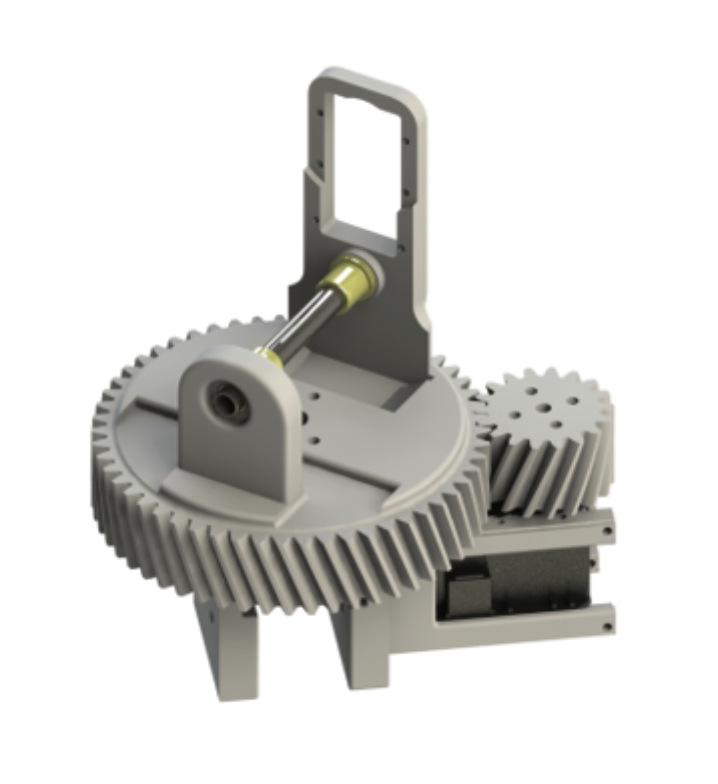
\includegraphics[width=0.6\textwidth]{Plots/POLSO1/wrist1.png}
			\caption{Ingranamento studiato per il Joint 4}
			\label{fig:wrist1}
		\end{figure} 
		Nella tabella \ref{tab:lewis1} troviamo i dati calcolati e in figura \ref{fig:wrist1} il modello CAD del componente integrato. 
	
		\begin{figure} [H]
			\centering
			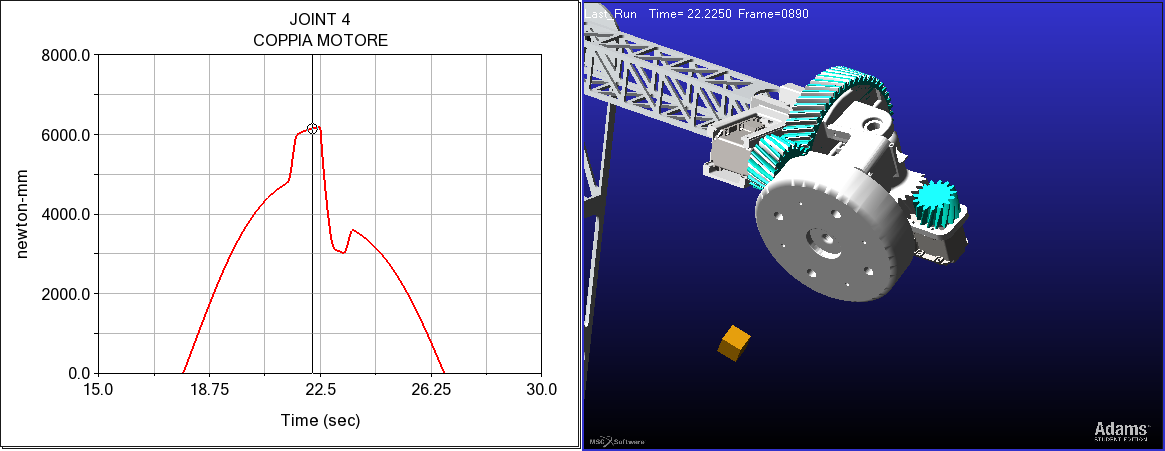
\includegraphics[width=1\textwidth]{Plots/POLSO1/polso1torque.png}
			\caption{Misura della coppia richiesta all'attuatore durante una rotazione in configurazione sfavolrevole per il Joint 4}
			\label{fig:MBDpolso1t}
		\end{figure} 
		\begin{figure} [H]
			\centering
			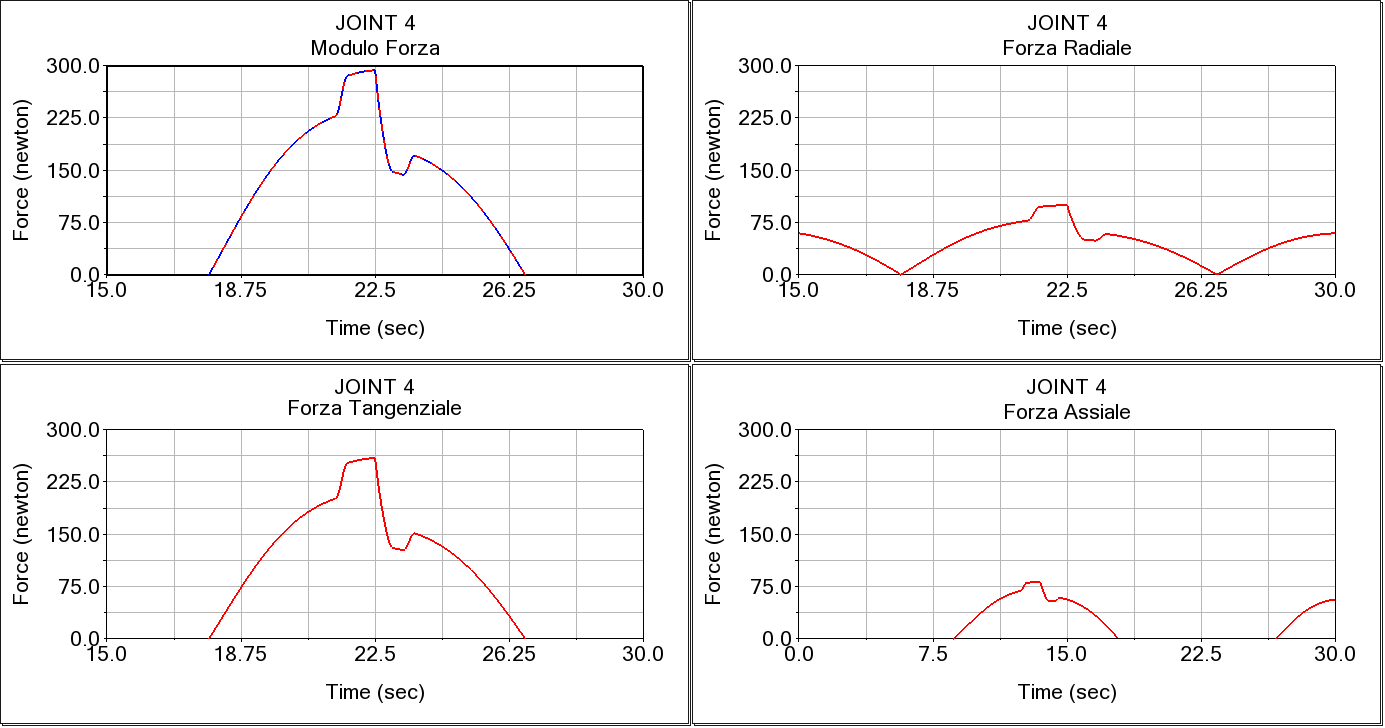
\includegraphics[width=1\textwidth]{Plots/POLSO1/polso1forces.png}
			\caption{Misura della forze scambiate nella trasmissione per il Joint 4}
			\label{fig:MBDpolso1f}
		\end{figure} 
		\begin{figure} [H]
			\centering
			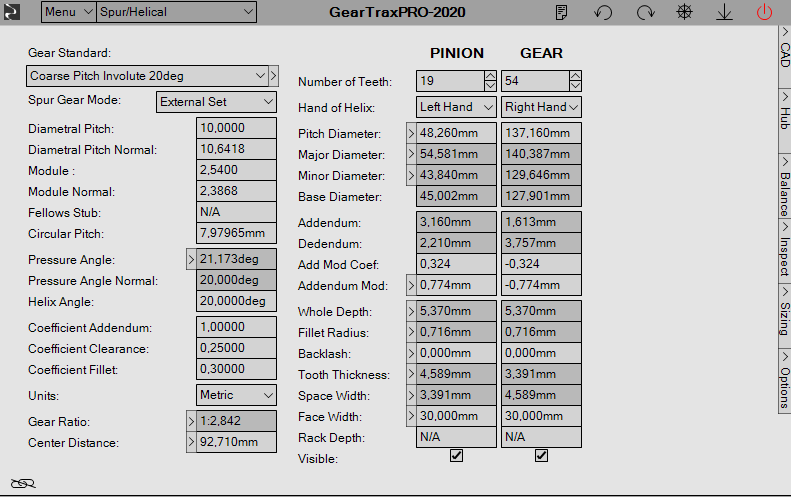
\includegraphics[width=0.5\textwidth]{Plots/POLSO1/gear_polso1.png}
			\caption{Parametri impostati nello script di design automatizzato GearTrax per il Joint 4}
			\label{fig:Gearpolso1}
		\end{figure} 
		Nel modello multibody è stata verificata la coppia richiesta all'attuatore durante una rotazione in configurazione sfavorevole in figura \ref{fig:MBDpolso1t} che risulta inferiore a quella massima di 8.4 Nm. Come verifica sono state misurate le forze di ingranamento in figura \ref{fig:MBDpolso1f} che sono confrontabili con quelle risultate dal calcolo analitico, considerando che il carico applicato è inferiore. Infine si è passati a generare l'accoppiamento di ruote dentate tramite il CAD con i parametri in figura \ref{fig:Gearpolso1}. Una volta generate le ruote dentate nell'ambiente \textit{Solidworks} è possibile modellarle come un qualsiasi altro componente e aggiungere le strutture necessarie, fori e sedi per cuscinetti.  
		
		\subsection{Risultati Joint 5}
		Il Joint 5 è perpendicolare al Joint 4 e contiene l'attuatore del Joint 6. Si tratta del giunto più problematico per una questione di ingombri ed è costituito da un componente di geometria complessa che integra :
		\begin{itemize}
			\item Il contatto strisciante per il passaggio della potenza all'end effector
			\item La ruota dentata condotta
			\item I cuscinetti della cerniera del Joint 6 
			\item La sede per l'attuatore del Joint 6 
		\end{itemize}
			\begin{figure} [H]
		\centering
		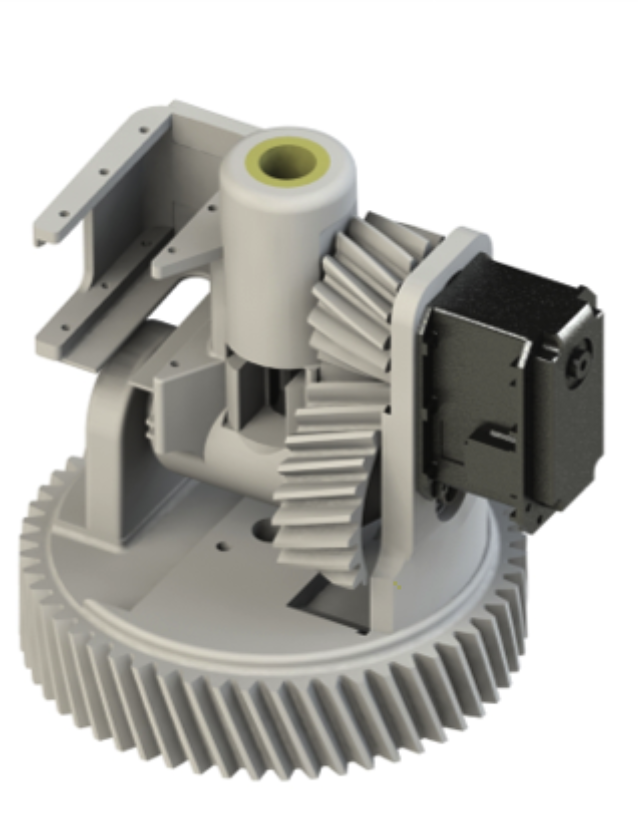
\includegraphics[width=0.4\textwidth]{Plots/POLSO2/wrist2.png}
		\caption{Ingranamento studiato per il Joint 5}
		\label{fig:wrist2}
	\end{figure} 
		\begin{table}[H]
			\centering
			\caption{Dati calcolati Joint 5}
			\begin{tabular}{rrrl}
				\multicolumn{1}{l}{\textbf{Z1}} & \multicolumn{1}{l}{\textbf{Z2}} & \multicolumn{1}{l}{\textbf{angolo pressione}} & \textbf{angolo elica} \\
				15    & 30    & 20°    & \multicolumn{1}{r}{20°} \\
				\multicolumn{1}{l}{\textbf{Ft [N]}} & \multicolumn{1}{l}{\textbf{F0 [N]}} & \multicolumn{1}{l}{\textbf{Fr [N]}} & \textbf{Fa [N]} \\
				405,5 & 431,5 & 147,5 & \multicolumn{1}{r}{157,05} \\
				\multicolumn{1}{l}{\textbf{modulo normale}} & \multicolumn{1}{l}{\textbf{Larghezza [mm]}} & \multicolumn{1}{l}{\textbf{Pressione contatto}} & \textbf{Verifica Hertz} \\
				2,56 & 24    & 14,06  & SI \\
			\end{tabular}%
			\label{tab:lewis2}%
		\end{table}%
	
		Pertanto per una questione di ingombri si è dovuto sacrificare il rapporto di trasmissione ed accontentarsi di una riduzione di rapporto 1 a 2. L'aumento di interasse avrebbe causato un allungamento del componente con relativo aumento di momento all'incastro del supporto che non superava la verifica statica svolta dal gruppo analisi FEM. 
		In questo caso la riduzione del numero minimo di denti trattata nel paragrafo \ref{denti} è stata fondamentale. 
		
		
	

		\begin{figure} [H]
			\centering
			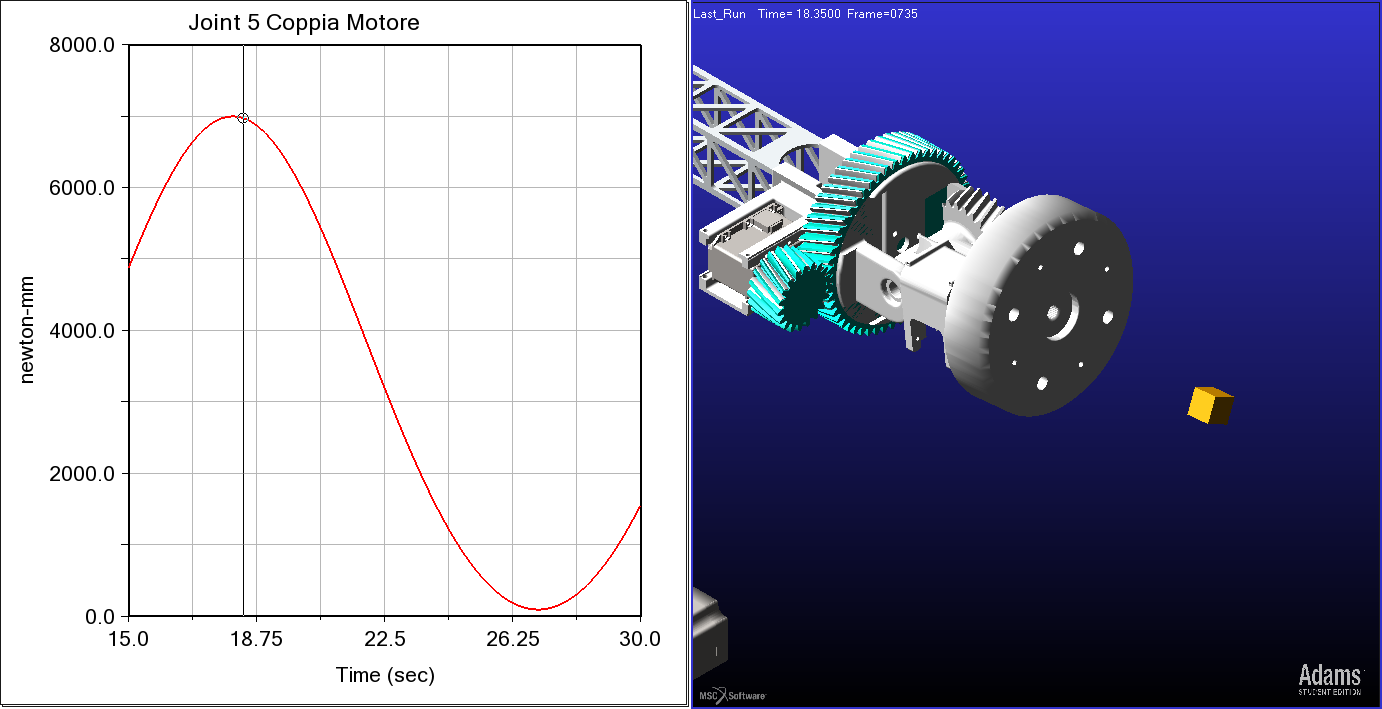
\includegraphics[width=1\textwidth]{Plots/POLSO2/polso2torque.png}
			\caption{Misura della coppia richiesta all'attuatore durante una rotazione in configurazione sfavolrevole per il Joint 5}
			\label{fig:MBDpolso2t}
		\end{figure} 
		\begin{figure} [H]
			\centering
			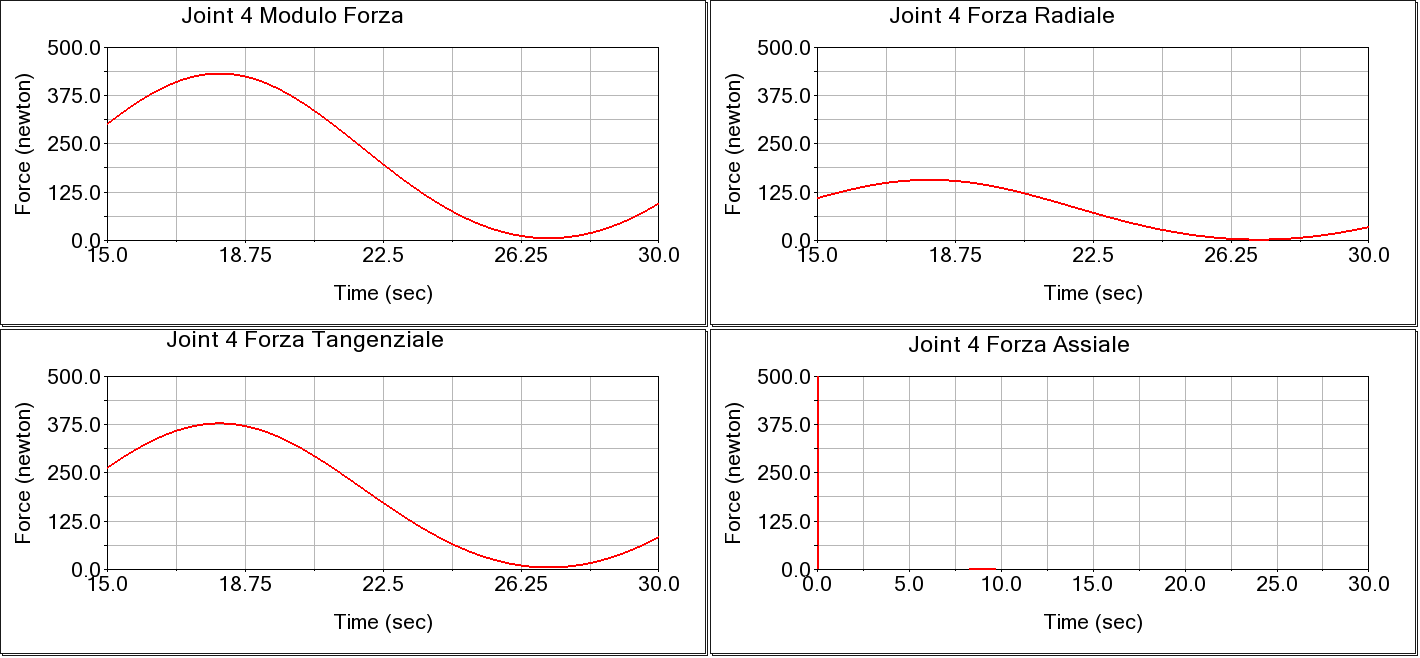
\includegraphics[width=1\textwidth]{Plots/POLSO2/polso2forces.png}
			\caption{Misura della forze scambiate nella trasmissione per il Joint 5}
			\label{fig:MBDpolso2f}
		\end{figure} 
		\begin{figure} [H]
			\centering
			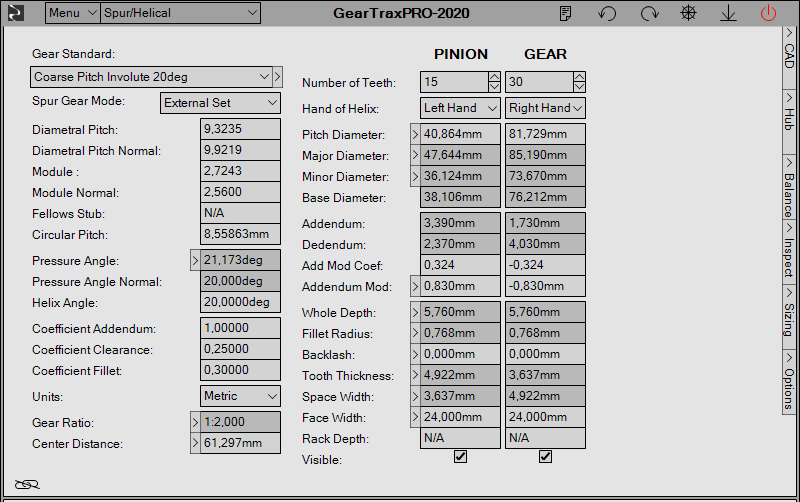
\includegraphics[width=0.6\textwidth]{Plots/POLSO2/gear_polso2.png}
			\caption{Parametri impostati nello script di design automatizzato GearTrax per il Joint 5}
			\label{fig:Gearpolso2}
		\end{figure} 
		I valori calcolati in tabella \ref{tab:lewis2} mostrano valori maggiori delle sollecitazioni rispetto al Joint 4 e richiedono un modulo più grande. 
		Il modello multibody ha permesso di verificare la coppia massima richiesta all'attuatore, che sfiora valori limite \ref{fig:MBDpolso2t} senza superarli e le forze di ingranamento \ref{fig:MBDpolso2f} confrontabili con quelle calcolate.
		L'ingranamento è stato poi modellato come in figura \ref{fig:Gearpolso2} per poi costruire il resto della geometria mediante la definizione di piani paralleli e perpendicolari a quello frontale della ruota dentata. 
		
	
	
	\subsection{Risultati Joint 6}
		Il Joint 6 provedde alla rotazione del tool sul suo asse ed è parallelo al Joint 4. 
	
		\begin{table}[H]
		\centering
		\caption{Dati calcolati Joint 6}
		\begin{tabular}{rrrl}
			\multicolumn{1}{l}{\textbf{Z1}} & \multicolumn{1}{l}{\textbf{Z2}} & \multicolumn{1}{l}{\textbf{angolo pressione}} & \textbf{angolo elica} \\
			19    & 54    & 20°    & \multicolumn{1}{r}{20°} \\
			\multicolumn{1}{l}{\textbf{Ft [N]}} & \multicolumn{1}{l}{\textbf{F0 [N]}} & \multicolumn{1}{l}{\textbf{Fr [N]}} & \textbf{Fa [N]} \\
			383,8 & 408,8 & 139,7 & \multicolumn{1}{r}{148,638} \\
			\multicolumn{1}{l}{\textbf{modulo normale}} & \multicolumn{1}{l}{\textbf{Larghezza [mm]}} & \multicolumn{1}{l}{\textbf{Pressione contatto}} & \textbf{Verifica Hertz} \\
			2,304 & 30    & 11,3  & SI \\
		\end{tabular}%
		\label{tab:lewis3}%
	\end{table}%


	\begin{figure} [H]
		\centering
		\includegraphics[width=0.6\textwidth]{Plots/POLSO3/gear_polso3.png}
		\caption{Parametri impostati nello script di design automatizzato GearTrax per il Joint 6}
		\label{fig:Gearpolso3}
	\end{figure} 
	Il Joint 6 fornisce la piastra di attacco con l'end effector ed è stato dimensionato in analogia al Joint 4 per semplificare il controllo. Esso differisce dal Joint 4 in quanto l'ingranamento è di due ruote interne ed è stato previsto nel firmware dell'attuatore l'inversione del senso di rotazione, così da essere sempre concorde col Joint 4. Strutturalmente e meccanicamente è il meno sollecitato della struttura e lo si considera verificato per analogia al Joint 4, si riportano in tabella \ref{tab:lewis3} e in figura \ref{fig:Gearpolso3} i valori scelti per la costruzione. 
	
		\subsection{Disegno di ruote dentate elicoidali prodotte in FDM}
		Per realizzare i modelli CAD delle ruote dentate calcolate, noto il modulo, il numero di denti, gli angoli caratteristici e la larghezza di fascia sono possibili diversi metodi.\\ 
		Quello che appare più accessibile di prima analisi consiste nell' utilizzare le capacità parametriche del \textit{ CAD Solidworks}, riportando la sezione di un dente ed estrudendolo lungo la generatrice dell'elica cilindrica. \\
		Questo approccio trova subito un limite pratico: correggere il design per la necessità di una modifica implica ricominciare dall'inizio la modellazione e poco si adatta a una progettazione iterativa. \\
		Un approccio iterativo è stato necessario vista la necessità di coniugare i risultati di calcolo di dimensionamento con gli ingombri delle ruote e il collocamento degli attuatori sul polso.\\
		 Soprattutto nel Joint 5 \ref{fig:wrist2} il collocamento dell'attuatore per movimentare il Joint 6 è piuttosto complesso e doveva rispettare gli spessori minimi per la sede dell'albero, le dimensioni del Dynamixel e l'interasse della ruota interna del Joint 6. \\
		Un software di disegno automatizzato di questi componenti è stato di grande aiuto nel realizzare velocemente i componenti e per poter fare variazioni e tentativi nel valutare la soluzione migliore. \\
		
		Il software \textit{GearTrax}, introdotto nel corso di Disegno di Macchine, prende il controllo del CAD e automaticamente genera le geometrie una volta configurati tutti i parametri che troviamo in figura \ref{fig:Gearpolso1} e \ref{fig:Gearpolso2} e \ref{fig:Gearpolso3}.
			
		
	

	%\section{Dimensionamento di un rotismo stampato in 3D, compromessi e assunzioni}
	%\section{Risultati ottenuti dal dimensionamento}
	

\chapter{Costruzione mediante manifattura additiva e assemblaggio}
Nella realizzazione di un prototipo la parte indubbiamente più interessante dopo la progettazione e la realizzazione dei modelli CAD è quella della costruzione del componente.\\
 La manifattura additiva, al contrario delle tecnologie tradizionali che spesso richiedono una dotazione di macchine da officina e materiali da lavorare disponibili presso un'azienda esterna, ha concesso spesso agli studenti del \textit{Team DIANA} di vedere realizzati rapidamente i propri progetti e di partecipare al processo di produzione.\\
  Una volta prodotti i componenti in FDM, programmati i servomotori e ricevuti i cuscinetti e la viteria necessaria è stato possibile assemblare il polso sferico. 
	\section{Produzione dei componenti}
		\begin{figure}
		\centering
		\begin{tabular}{lll}
		\includegraphics[width=0.35\textwidth]{Screen/pack1.png}
		&
		\includegraphics[width=0.35\textwidth]{Screen/pack2.png}
		&
		\includegraphics[width=0.35\textwidth]{Screen/pack3.png}
		\end{tabular}
		\caption{Pack di stampa in output dal software di slicing }
		\label{fig:pack}
		\end{figure} 
	\begin{figure}
		\centering
		\begin{tabular}{ll}
		\includegraphics[height=6cm,keepaspectratio]{image/uprint.jpg}
		&
		\includegraphics[height=6cm,keepaspectratio]{image/uprintp.jpg}
		\end{tabular}	
	\caption{Stampante Stratasys UPRINT SE e pack in fase di stampa}
	\label{fig:uprint}
	\end{figure}	
	La fase di produzione di un componente FDM parte dalla generazione del codice in linguaggio G-CODE per il controllo delle macchine utensili. 
	La generazione del codice viene svolta in maniera automatizzata da un software di slicing, in questo caso da parte di \textit{Stratasys CatalystEX},  proprietario della stampante, che contiene già tutti i parametri necessari per una corretta configurazione della stampa. \\
	All'utente spetta solo la collocazione dei manufatti da realizzare all'interno del \textit{pack}, una rappresentazione del volume di stampa che ha come base la tavoletta removibile su cui vengono depositati i materiali.\\
	 Un fattore importante è la scelta dell'orientazione spaziale dei componenti e nel caso delle ruote dentate è assolutamente mandatorio adagiarle su un piano frontale e facendo si che l'estrusione sviluppi il dente in altezza, in modo che ogni layer contenga una sezione del dente che conservi il profilo ad evolvente.\\ Come vediamo nella fotografia \ref{fig:uprint} i componenti dentati vengono estrusi sul piano frontale, assieme alle eventuali strutture di supporto in colore più chiaro che andranno rimosse. \\
	Sono stati prodotti 3 pack, per un tempo di stampa totale predetto dal software di 55 ore, in figura \ref{fig:pack}.\\
	Una volta terminata la fase di stampa si procede alla rimozione della tavoletta e si staccano i pezzi, ripulendoli dai supporti di colore più chiaro che servono a sostenere le geometrie che sono sospese o in aggetto. 
	Dopo la pulizia sono necessarie la sbavatura e la rifinitura mediante carta abrasiva sottile, limetta e taglierino al fine di rimuovere bave e filamenti interrotti. 
	
	\section{Analisi dei costi}
	In questa fase analizzeremo il costo di produzione di questo componente mediante manifattura FDM e il costo dei componenti accessori e degli attuatori. 
	Il costo di un componente prodotto con questa tecnica è spesso elevato, ma giustificato dall'economia di poter produrre un singolo prototipo senza particolari costi di attrezzaggio e ordine di quantità minime di materiale. 
	Il materiale utilizzato sia per la costruzione che per il supporto è fornito dalla produttrice della stampante in bobine da $700 cm^3$ per un costo al $cm^3$ di Euro 0,33. 
	\begin{table}[H]
		\centering
		\caption{Costi di Stampa 3D}
		\begin{tabular}{rr|r|r|r|}
			\hline
			\multicolumn{1}{|l|}{\textbf{Pack}} & \multicolumn{1}{l|}{\textbf{Volume materiale [$cm^{3}$]}} & \multicolumn{1}{l|}{\textbf{Volume supporto [$cm^{3}$]}} & \multicolumn{1}{l|}{\textbf{costo [€ ]}} & \multicolumn{1}{l|}{\textbf{ore stampa}} \bigstrut\\
			\hline
			\multicolumn{1}{|r|}{1} & 265,82 & 120,2 & 123,53 & 29,5 \bigstrut\\
			\hline
			\multicolumn{1}{|r|}{2} & 155,56 & 58,13 & 68,38 & 16 \bigstrut\\
			\hline
			\multicolumn{1}{|r|}{3} & 143,22 & 13,25 & 50,07 & 9 \bigstrut\\
			\hline
			&       & \textbf{TOTALE} & 241,98 & 54,5 \bigstrut\\
			\cline{3-5}    \end{tabular}%
		\label{tab:printcost}%
	\end{table}%
	In tabella \ref{tab:printcost} riportiamo i costi di stampa dei 3 pack realizzati, riferiti alle quantità di materiale predette dal software \textit{CatalystEX}. Il costo è sicuramente elevato, essendo il materiale originale usato dalla stampante, che tuttavia ha garantito un risultato positivo al primo tentativo senza sprechi di materiale. 
	
	% Table generated by Excel2LaTeX from sheet 'Foglio1'
	\begin{table}[H]
		\centering
		\caption{Costi di realizzazione}
		\begin{tabular}{rrr|r|r|}
			\hline
			\multicolumn{1}{|l|}{\textbf{Numero}} & \multicolumn{2}{c|}{\textbf{Articolo}} & \multicolumn{1}{l|}{\textbf{costo [€]}} & \multicolumn{1}{l|}{\textbf{Totale [€]}} \bigstrut\\
			\hline
			\multicolumn{1}{|r|}{3} & \multicolumn{2}{c|}{Dynamixel MX-106} & 450   & 1350 \bigstrut\\
			\hline
			\multicolumn{1}{|r|}{1} & \multicolumn{2}{c|}{IGUS PRT-01-20} & 43    & 43 \bigstrut\\
			\hline
			\multicolumn{1}{|r|}{4} & \multicolumn{2}{c|}{IGUS JFM 1014} & 2,95  & 11,8 \bigstrut\\
			\hline
			\multicolumn{1}{|r|}{2} & \multicolumn{2}{c|}{IGUS JFM 1618} & 3,1   & 6,2 \bigstrut\\
			\hline
			\multicolumn{1}{|r|}{1} & \multicolumn{2}{c|}{IGUS JSM 1618} & 2,8   & 2,8 \bigstrut\\
			\hline
			\multicolumn{1}{|r|}{2} & \multicolumn{2}{c|}{Albero MISUMi FPSPJFF} & 13    & 26 \bigstrut\\
			\hline
			\multicolumn{1}{|r|}{} & \multicolumn{2}{c|}{STAMPA 3D} &       & 241,98 \bigstrut\\
			\hline
			&       &       & \textbf{TOTALE} & 1681,78 \bigstrut\\
			\cline{4-5}    \end{tabular}%
		\label{tab:projectcost}%
	\end{table}%
	Nella tabella \ref{tab:projectcost} invece riportiamo il costo totale di stampa sommato a tutti gli altri componenti necessari all'assemblaggio. Spicca sicuramente il costo dei 3 attuatori Dynamixel, che essendo componenti specialistici per robotica hanno sicuramente dei costi elevati, pur rappresentando un oggetto molto durevole nel tempo. Gli attuatori sono stati infatti riciclati da un precedente progetto del Team DIANA risalente al 2010. 
	\section{Assemblaggio}
	\begin{figure}
		\centering
		\begin{tabular}{lll}
			\includegraphics[width=0.33\textwidth]{image/w1.jpg}
			&
			\includegraphics[width=0.33\textwidth]{image/w2.jpg}
			&
			\includegraphics[width=0.33\textwidth]{image/w3.jpg}
		\end{tabular}
		\caption{Polso assemblato per la prima volta dopo la fase di produzione e corredato dei servomotori}
		\label{fig:wristassembled}
	\end{figure}
	L'assemblaggio del componente è molto semplice e facilmente intuibile dalla sezione \ref{fig:sferico}. Una volta collocata la ralla \textit{IGUS PRT 01 20} sul link 3 ed inserito in sede il primo attuatore completo di pignone è possibile avvitare alla ralla il link 4. Si inseriscono le boccole nelle rispettive sedi del link 4 e del link 5 e si avvitano i Dynamixel 2 e 3 in sede con viti M2. \'E possibile inserire il link 5 e l'albero della cerniera e una volta ruotato connettere i pignoni ai Dynamixel. Si completa l'assemblaggio con l'inserimento del link 6 completo di albero e si blocca con anelli seeger.\\
	I cablaggi passano all'interno degli alberi e sono completati di connettori saldati e ricoperti di guaina termorestringente e connessi al contatto strisciante per poter portare potenza e segnale all'end effector. \\
	Una volta completato il cablaggio e controllato con il multimetro l'assenza di cortocircuiti e la correttezza dei collegamenti è possibile alimentare gli attuatori con un alimentatore da banco a tensione di 12 Volt. \\
	
	\begin{figure}
		\centering
		\includegraphics[width=0.6\textwidth]{image/wizard.png}
		
		\caption{Software Dynamixel Wizard, permette di accedere a tutta la control table degli attuatori serie MX tramite un'interfaccia grafica}
		\label{fig:wizard}
	\end{figure}
	
	Tramite il software \textit{Dynamixel Wizard} ed un'interfaccia seriale USB è possibile connettere al PC gli attuatori ed effettuare la configurazione. \\
	Per configurare il polso è necessario :
	\begin{itemize}
		\item Assegnare il baud rate di 57600 bps corrispondente  al valore 34 dell'indirizzo 4 della Control Table
		\item Assegnare un ID corretto ad ogni attuatore all'indirizzo 3
		\item Inviare il comando di Torque Enable=1 all'indirizzo 24, questo farà andare in coppia gli attuatori
		\item Inviare Moving Speed = 300 all'indirizzo 32 corrispondente a 10 rpm 
		\item Inviare  Goal Position=0 all'indirizzo 30
		\item Verificare lo scostamento dallo zero e compensare con il comando Multi Turn Offset all'indirizzo 20 finchè non sarà tutto centrato
		
	\end{itemize}
	Una volta configurato è possibile sospendere l'alimentazione e i valori settati saranno conservati nella EEPROM degli attuatori oppure continuare ad inviare posizioni per verificare che vengano raggiunte. 
	Il raggiungimento di posizioni interdette causa un urto ed un bloccaggio, che viene risolto dal sistema di sicurezza di coppia massima degli attuatori che impedisce la rottura dei componenti o del servomotore. 
	
\chapter{Risultati attesi ed ottenuti dal Robot realizzato}
	\section{Test e collaudo del Robot assemblato}
	Una volta conclusa la produzione del polso sferico il robot è stato completamente assemblato e dopo aver completato anche il cablaggio e l'installazione dell'elettronica è iniziata una fase di collaudo e di familiarizzazione con i comandi. 
	\begin{figure}
		\centering
		\begin{tabular}{ll}
		\includegraphics[width=0.4\textwidth]{image/armfoto.jpg}
		&
		\includegraphics[width=0.4\textwidth]{image/baseass.jpg}
		\end{tabular}
		\caption{Braccio robotico in fase di assemblaggio e cablaggio}
		\label{fig:ass1}
	\end{figure}
\begin{figure}
	\centering
	\begin{tabular}{ll}
		\includegraphics[width=0.4\textwidth]{image/5kg1.png}
		&
		\includegraphics[width=0.4\textwidth]{image/5kg2.png}
	\end{tabular}
	\caption{Test di sollevamento di un carico da 5 chilogrammi}
	\label{fig:test1}
\end{figure}
\begin{figure}
	\centering
		\includegraphics[width=0.6\textwidth]{Screen/coppelia.png}
	\caption{Modello di simulazione robotica VREP, riceve lo stesso input dell'elettronica di controllo}
	\label{fig:coppelia}
\end{figure}
\begin{figure}
	\centering
	\begin{tabular}{ll}
		\includegraphics[height=8cm,keepaspectratio]{image/cace.png}
		&
		\includegraphics[height=8cm,keepaspectratio]{image/mant.jpg}
	\end{tabular}
	\caption{Test di raccolta cache e operazione di manutenzione}
	\label{fig:test2}
\end{figure}	
 	Essendo infatti il robot un prototipo completamente sperimentale, al di là del modello di simulazione è stato necessario testare a lungo il suo funzionamento e comprendere i comandi da impartire agli attuatori. 
 	Il modello della posizione attesa viene visualizzato a schermo nell'ambiente di simulazione robotica \textit{VREP} come in figura \ref{fig:coppelia}. Si confronta poi la posizione ottenuta in realtà dal robot col modello, misurando con metro e goniometro, e poi corregendo il software di controllo adattandolo se necessario. 
 	Dopo una serie di esperimenti si è ottenuto un robot molto preciso nei movimenti, caratteristica notata anche dalla giuria della competizione European Rover Challenge. 
 	I test sono proseguiti con il sollevamento un carico equivalente a quello imposto nelle simulazioni multibody di 5 chilogrammi come in figura \ref{fig:test1} e simulando in laboratorio alcune task come in foto \ref{fig:test2}. 
 	I risultati in sede di competizione si possono vedere anche nelle foto \ref{fig:maintanance} \ref{fig:cache} \ref{fig:science} \ref{fig:torocache} anticipate nel primo capitolo per descrivere le task operative della competizione. I risultati, per quanto riguarda il manipolatore sono stati buoni ed hanno permesso di raggiungere un notevole punteggio nelle task in cui le capacità di manipolazione erano centrali. 
 		


\backmatter
\chapter{Disegni ed elaborati tecnici}
\includepdf{draws/Arm.pdf}
\includepdf{draws/1.pdf}
\includepdf{draws/2.pdf}
\includepdf{draws/3.pdf}
\includepdf{draws/3b.pdf}
\includepdf{draws/45.pdf}
\includepdf{draws/56.pdf}


\begin{thebibliography}{9}
\bibitem{ERC2019} European Rover Challenge, \emph{Student Rules}, ERC, gennaio 2019

\bibitem{RobotSpong}Mark W. Spong, Seth Hutchinson, and M. Vidyasagar, \emph{Robot Modeling and Control}, JOHN WILEY  

\bibitem{RobotSiciliano}Bruno Siciliano • Lorenzo Sciavicco Luigi Villani • Giuseppe Oriolo \emph{Robotics: Modelling, Planning and Control}, SPRINGER

\bibitem{Jacazioes}Giovanni Jacazio, Stefano Pastorelli \emph{Esercizi di meccanica applicata alle macchine}, Levrotto e Bella

\bibitem{Jacazioteo}Giovanni Jacazio, Stefano Pastorelli \emph{Meccanica applicata alle macchine}, Levrotto e Bella

\bibitem{P430paper} R. Henandez, D. Slaughter, D. Whaley, J. Tate, B. Asiabanpour, Analyzing the tensile, compressive and flexural properties of 3D printed ABS P430 plastic based on printing orientation using fused deposition modeling, Proceedings of the 26th Annual International Solid Freeform Fabrication Symposium – An Additive Manufacturing Conference, 2016

\bibitem{mx106} MX-106T/R - ROBOTIS e-Manual \url{http://emanual.robotis.com/docs/en/dxl/mx/mx-106/}
\end{thebibliography}

\end{document}

% altri riferimenti da usare come esempi.

\bibitem{ERC2019} European Rover Challenge, \emph{Student Rules}, ERC, gennaio 2019
	
	
\bibitem{Robot}Giovanni Jacazio, Stefano Pastorelli \emph{Esercizi di meccanica applicata alle macchine}, Levrotto e Bella

\bibitem{bigliano2010} Bigliano M., \emph{Sicurezza nell'installazione di un velivolo 
		senza pilota MALE; applicazione di metodologia di Zonal Safety 
		Analysis al velivolo del Progetto SAvE}, Politecnico di Torino, 
		maggio 2010
\bibitem{astrid2012} Chiesa S., Di Meo G.A., Fioriti M., Medici G., Viola N.,
		\emph{ASTRID - Aircraft on board Systems sizing and TRade-off 
		analysis in Initial Design}, Research Bulletin, Warsaw University 
		of Technology, Institute of Aeronautics and Applied Mechanics, 
		p. 1-28, 17-19, ottobre 2012

